\documentclass{beamer}
\usetheme{Antibes} % Antibes Dresden Frankfurt
\setbeamertemplate{navigation symbols}{} 
\usefonttheme[onlymath]{serif}
\usecolortheme{default}
\setbeamertemplate{navigation symbols}{} 
\usepackage{amsmath}
\usepackage[T1]{fontenc}
\usepackage{lmodern}
\usepackage{mathrsfs}
\usefonttheme[onlymath]{serif}
\usepackage{siunitx}
\usepackage{tikz}
\usetikzlibrary{arrows}
\usepackage{perpage}
\MakePerPage{footnote}
% \usepackage{showframe} 

\setbeamerfont{page number in head/foot}{size=\footnotesize}
\setbeamertemplate{footline}[frame number]

\newcommand{\scs}{\scriptsize}

\usepackage{graphicx}
\graphicspath{{.}{images/}}


\title[Novel Optical Effects in Functionalized Graphene: 
Formalism and Simulations]
{Novel Optical Effects in Functionalized Graphene: 
Formalism and Simulations}
\author{Reinaldo Arturo Zapata Pe\~na}
\institute{Centro de Investigaciones en \'Optica, A.C.}
\date{December 8, 2017}


%%%%%%%%%%%%%%%%%%%%%%%%%%%%%%%%%%%%%%%%%%%%%%%%%%%%%%%%%%%%%%%%%%%%%%%%%%%%%
%%%%%%%%%%%%%%%%%%%%%%%%%%%%%%%%%%%%%%%%%%%%%%%%%%%%%%%%%%%%%%%%%%%%%%%%%%%%%
%%%%%%%%%%%%%%%%%%%%%%%%%%%%%%%%%%%%%%%%%%%%%%%%%%%%%%%%%%%%%%%%%%%%%%%%%%%%%

\begin{document}




%%%%%%%%%%%%%%%%%%%%%%%%%%%%%%%%%%%%%%%%%%%%%%%%%%%%%%%%%%%%%%%%%%%%%%%%%%%%%
\section*{The project}
%%%%%%%%%%%%%%%%%%%%%%%%%%%%%%%%%%%%%%%%%%%%%%%%%%%%%%%%%%%%%%%%%%%%%%%%%%%%%





\begin{frame}
\maketitle
\end{frame}




% %%%%%%%%%%%%%%%%%%%%%%%%%%%%%%%%%%%%%%%%%%%%%%%%%%%%%%%%%%%%%%%%%%%%%%%%%%%%%
% \section{Introduction}
% %%%%%%%%%%%%%%%%%%%%%%%%%%%%%%%%%%%%%%%%%%%%%%%%%%%%%%%%%%%%%%%%%%%%%%%%%%%%%



% %%%%%%%%%%%%%%%%%%%%%%%
% \subsection{Structure}
% %%%%%%%%%%%%%%%%%%%%%%%


% \begin{frame}
% \begin{center}
% 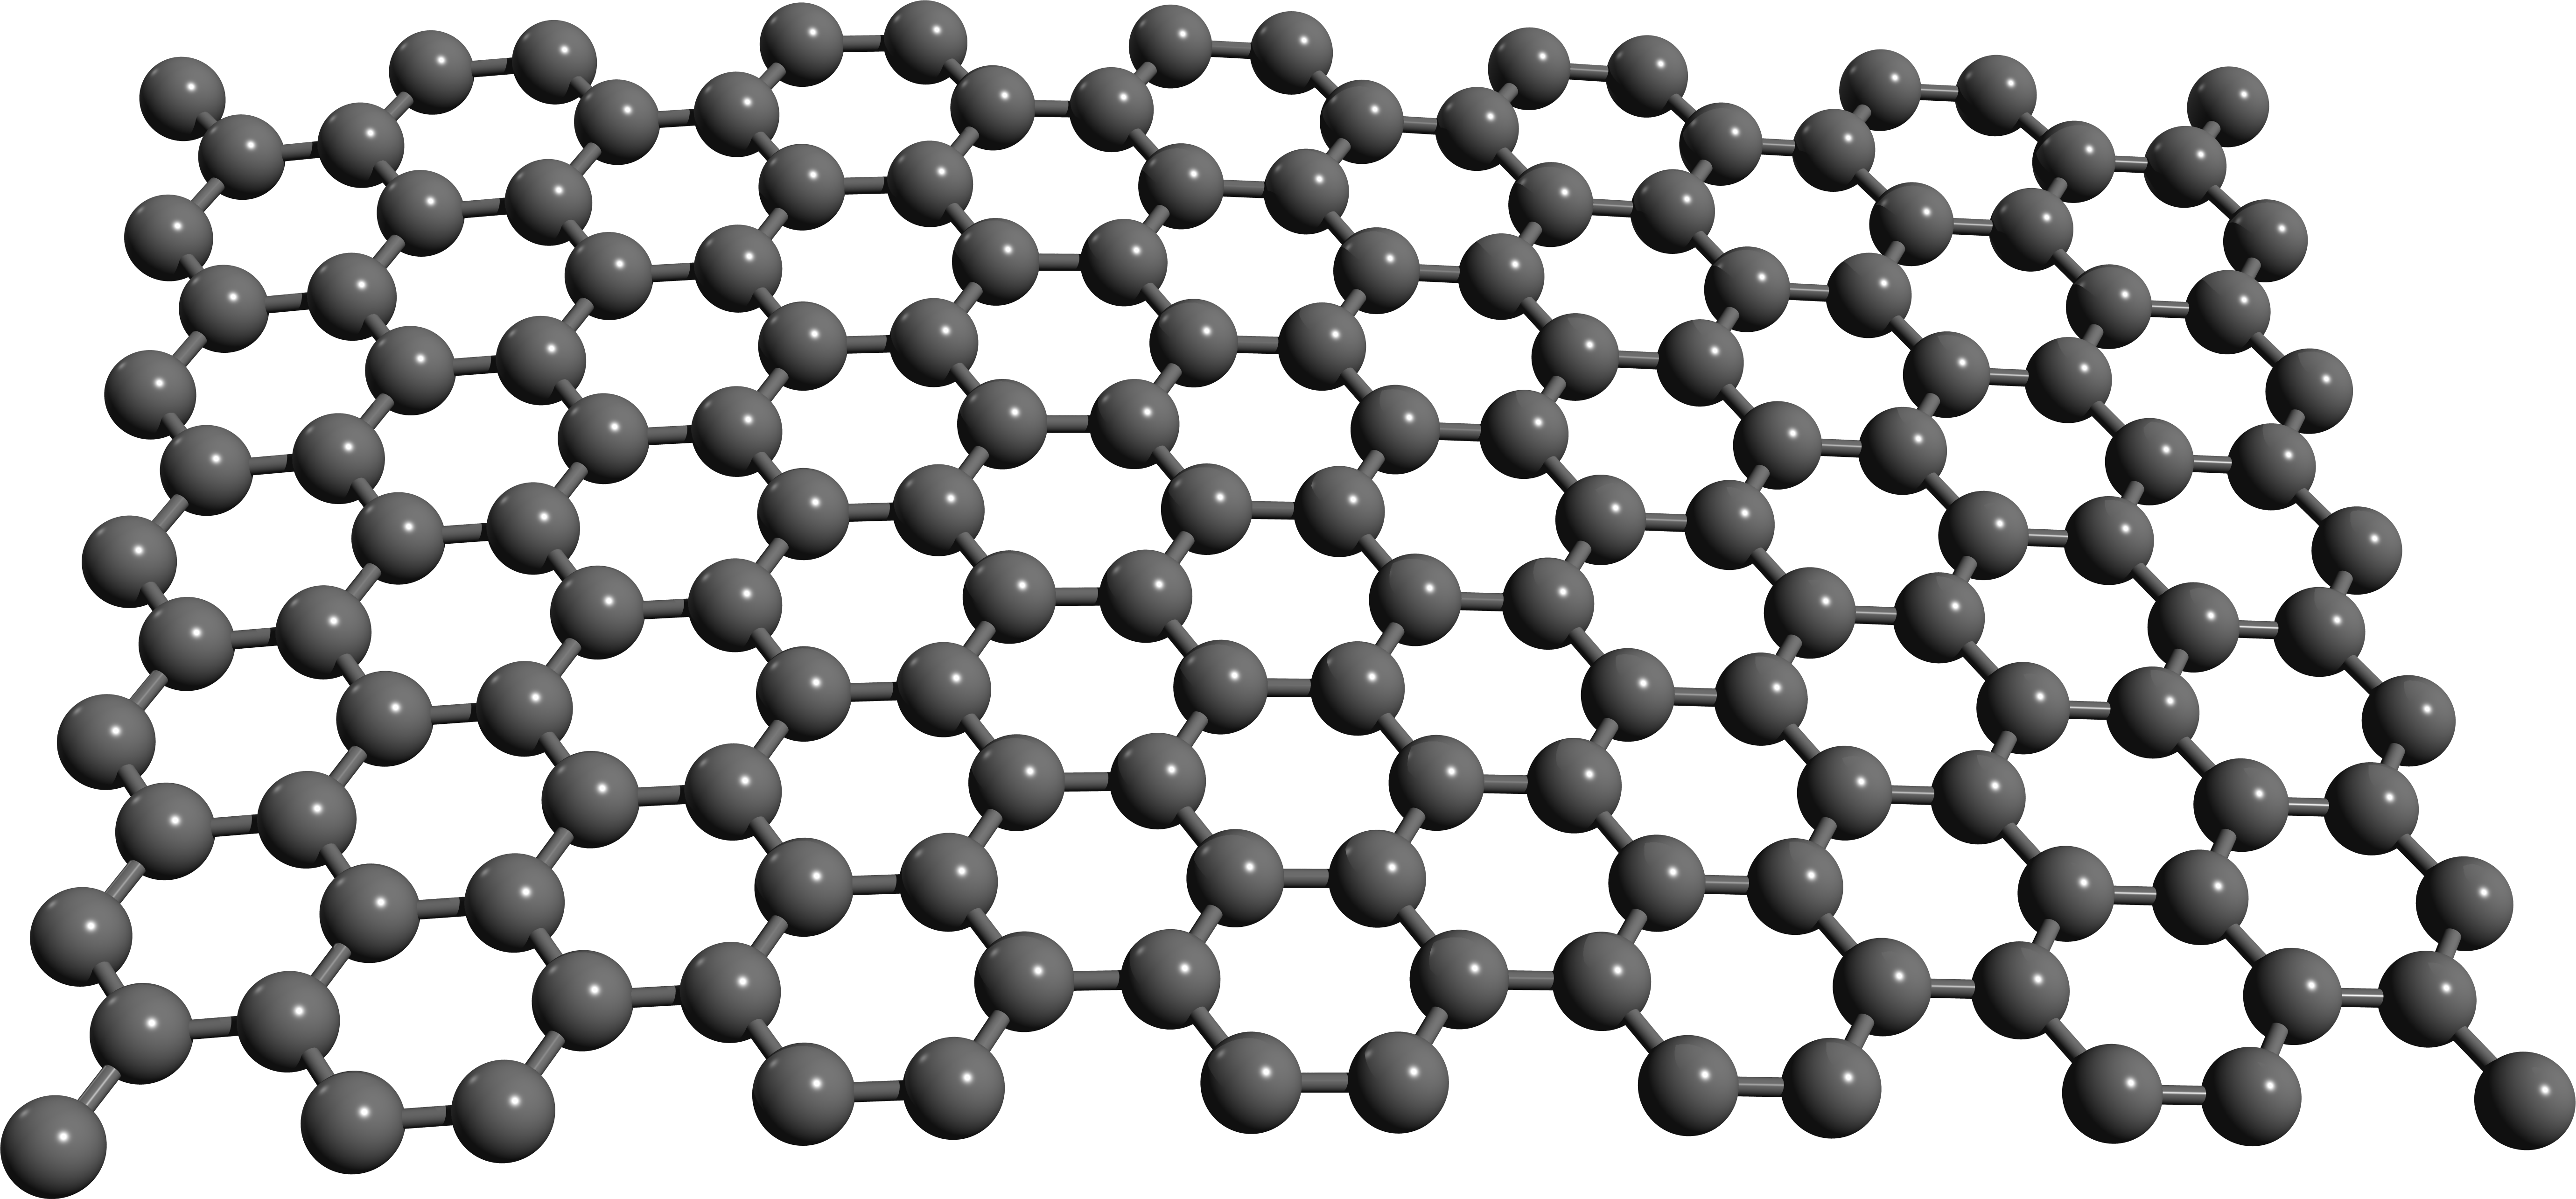
\includegraphics[width=0.9\textwidth]{figs/graphene2.png}
    
% {\Huge Graphene structure}

% Hexagonal lattice with carbon atoms in each vertex. 

% \end{center}
% \end{frame}


% %%%%%%%%%%%%%%%%%%%%%%%%%%%%%%%%%%%%%%%%%%%%%%%%%%%%%%%%%%%%%%%%%%%%%%%%%%%%%


% %%%%%%%%%%%%%%%%%%%%%%%
% \subsection{Properties}
% %%%%%%%%%%%%%%%%%%%%%%%

% \begin{frame}

% \vspace{-0.3cm}

% \noindent\makebox[\linewidth]{\rule{\linewidth}{0.4pt}}

% \vspace{-2.0mm}
% \begin{center}
% {\huge General properties of graphene}
% \end{center}

% \vspace{-6mm}
% \noindent\makebox[\linewidth]{\rule{\linewidth}{0.4pt}}

% \vfill

% \begin{columns}
% \column{0.6\textwidth}

% \begin{center}
% 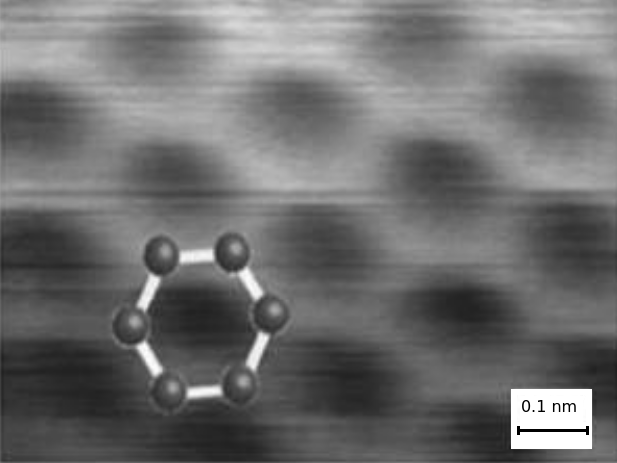
\includegraphics[width=0.8\textwidth]{figs/tem.png}

% Transmission electron microscopy of graphene.
% \footnote[frame]{\tiny E. Stolyarova, et al. PNAS, 104(22):9209, 2007.}
% \end{center}


% \column{0.5 \textwidth}
% \begin{itemize}

% \item Good heat conductor
% \footnote[frame]{\tiny A.K. Geim and K.S. Novoselov. Nature
% Materials, 6(3):183-191, 2007.}

% \item Extremely strong
% \footnote[frame]{\tiny C. Lee, et al. Science, 321(5887):385-388, 2008.}

% \item Flexible
% \footnote[frame]{\tiny Briggs, B. D. et. al. App. Phys. Lett. 97:
% 223102. 2010.}

% \end{itemize}
% \end{columns}

% \hspace{5mm}

% \end{frame}

% %%%%%%%%%%%%%%%%%%%%%%%%%%%%%%%%%%%%%%%%%%%%%%%%%%%%%%%%%%%%%%%%%%%%%%%%%%%%%

% \begin{frame}
% \vspace{-0.3cm}

% \noindent\makebox[\linewidth]{\rule{\linewidth}{0.4pt}}

% \vspace{-2.0mm}
% \begin{center}
% {\huge Electronic properties of graphene}
% \end{center}

% \vspace{-6mm}
% \noindent\makebox[\linewidth]{\rule{\linewidth}{0.4pt}}

% \vfill

% \begin{columns}
% \column{0.5\textwidth}
% \begin{itemize}

% \item Quantum Hall effect at room temperature
% \footnote[frame]{\tiny K.S. Novoselov, A.K. Geim, et al. Nature,
% 438(7065):197-200, 2005.}

% \item Excellent electrical current conduction
% \footnote[frame]{\tiny A.K. Geim and K.S. Novoselov. Nature
% Materials, 6(3):183-191, 2007.}

% % \item Dirac Cones\textsuperscript{ 2}

% \item Transparent to visible light
% \footnote[frame]{\tiny R.R. Nair, et al. Science, 320(5881):1308-1308, 2008.}

% \item Tunable bandgap
% \footnote[frame]{\tiny M.Y. Han, et. al. Physical Review Letters,
% 98(20):206805, 2007}



% \end{itemize}
% \column{0.5\textwidth}
% \begin{figure}
% \centering
% 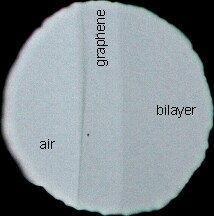
\includegraphics[width=0.65\textwidth]{figs/trasparency.jpg}

% Photograph of graphene \\
% in transmitted light.
% \footnote[frame]{\tiny By Rahul Nair - Manchester group.}
% \end{figure}
% \end{columns}

% \hspace{5mm}
% \end{frame}

% %%%%%%%%%%%%%%%%%%%%%%%%%%%%%%%%%%%%%%%%%%%%%%%%%%%%%%%%%%%%%%%%%%%%%%%%%%%%%

% \begin{frame}

% \begin{columns}

% \column{0.4\textwidth}

% \begin{itemize}
% \item Tunable bandgap by:
% \noindent
% \begin{itemize}

% \item[-] changing sheet size
% \footnote[frame]{\tiny C. Feng et al. 2009. Jour. of Chem. Phis. 131:194702,
% 2009. \label{ft:fengJCP09}}

% \item[-] changing number of sheets and stacking\textsuperscript{
% \ref{ft:fengJCP09}}

% \item[-] applying an electric field
% \footnote[frame]{\tiny Y. Zhang et al. Nature, 459(7248):820-823, 2009.
% \label{ft:ahangNAT09}}

% \item[-] doping
% \footnote[frame]{\tiny T. Ohta et al. Science, 313(5789):951-954, 2006.
% \label{ft:ohtaSC06}}

% \item[-] hydrogenation
% \footnote[frame]{\tiny D.C. Elias et al. Science, 323(5914):610-613, 2009.
% \label{ft:eliasSC09}}

% \end{itemize}
% \end{itemize}

% \column{0.7\textwidth}


% \begin{center}
% 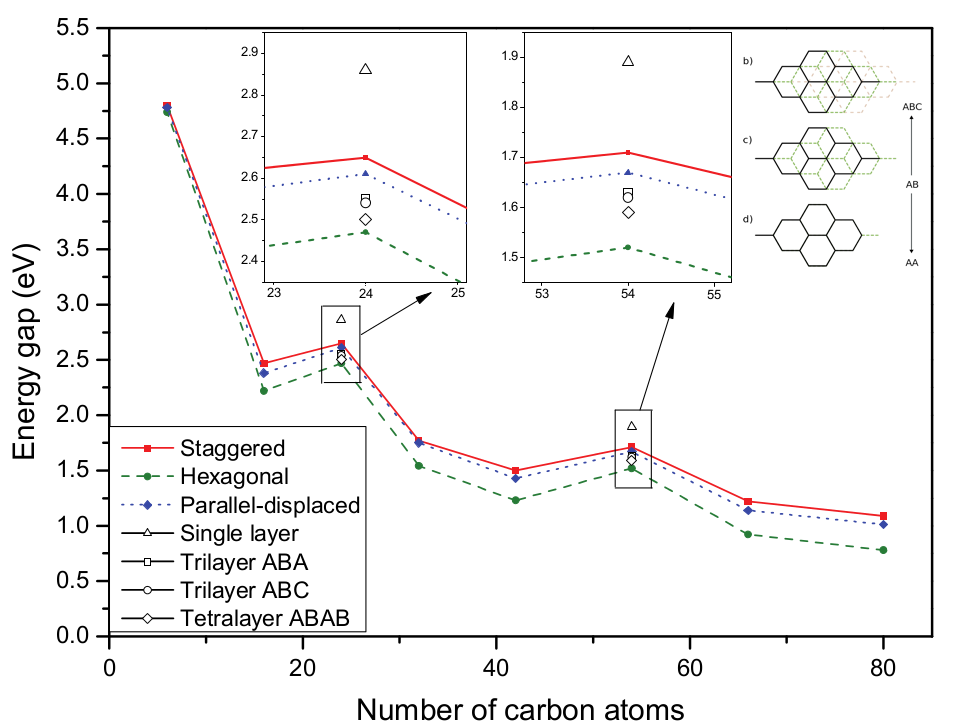
\includegraphics[width=0.9\textwidth]{figs/gap.png}

% {\footnotesize Variation of the energy gap with the size of graphene sheet
% model.\textsuperscript{ \ref{ft:fengJCP09}}}
% \end{center}
    
% \end{columns}
% \end{frame}


% %%%%%%%%%%%%%%%%%%%%%%%%%%%%%%%%%%%%%%%%%%%%%%%%%%%%%%%%%%%%%%%%%%%%%%%%%%%%%

% %%%%%%%%%%%%%%%%%%%%%%%
% \subsection{Synthesis}
% %%%%%%%%%%%%%%%%%%%%%%%

% \begin{frame}

% \vspace{-0.2cm}

% \noindent\makebox[\linewidth]{\rule{\linewidth}{0.4pt}}

% \vspace{-2.0mm}
% \begin{center}
% {\huge Synthesis of graphene}
% \end{center}

% \vspace{-6mm}
% \noindent\makebox[\linewidth]{\rule{\linewidth}{0.4pt}}

% \begin{columns}
% \column{0.51\textwidth}
% \begin{itemize}

% \item Exfoliation\footnote[frame]{\tiny A.K. Geim and K.S. Novoselov. Nature
% Materials, 6(3):183-191, 2007. \label{ft:geimNAT07}}

% \item Micromechanical cleavage
% \footnote[frame]{\tiny R.R. Nair, et al. Science, 320(5881):1308-1308, 2008.
% \label{ft:nairSC08}}


% \item Reduction of graphite oxide in dimethylformamide
% \footnote[frame]{\tiny S. Park, J. et al. Nano letters, 9(4):1593-1597, 2009.}

% \item Chemical Vapor Deposition
% \footnote[frame]{\tiny E. Rollings, et al. JPCS,
% 67(9-10):2172-2177, 2006.}

% \end{itemize}
% \column{0.6\textwidth}
% \begin{figure}
% \centering
% 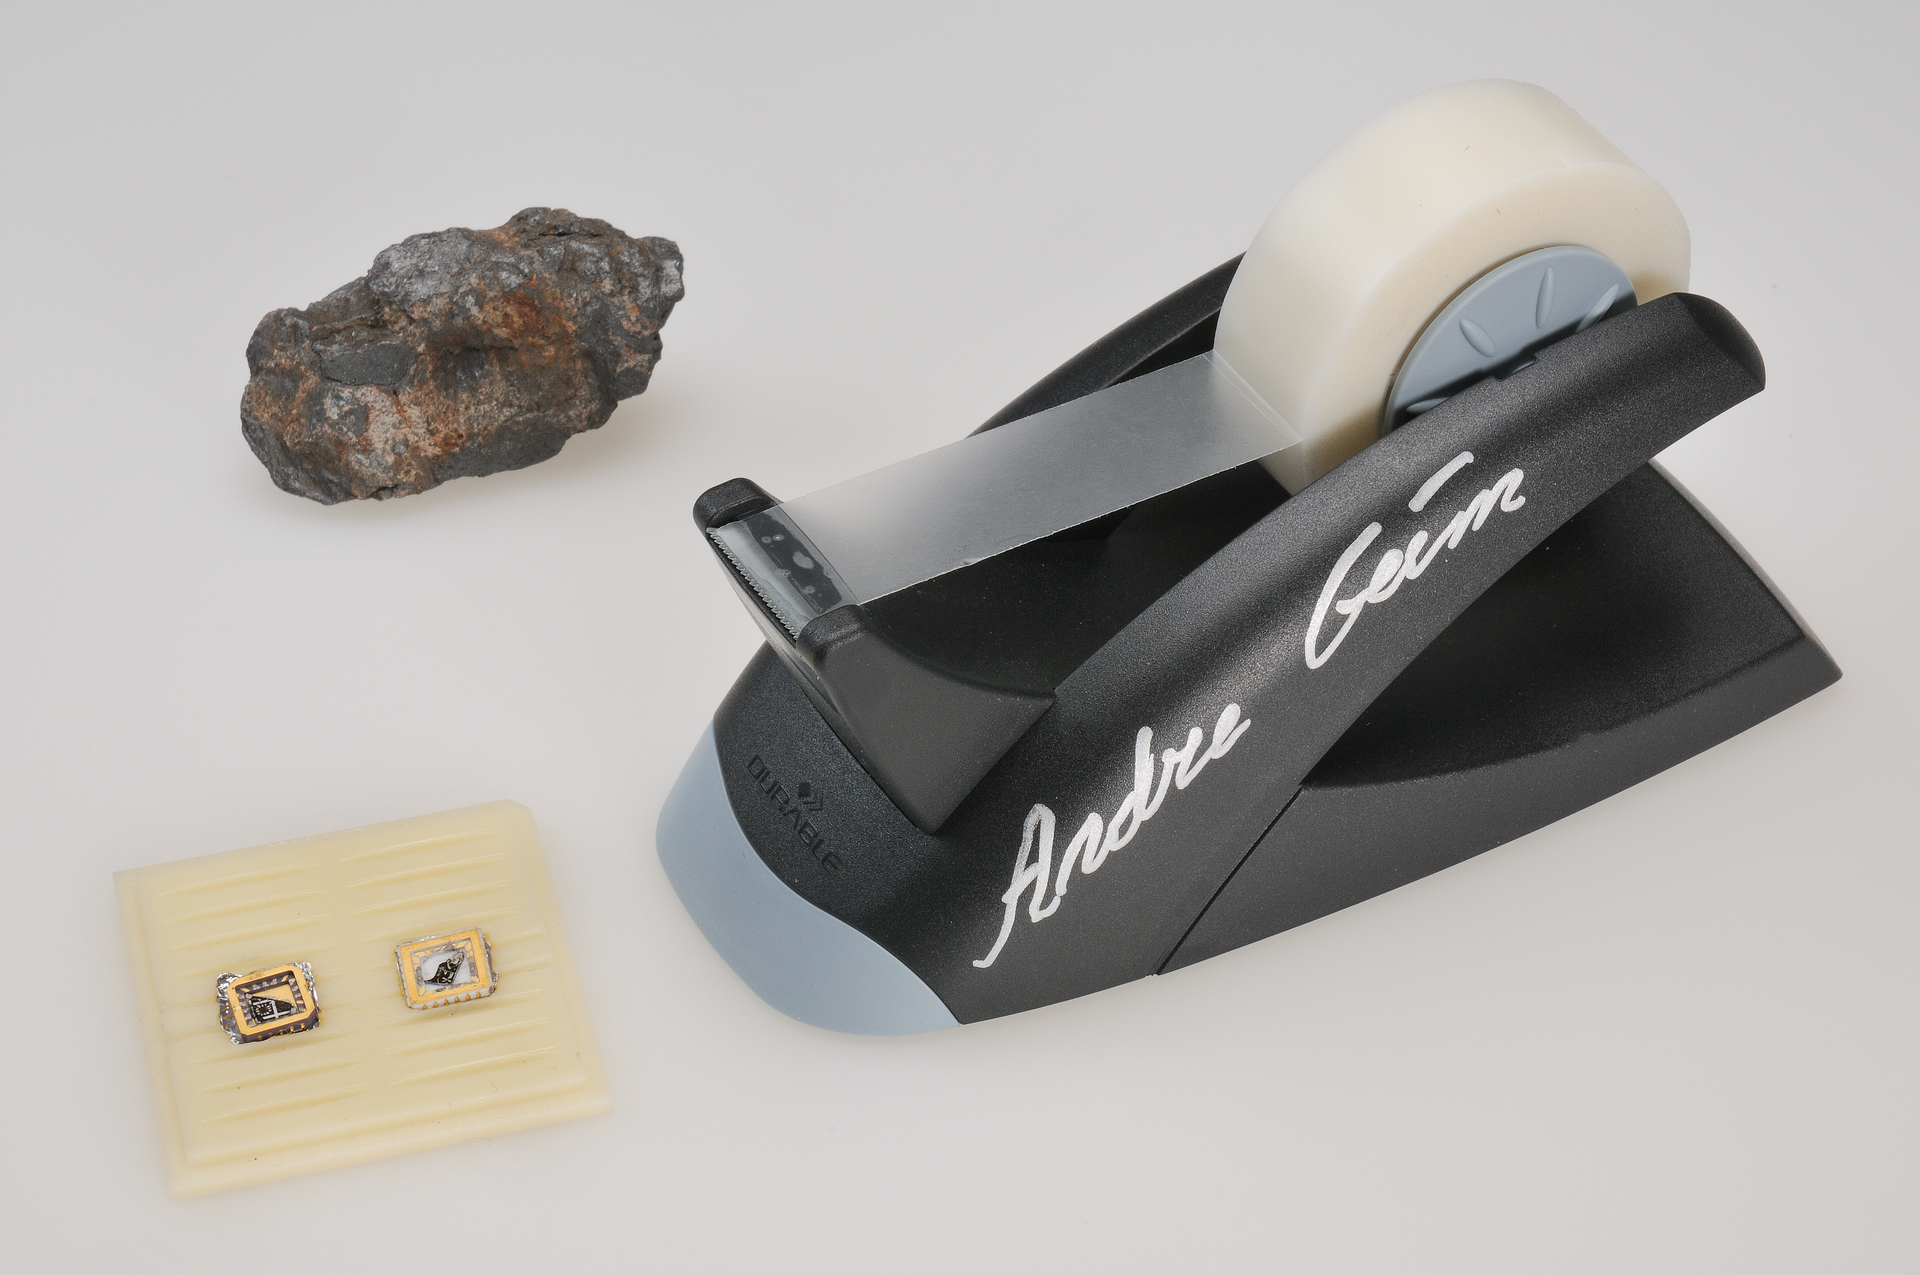
\includegraphics[width=0.75\textwidth]{figs/tools.png}

% {\scriptsize Graphite, a graphene transistor, and a tape dispenser donated to
% the Nobel Museum.}\footnote[frame]{\tiny By
% Gabriel Hildebrand - Nobelmuseet, Public Domain.}
% \end{figure}

% \end{columns}

% \hspace{5mm}

% \end{frame}

% %%%%%%%%%%%%%%%%%%%%%%%%%%%%%%%%%%%%%%%%%%%%%%%%%%%%%%%%%%%%%%%%%%%%%%%%%%%%%

% % %%%%%%%%%%%%%%%%%%%%%%%
% % \subsection{Characterization}
% % %%%%%%%%%%%%%%%%%%%%%%%

% % \begin{frame}

% % \vspace{-0.7cm}

% % \noindent\makebox[\linewidth]{\rule{\linewidth}{0.4pt}}

% % \vspace{-2.0mm}
% % \begin{center}
% % {\huge Characterization of graphene}
% % \end{center}

% % \vspace{-6mm}
% % \noindent\makebox[\linewidth]{\rule{\linewidth}{0.4pt}}

% % % \vfill

% % \begin{columns}
% % \column{0.6\textwidth}
% % 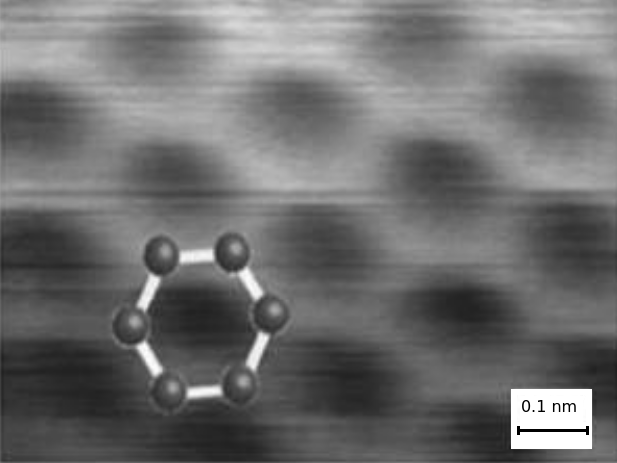
\includegraphics[width=0.75\textwidth]{figs/tem.png}

% % Transmission electron microscopy of graphene.\textsuperscript{
% % \ref{ft:stolyarovaPNAS07}}
% % \end{figure}
% % \column{0.5\textwidth}
% % \begin{itemize}

% % \item Scanning Tunneling Microscopy\textsuperscript{ \ref{ft:geimNAT07}}

% % \item Raman Spectroscopy\textsuperscript{ \ref{ft:geimNAT07}}

% % \item Atomic force microscopy
% % \footnote[frame]{\tiny K.S. Novoselov, A.K. Geim, et. al. Science,
% % 306(5696):666-669, 2004}

% % \item Transmission Electron Microscopy
% % \footnote[frame]{\tiny E. Stolyarova, et al. PNAS, 104(22):9209, 2007. \label{ft:stolyarovaPNAS07}}

% % \end{itemize}
% % \end{columns}

% % \hspace{5mm}

% % \end{frame}



% %%%%%%%%%%%%%%%%%%%%%%%%%%%%%%%%%%%%%%%%%%%%%%%%%%%%%%%%%%%%%%%%%%%%%%%%%%%%%

% \begin{frame}

% \begin{columns}

% \column{0.3\textwidth}

% \begin{center}
% 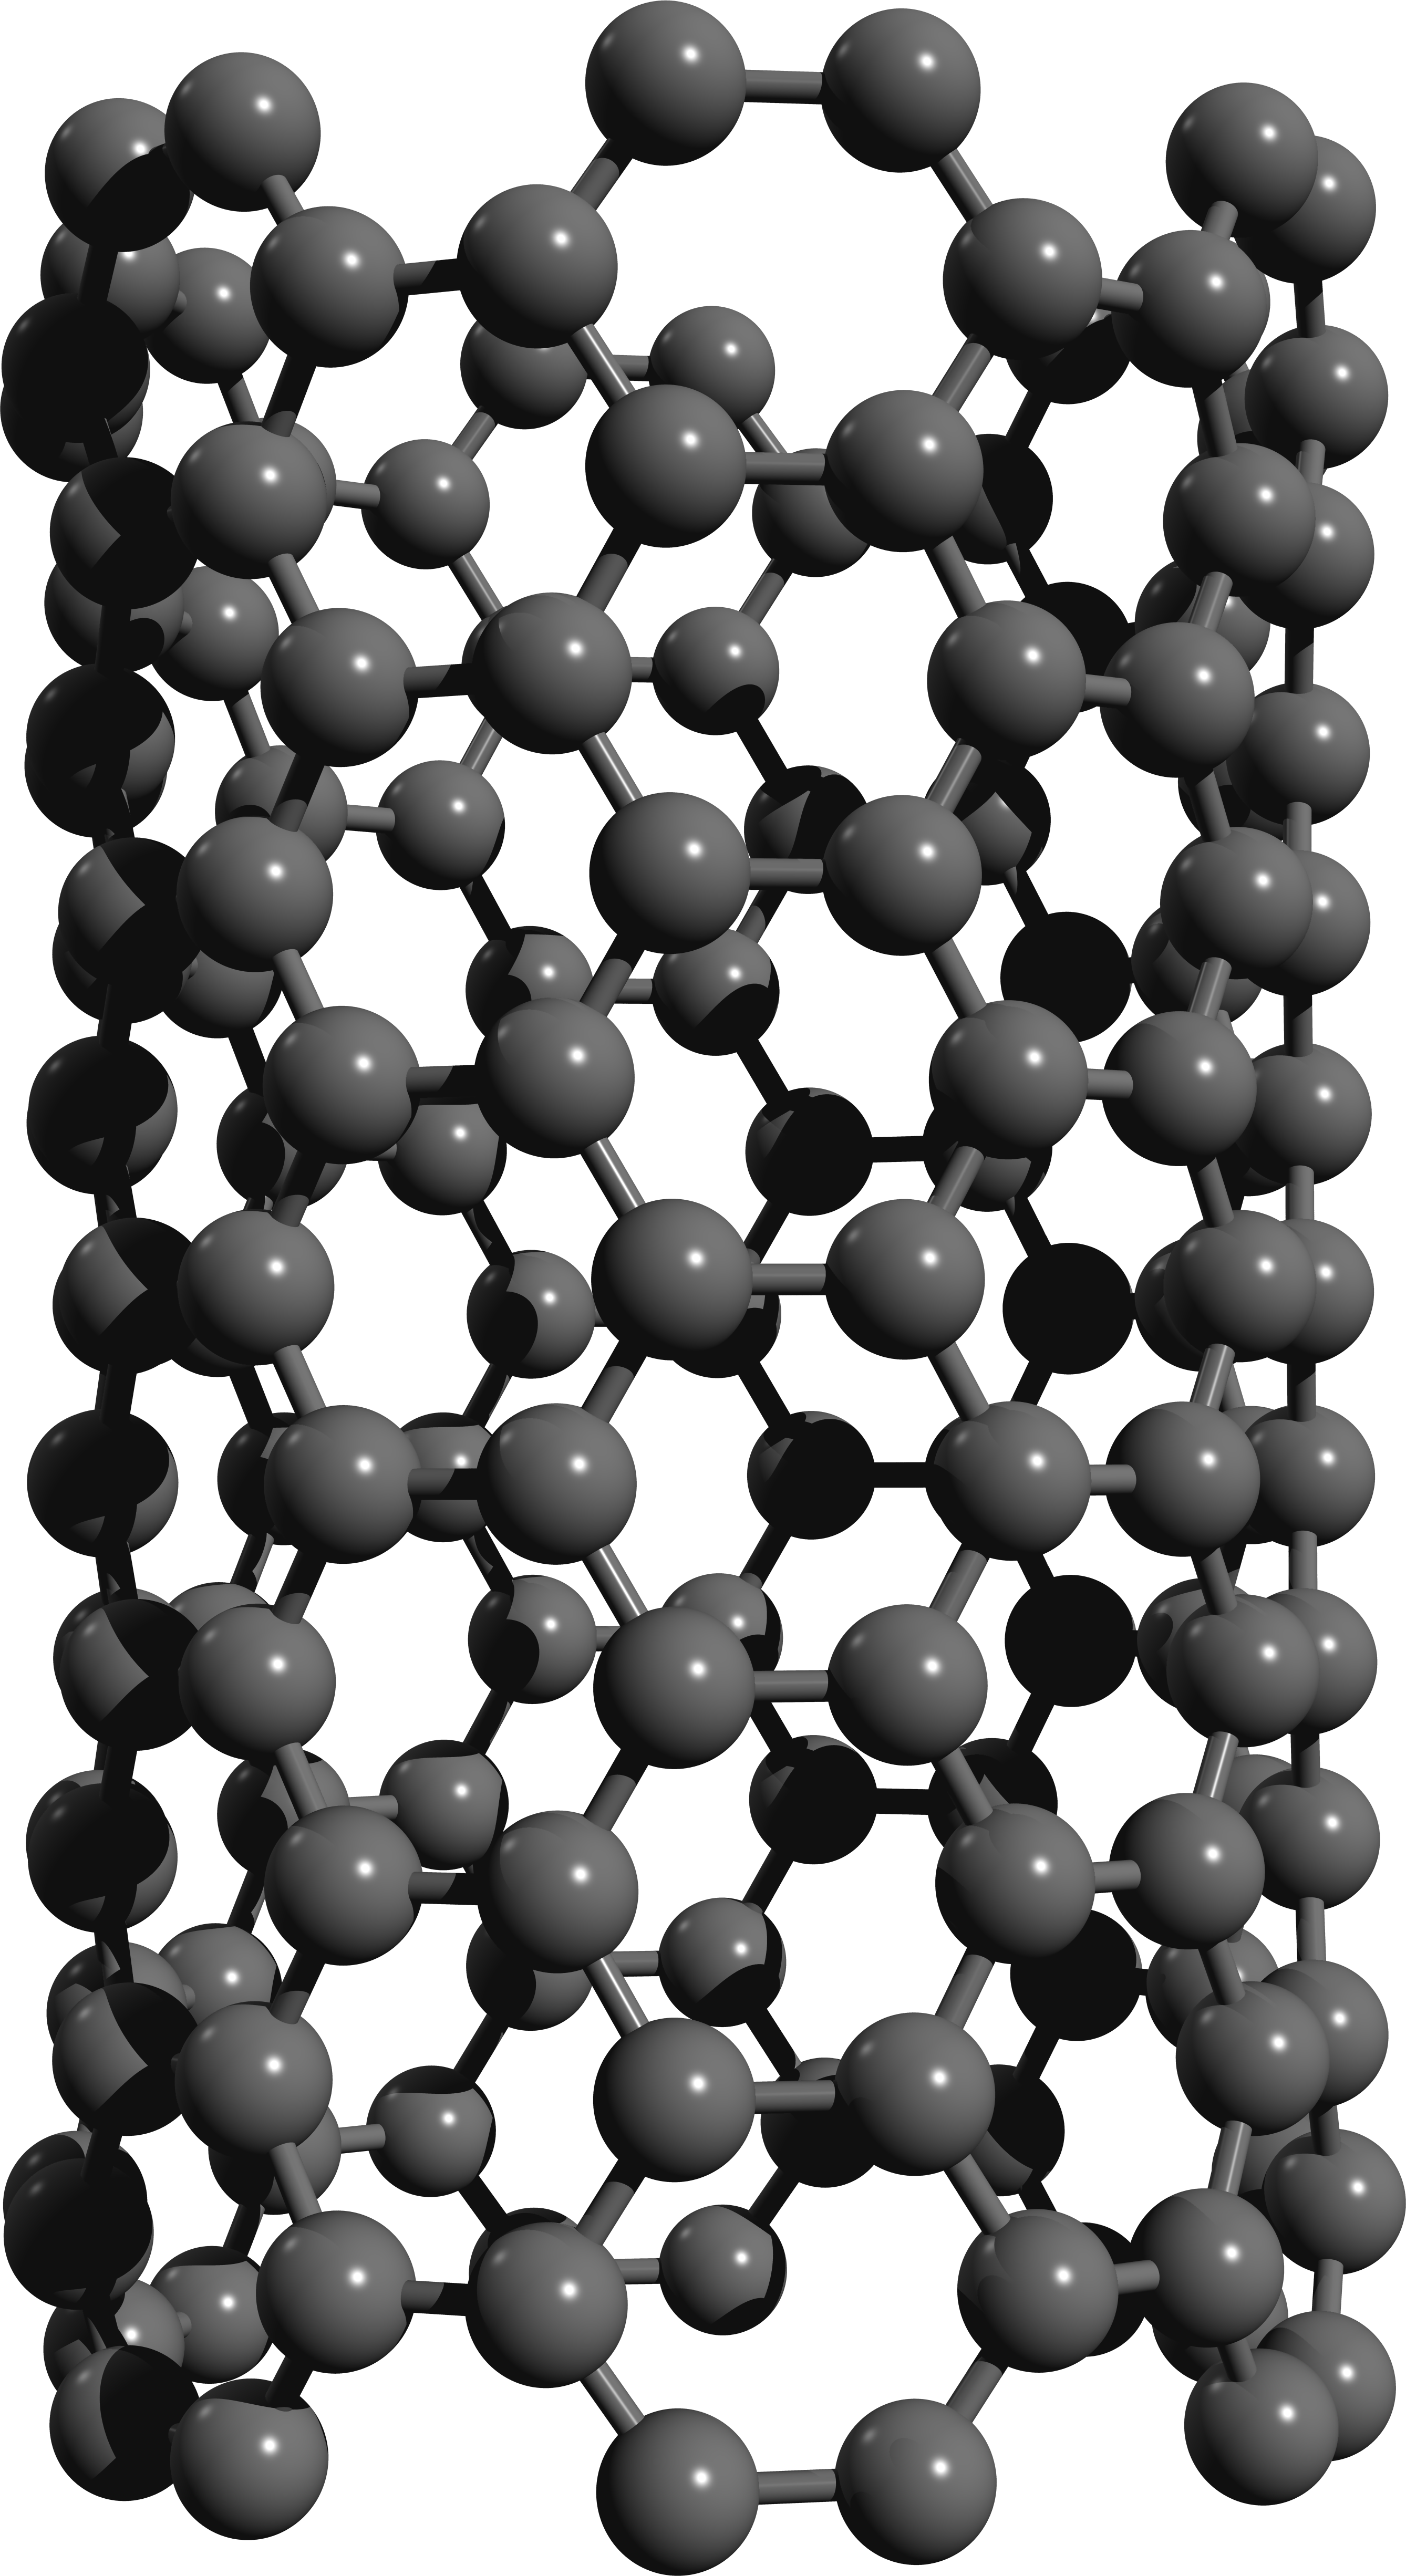
\includegraphics[width=0.9\textwidth]{figs/nanotube2.png}\\

% \vspace{3mm}
% Carbon nanotube
% \end{center}

% \column{0.7\textwidth}
% \begin{center}
% 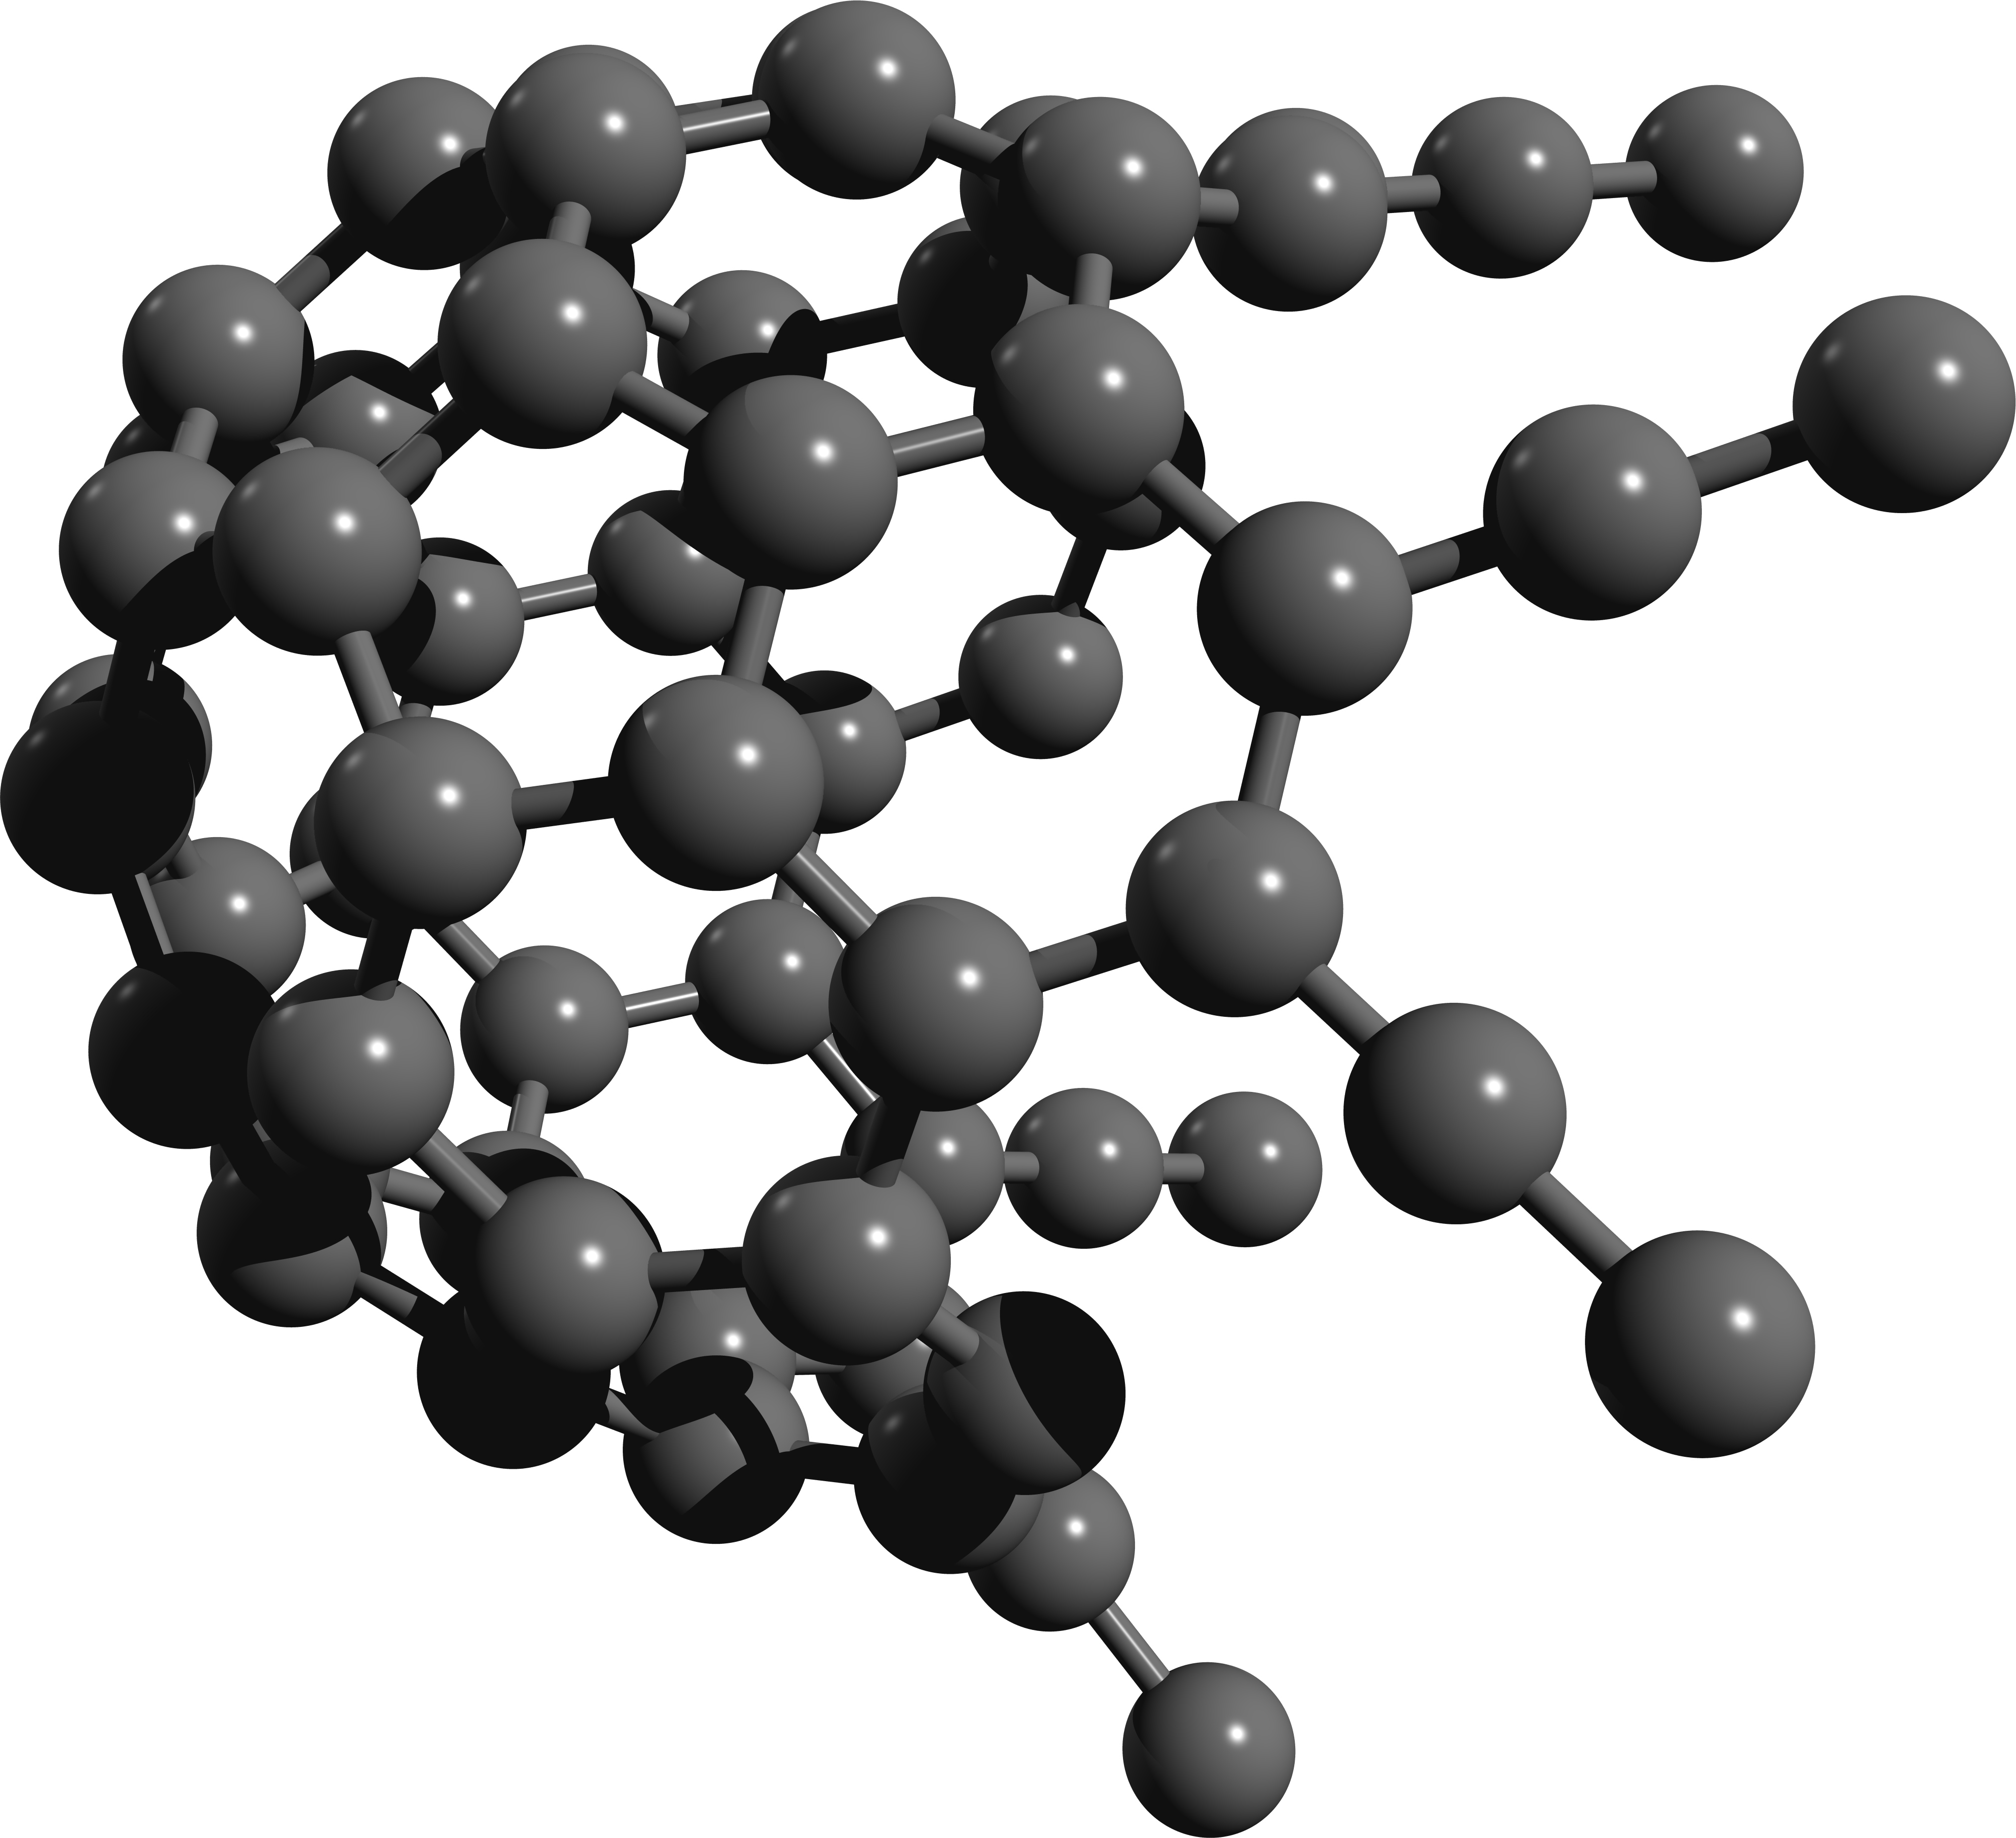
\includegraphics[width=0.35\textwidth]{figs/fullerene2.png} 
% \hspace{5mm}
% 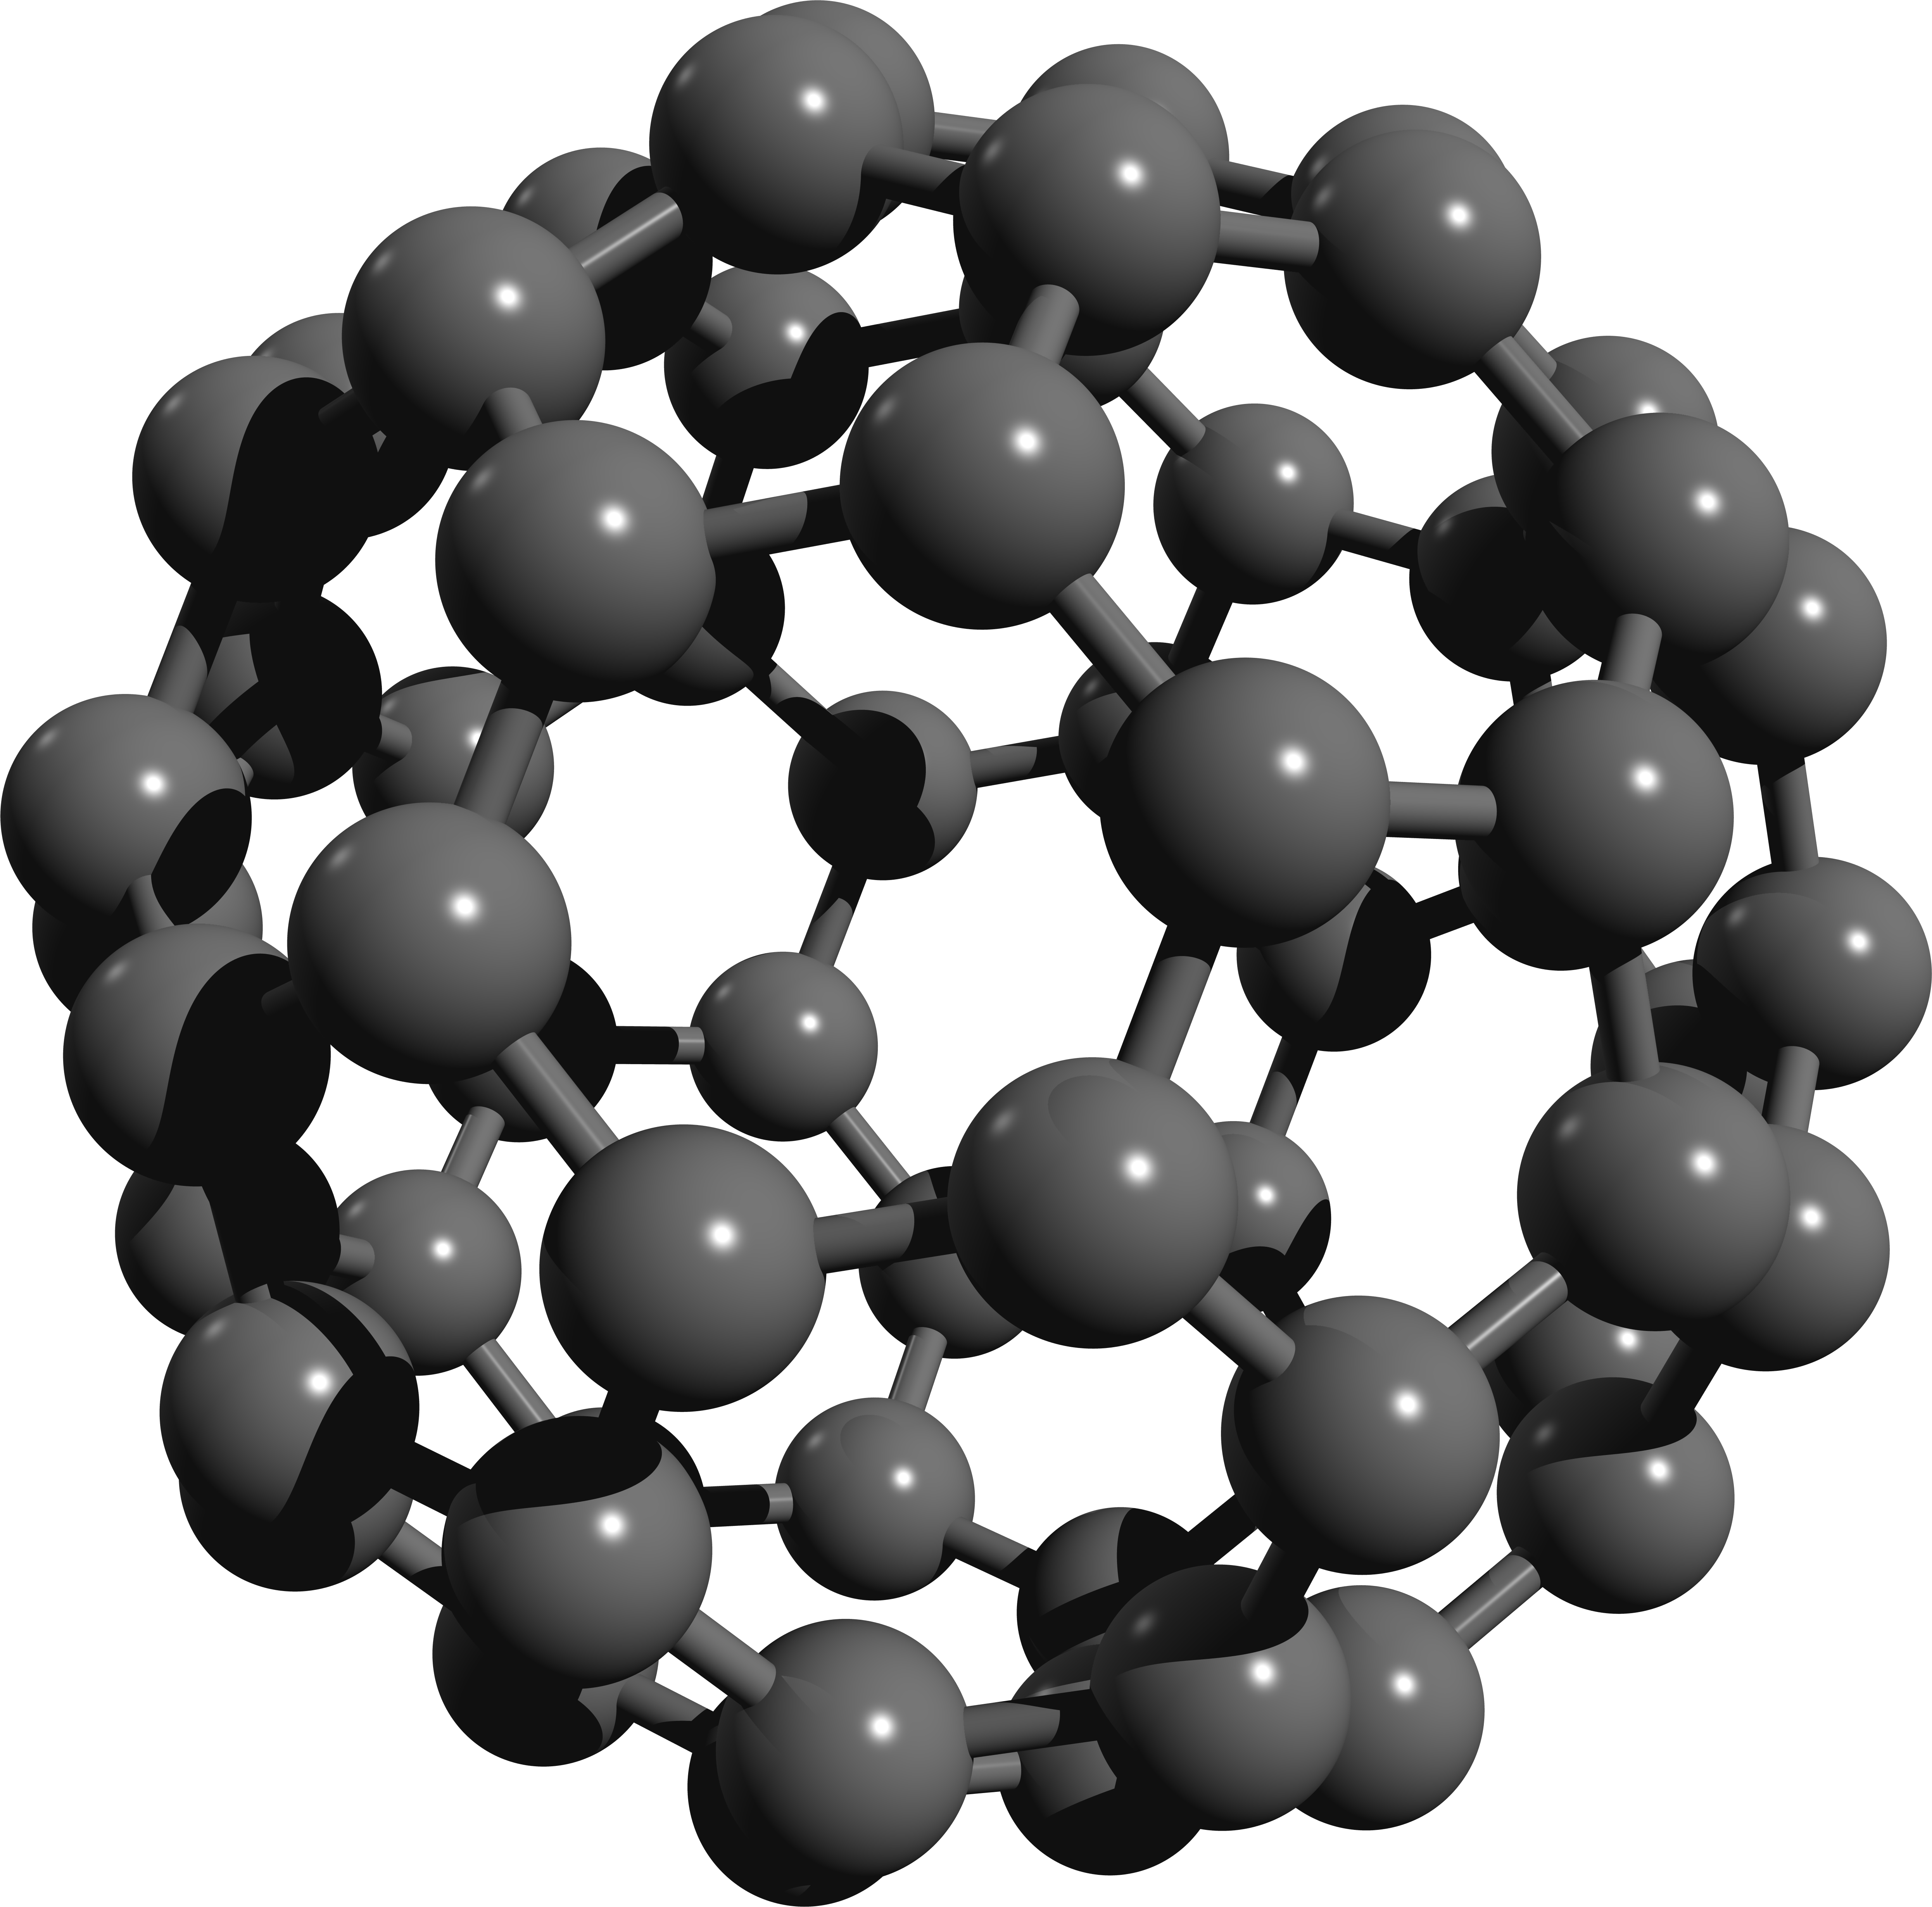
\includegraphics[width=0.35\textwidth]{figs/fullerene1.png}\\
% Fullerene

% \vspace{5mm}
% 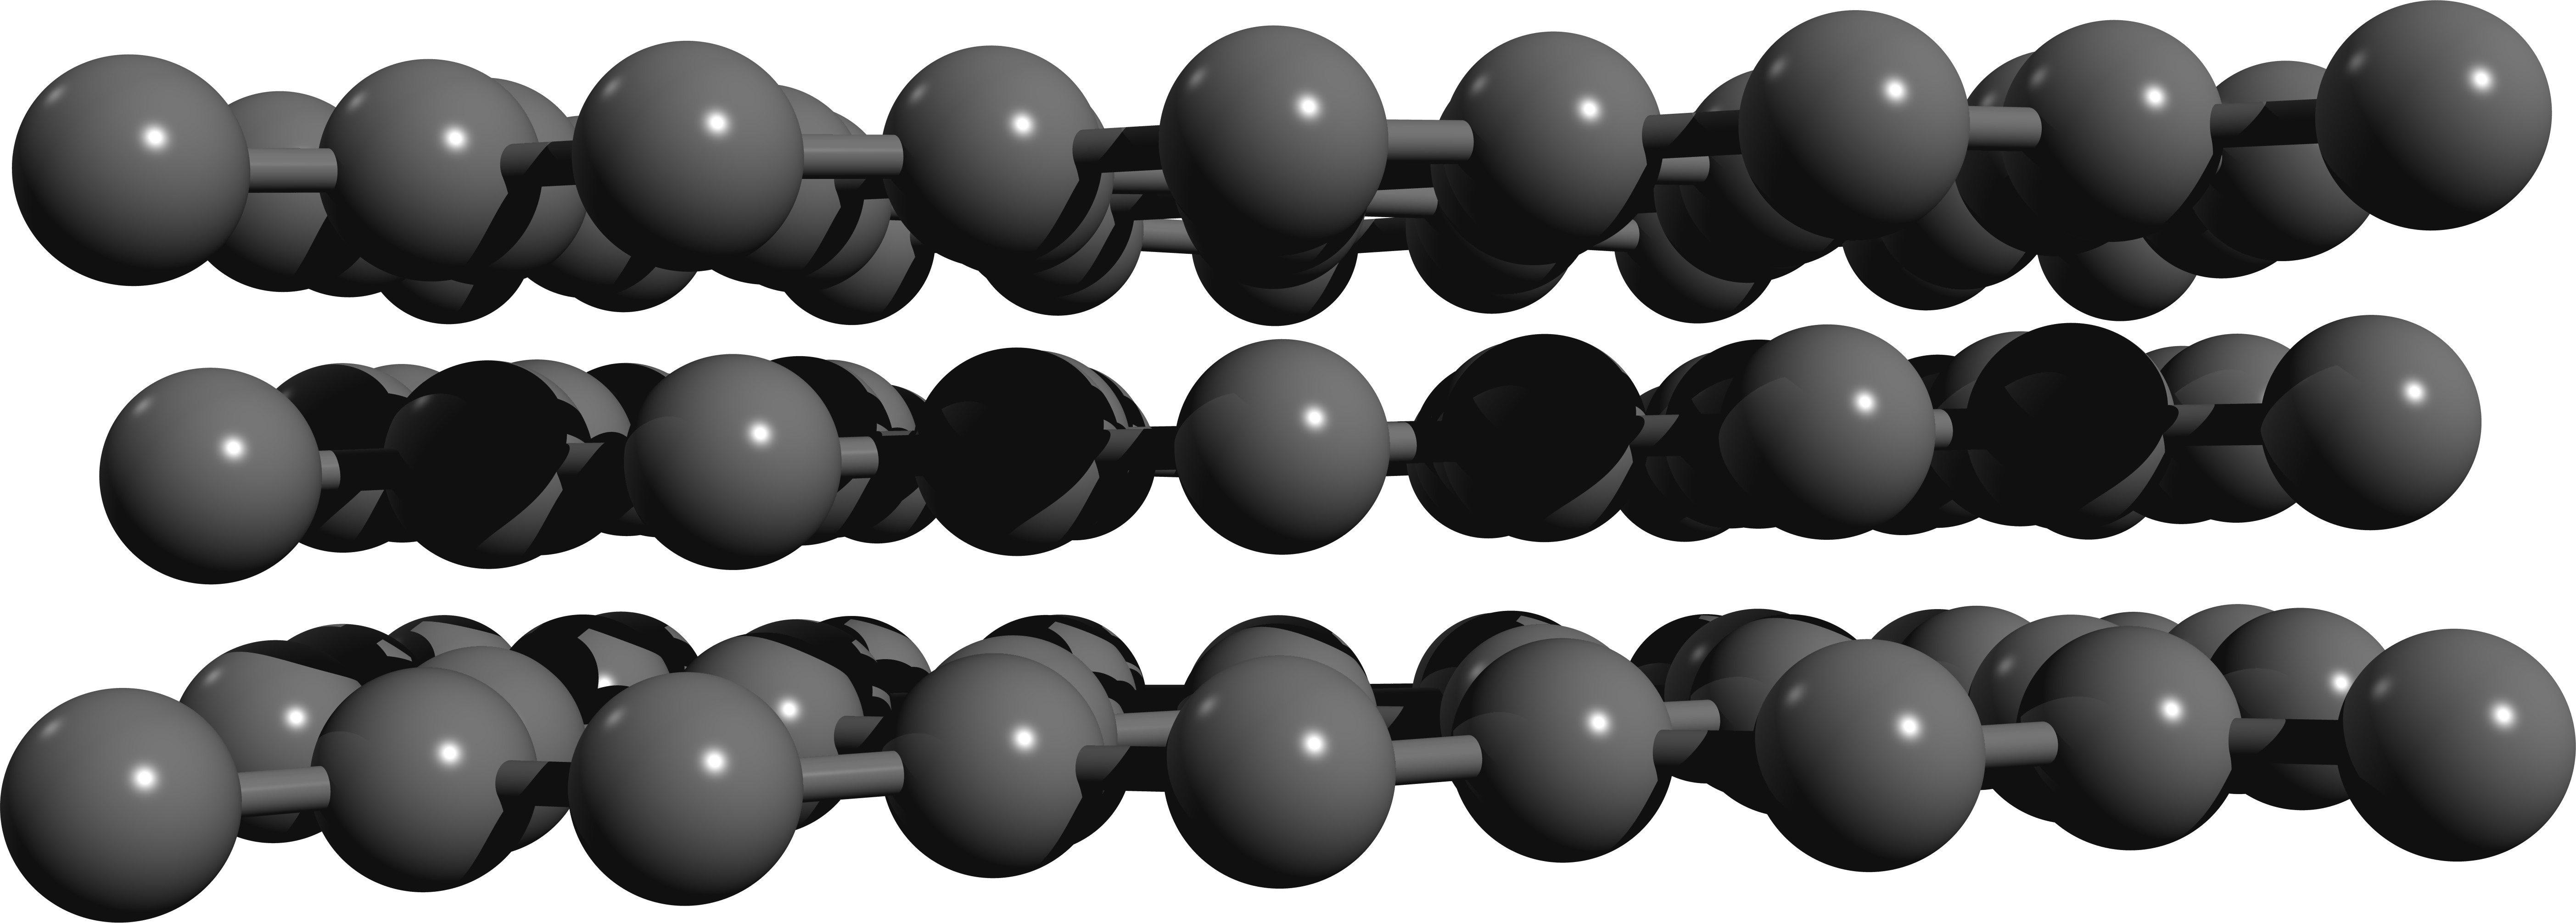
\includegraphics[width=0.35\textwidth]{figs/graphite2.png} 
% \vspace{2mm} \hspace{5mm}
% 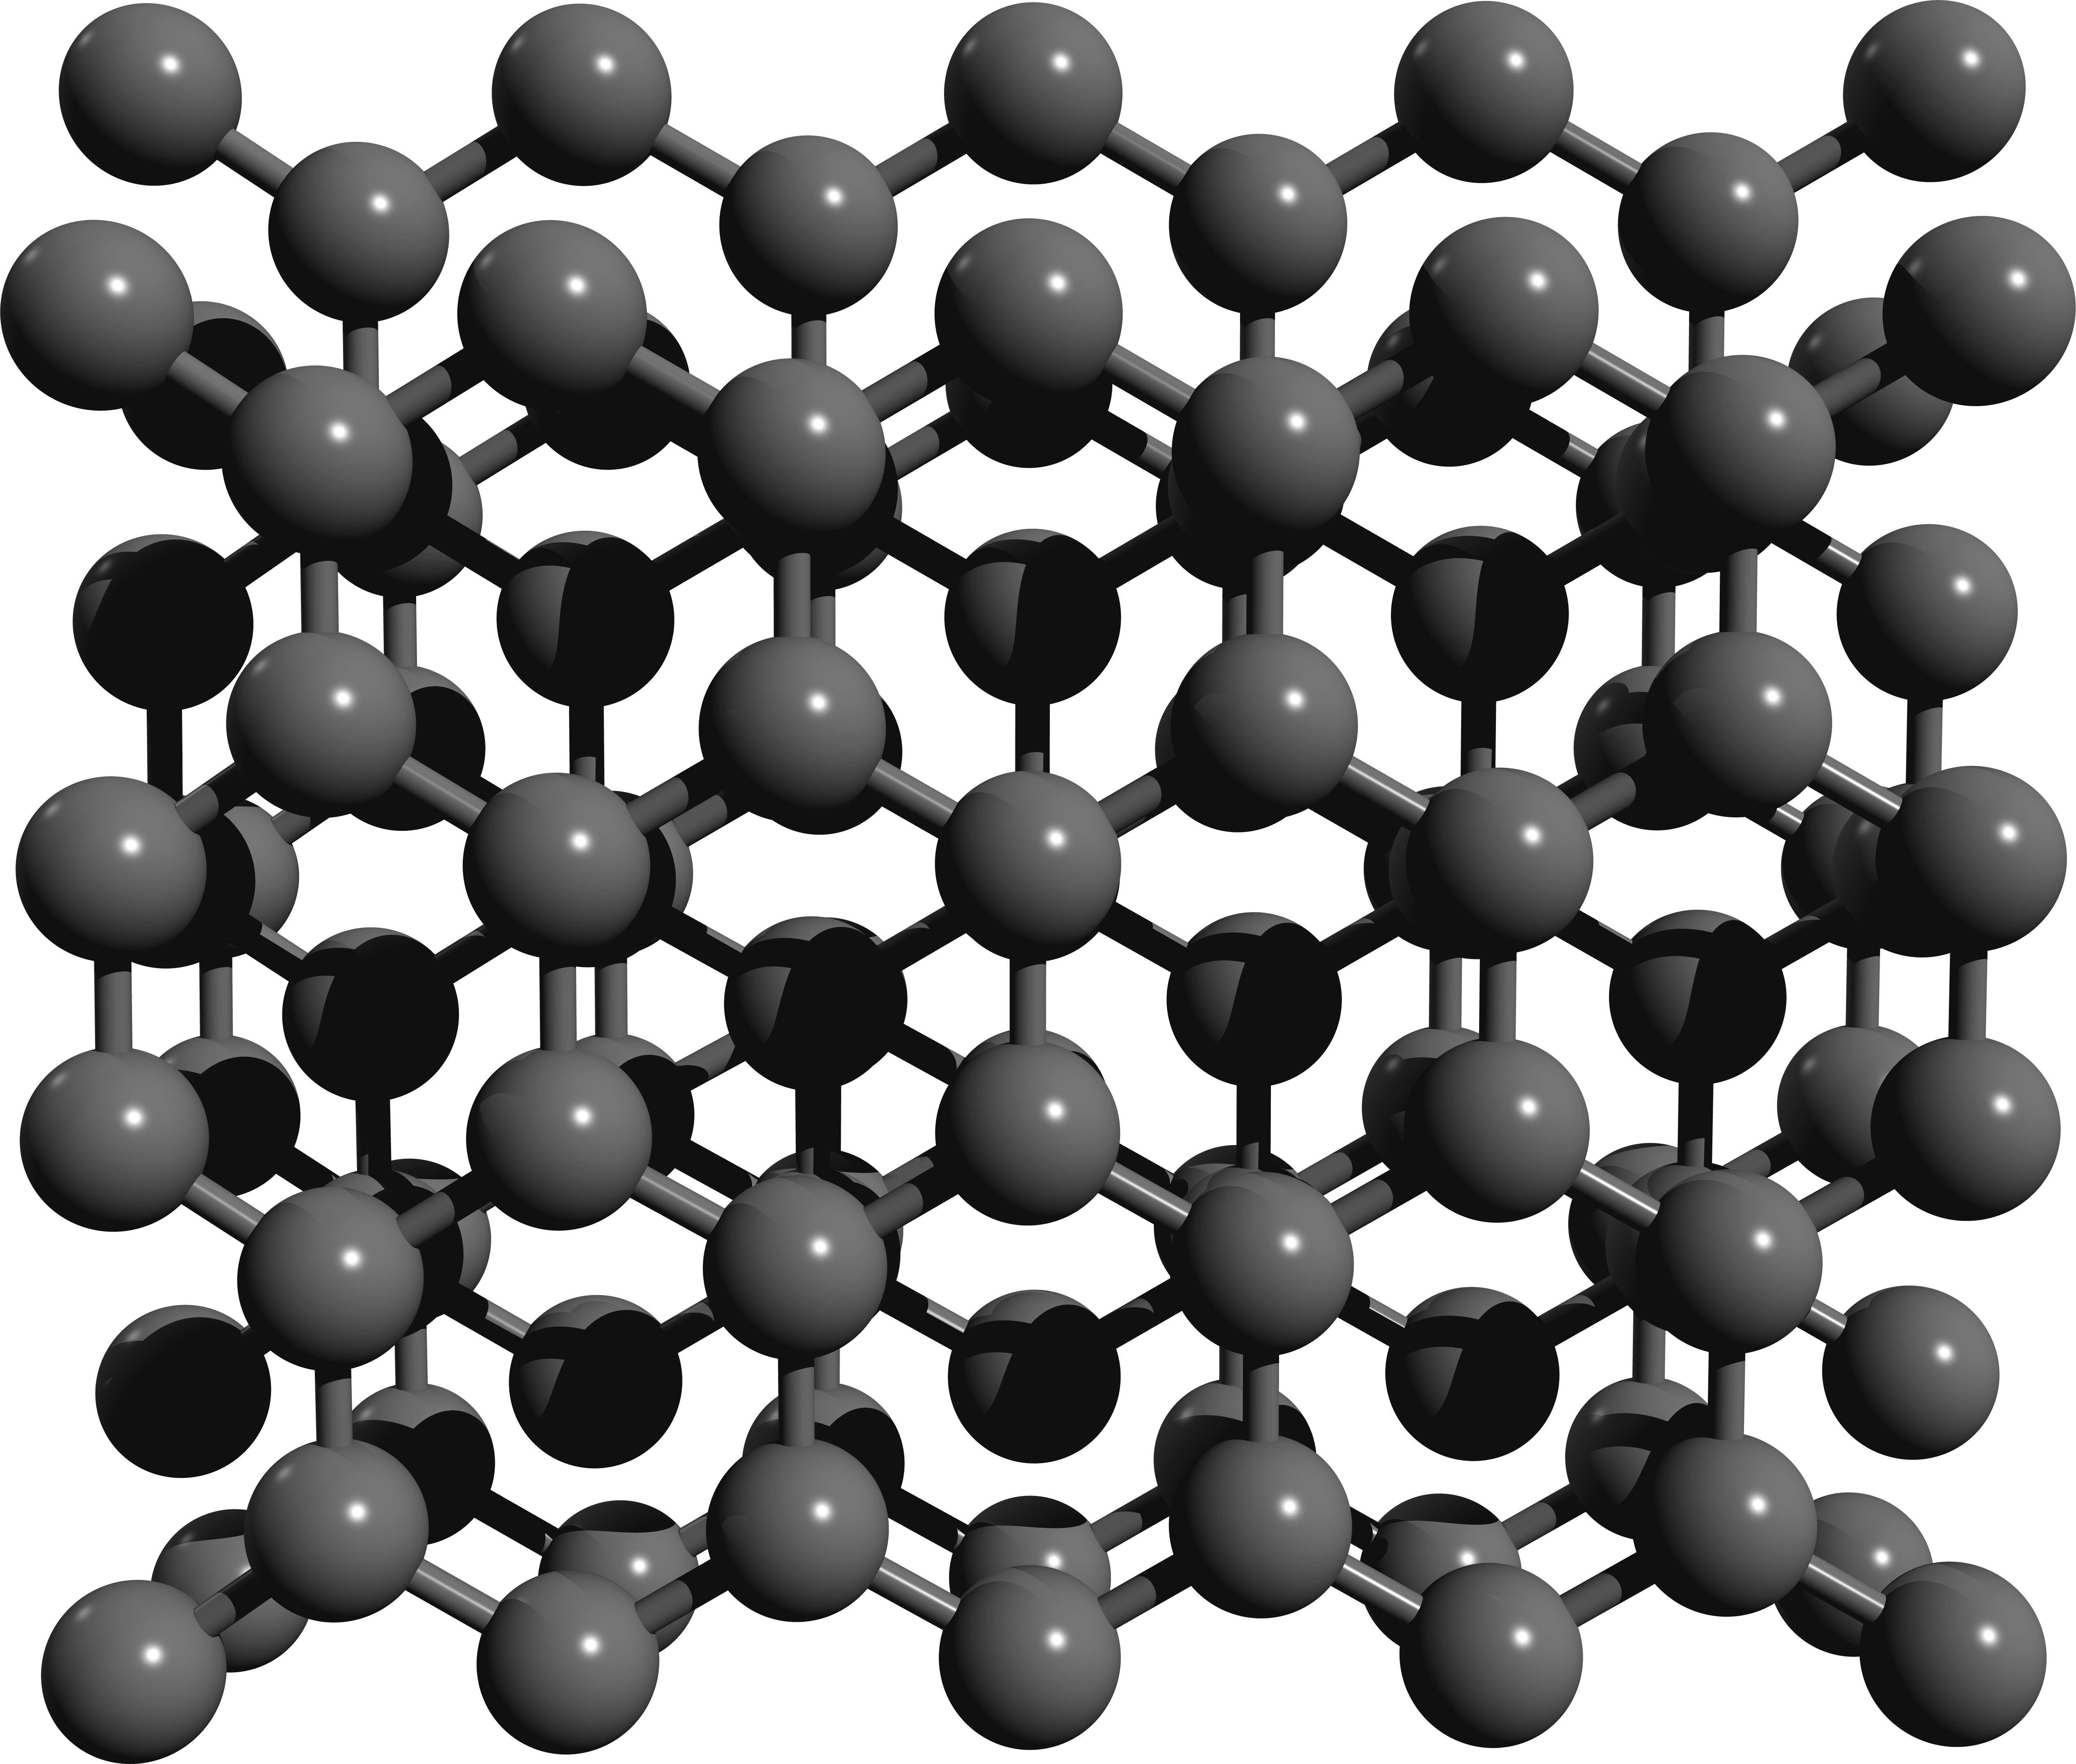
\includegraphics[width=0.35\textwidth]{figs/graphite1.png}\\
% Graphite

% \end{center}

% \end{columns}

% \vspace{3mm}
% \begin{center}
% {\huge Structures obtained from graphene}
% \end{center}

% \end{frame}

% %%%%%%%%%%%%%%%%%%%%%%%%%%%%%%%%%%%%%%%%%%%%%%%%%%%%%%%%%%%%%%%%%%%%%%%%%%%%%


% %%%%%%%%%%%%%%%%%%%%%%%
% \subsection{Functionalization}
% %%%%%%%%%%%%%%%%%%%%%%%

% \begin{frame}

% \begin{columns}

% \column{0.5\textwidth}

% \begin{center}
% 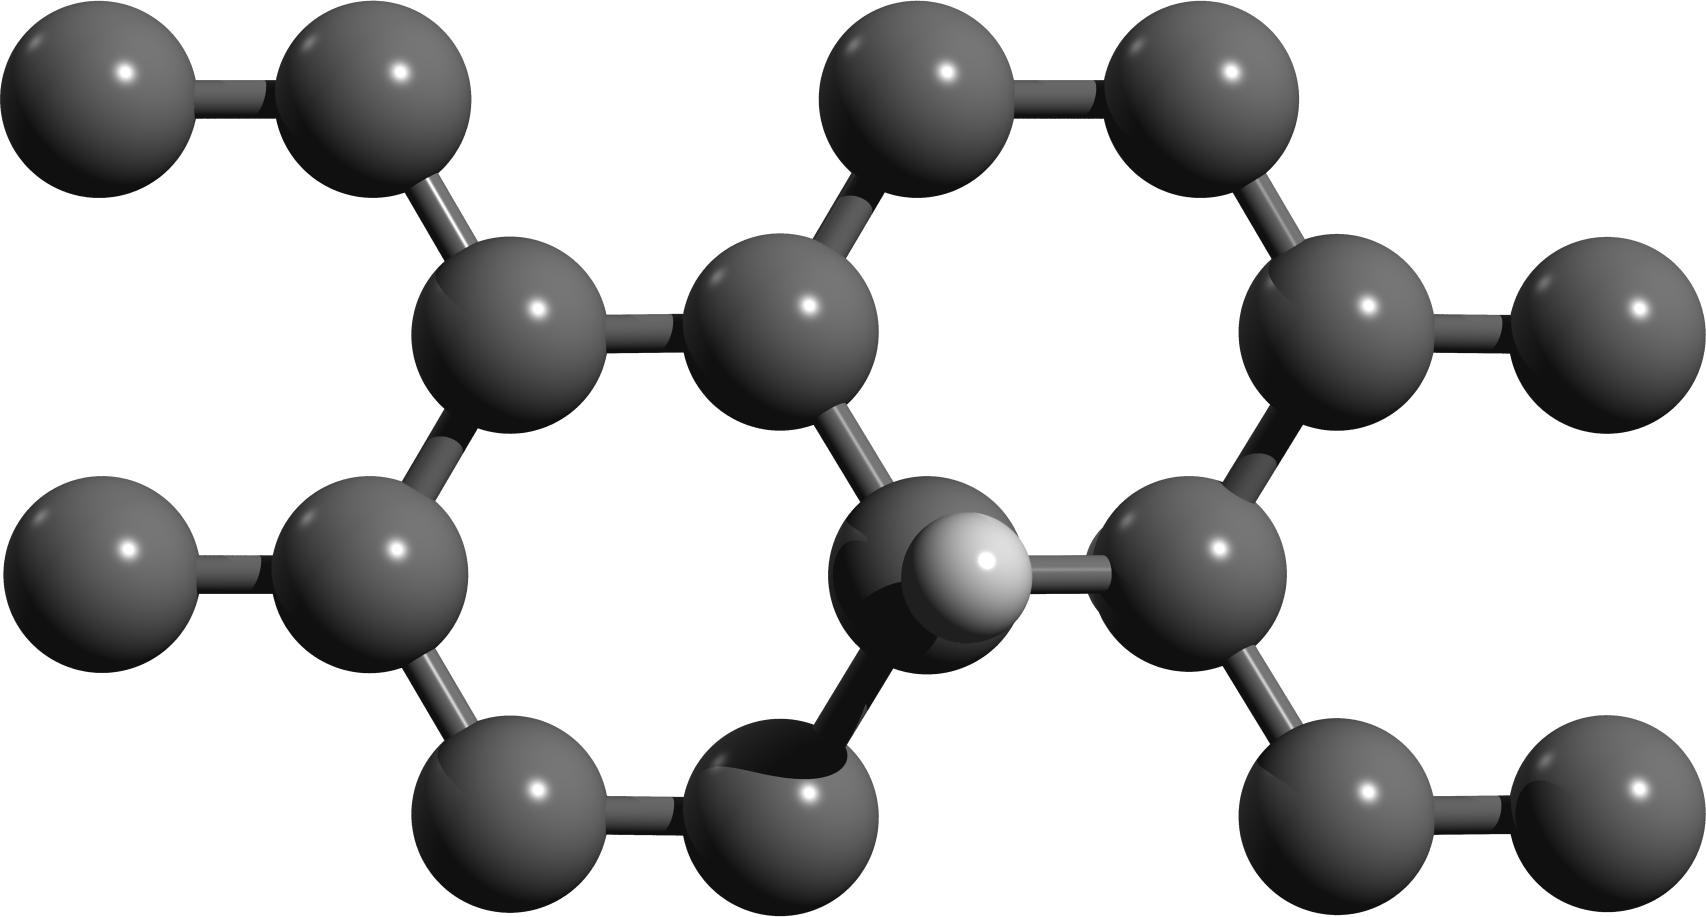
\includegraphics[width=0.8\textwidth]{figs/row.png}\\
% % {\small 12.5\% of hydrogenation}

% \vspace{7mm}
% 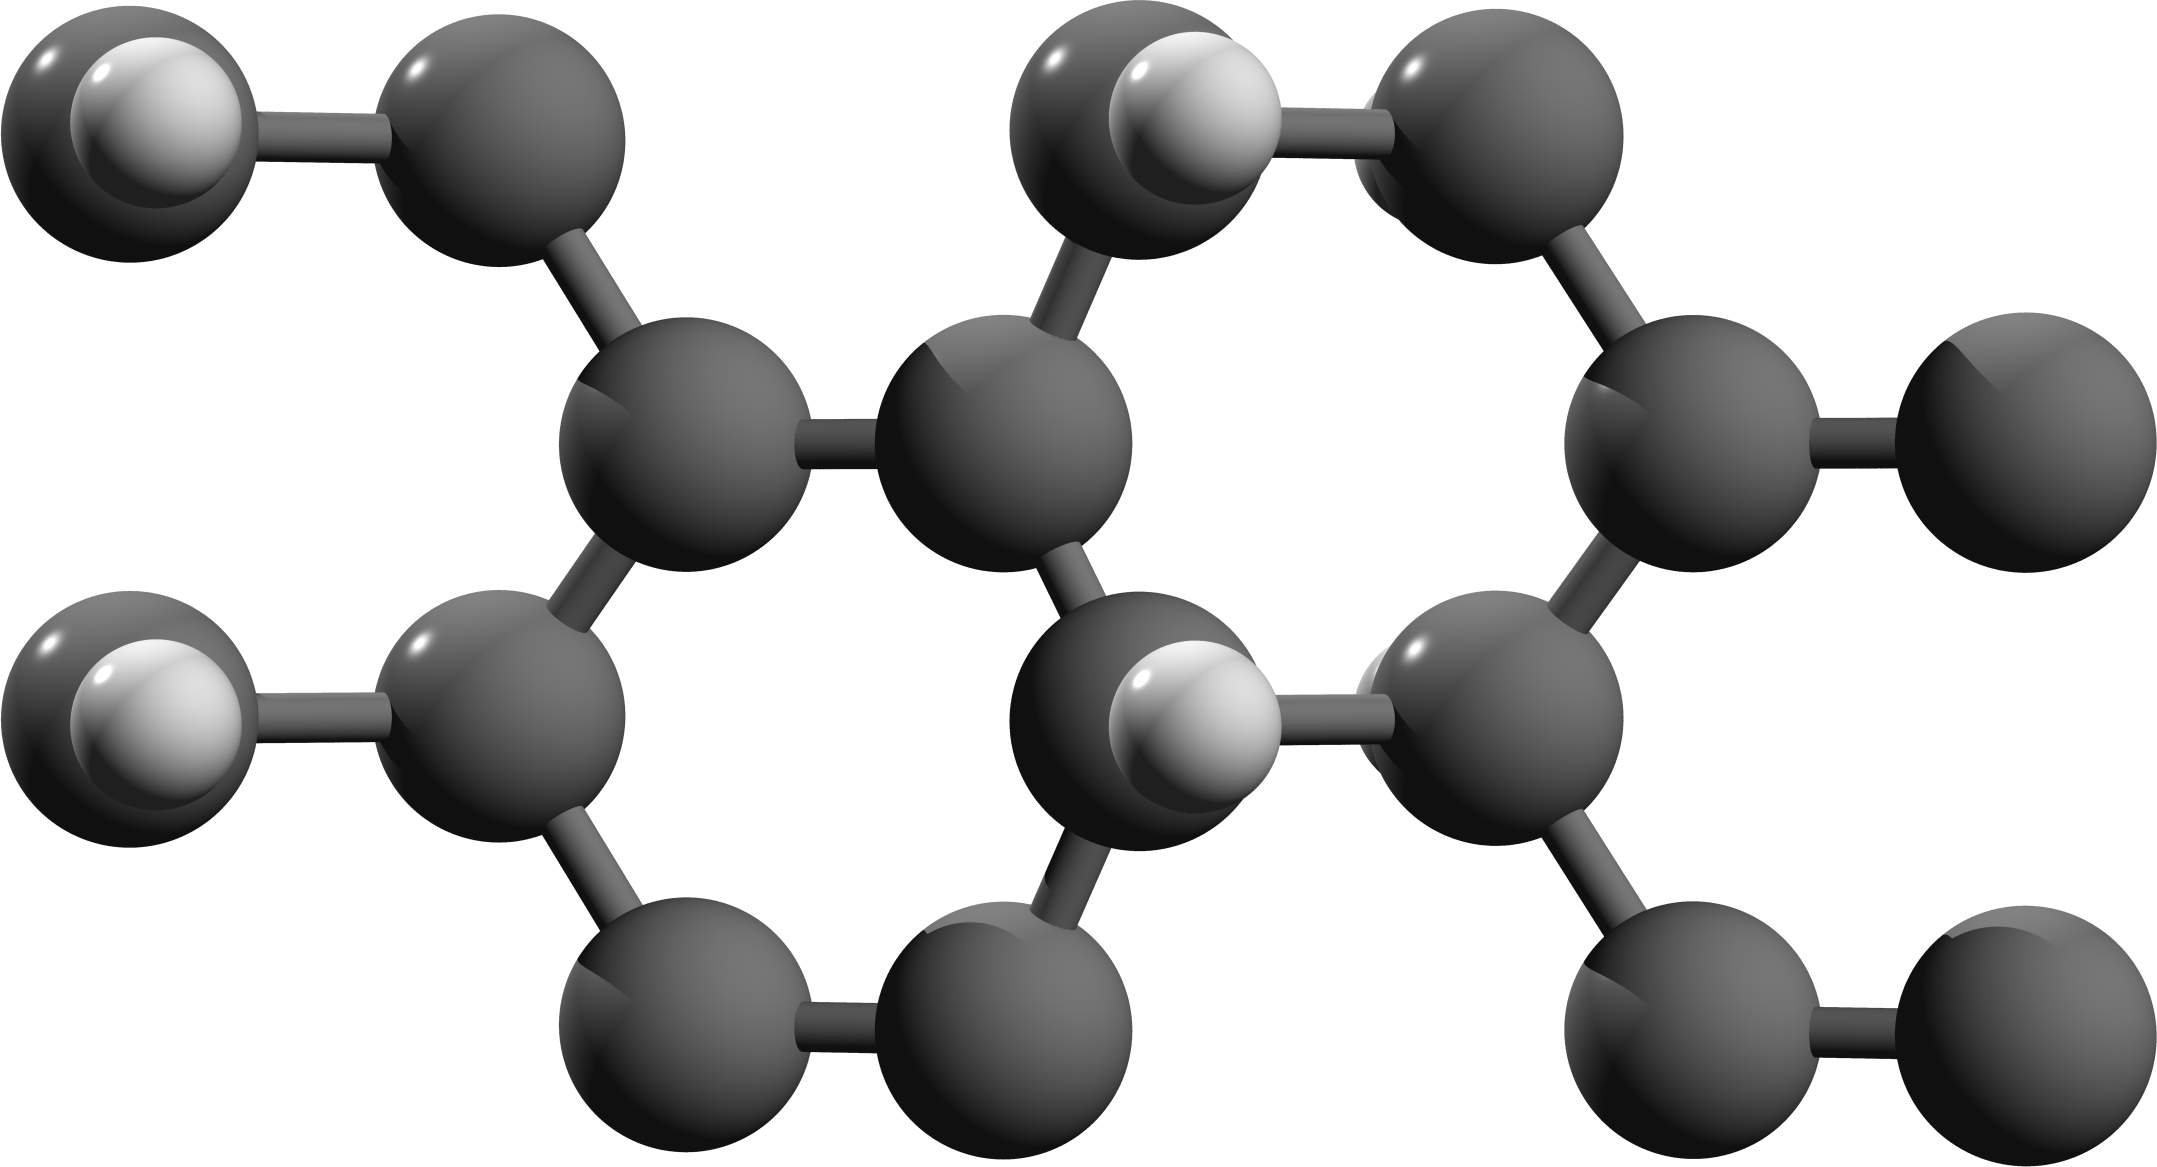
\includegraphics[width=0.8\textwidth]{figs/alt1.png}\\
% % {\small 50\% of hydrogenation}


% \vspace{5mm}
% \end{center}

% \column{0.5\textwidth}

% \centering
% \begin{center}
% 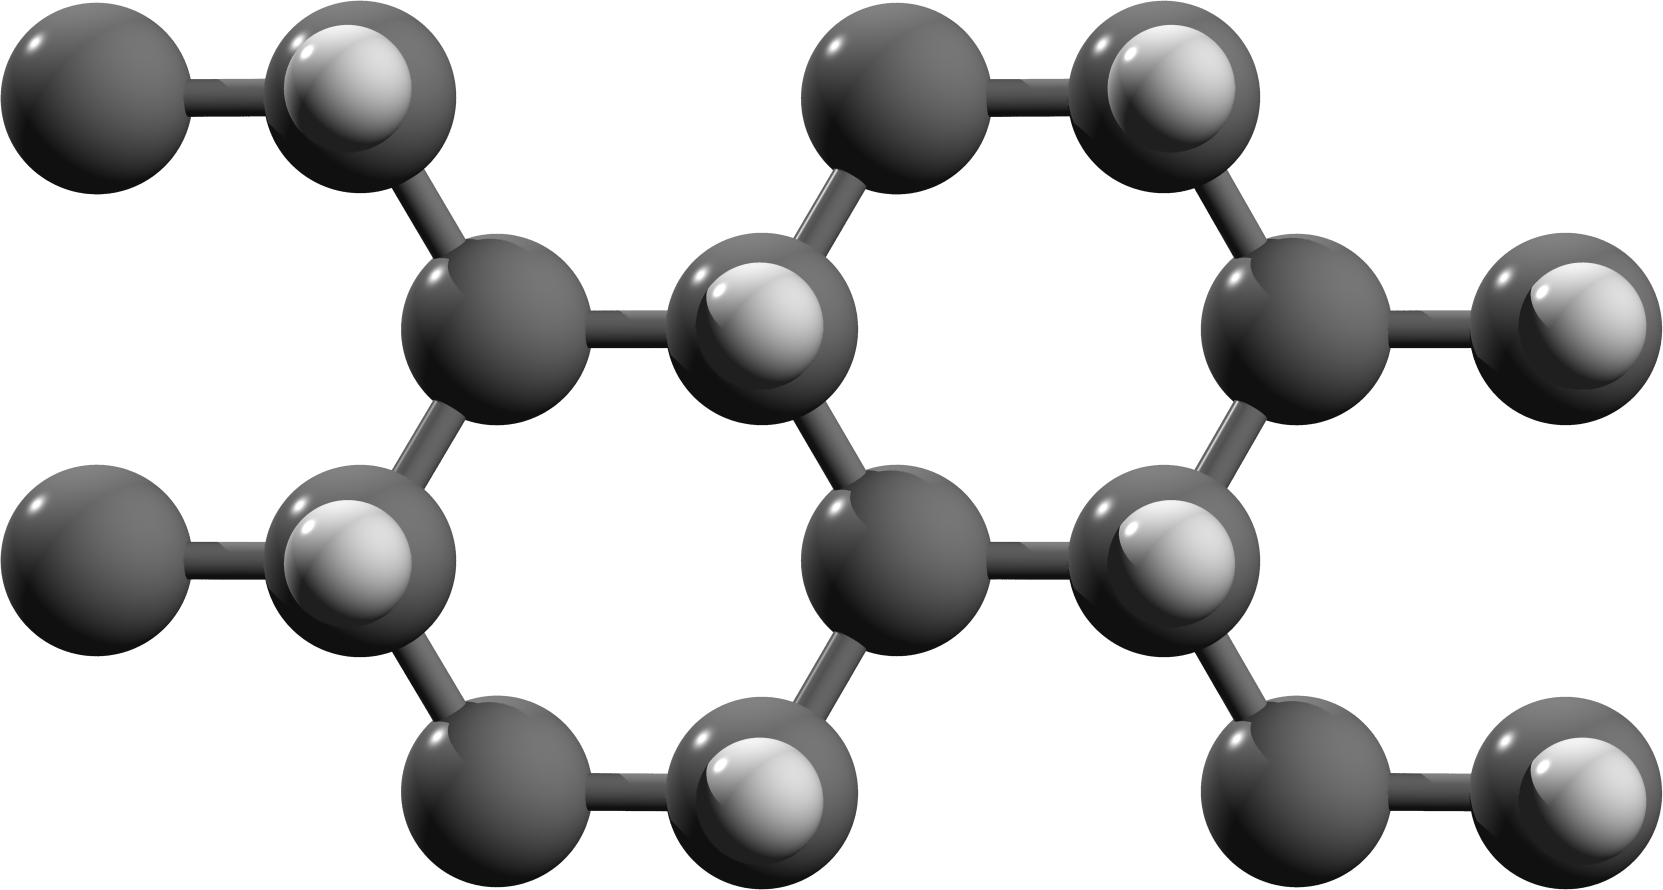
\includegraphics[width=0.8\textwidth]{figs/up1.png}\\
% % {\small 50\% of hydrogenation}

% \vspace{7mm}
% 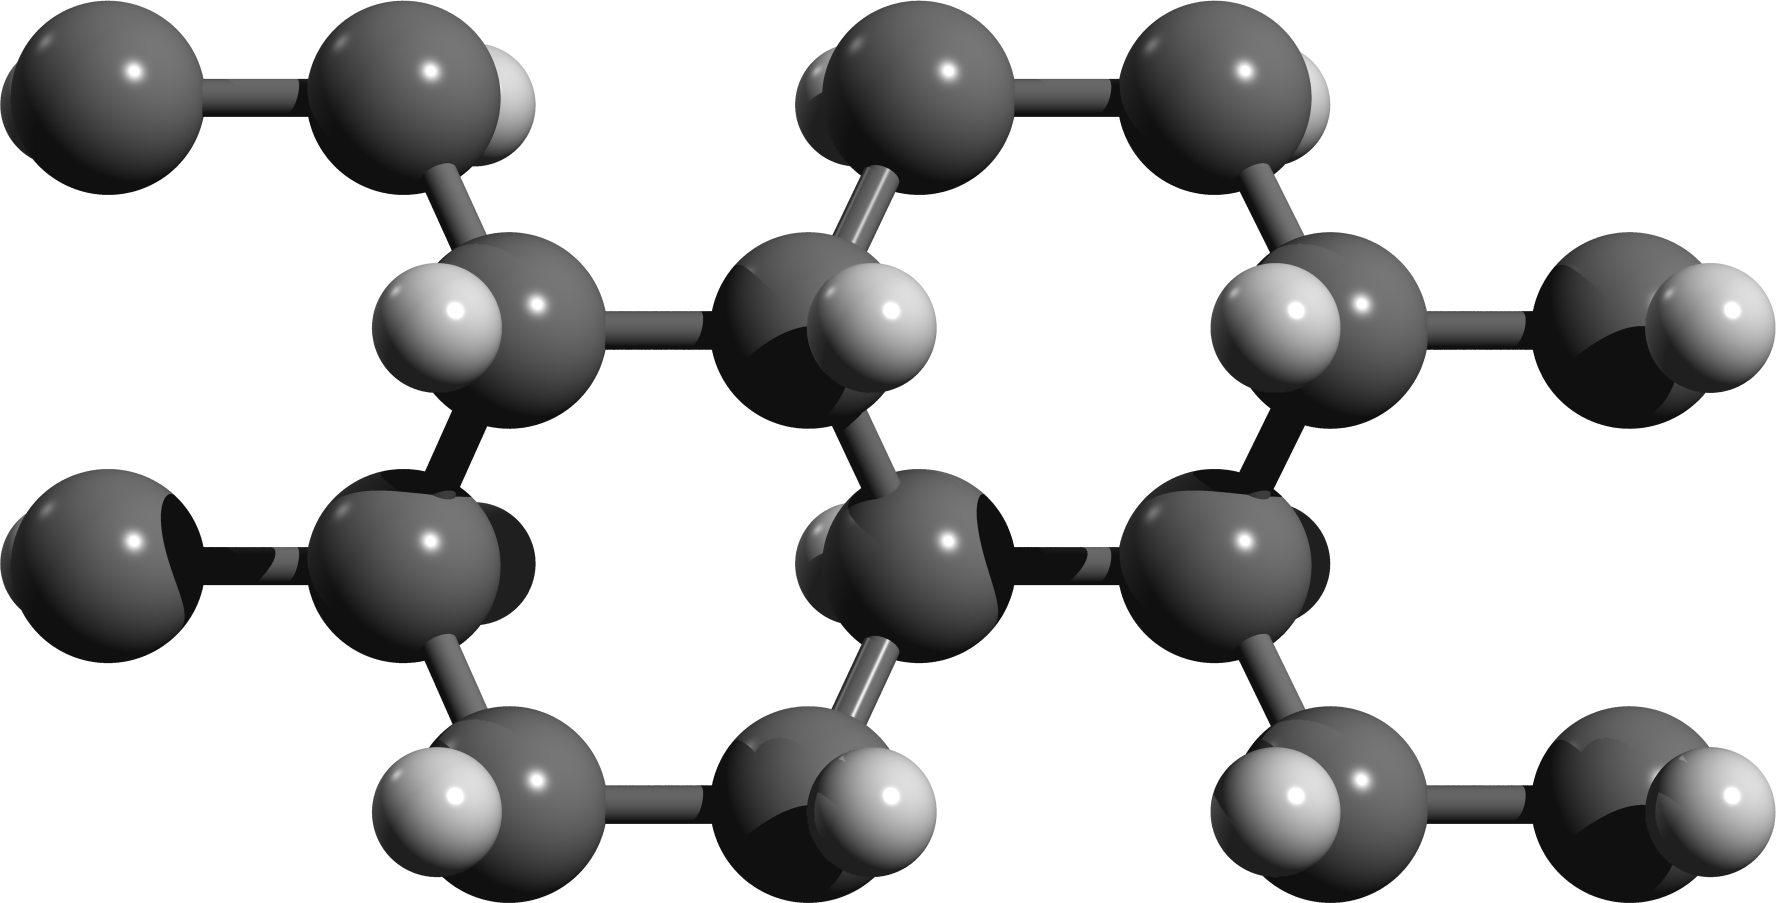
\includegraphics[width=0.8\textwidth]{figs/boat.png}\\
% % {\small 100\% of hydrogenation}

% \vspace{3mm}
% \end{center}

% \end{columns}

% \begin{center}

% {\huge Functionalization by hydrogenation}
% \end{center}
% \end{frame}

% %%%%%%%%%%%%%%%%%%%%%%%%%%%%%%%%%%%%%%%%%%%%%%%%%%%%%%%%%%%%%%%%%%%%%%%%%%%%%


% \begin{frame}

% \begin{columns}

% \column{0.5\textwidth}

% \centering
% \vspace{2mm}
% 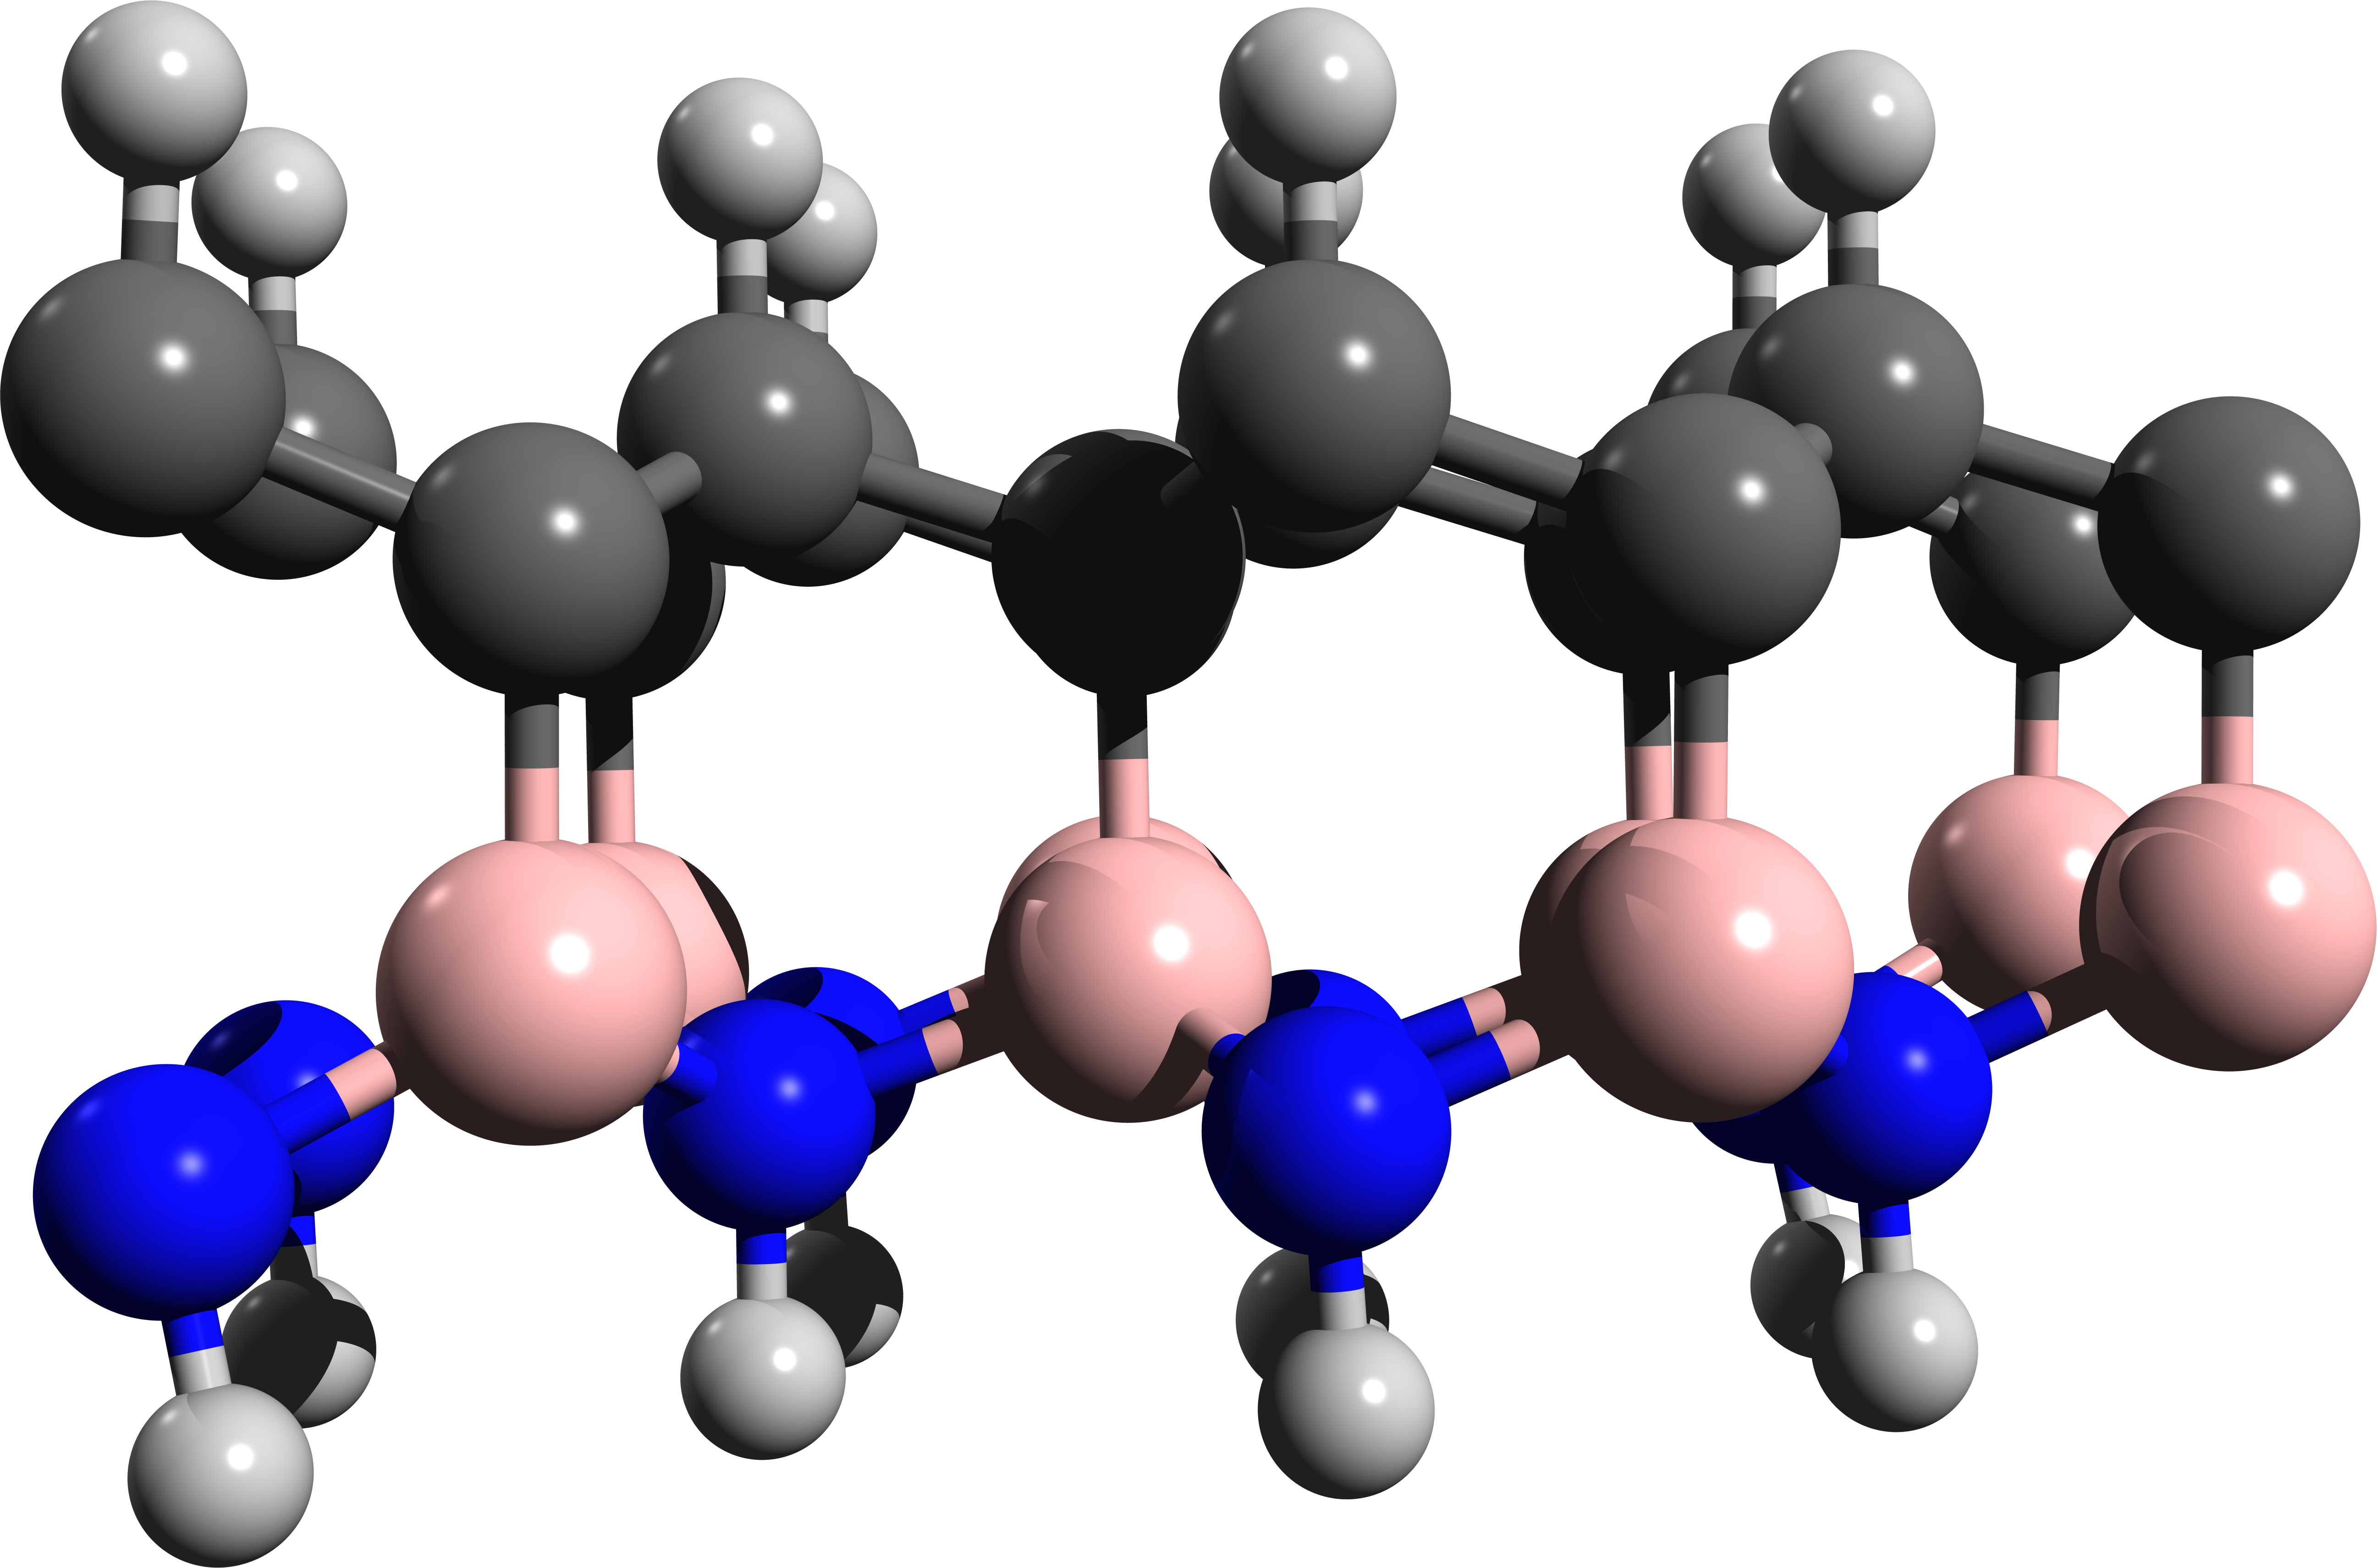
\includegraphics[width=0.75\textwidth]{figs/hnbGh-aa-1.png}
% \\ \vspace{4mm}
% 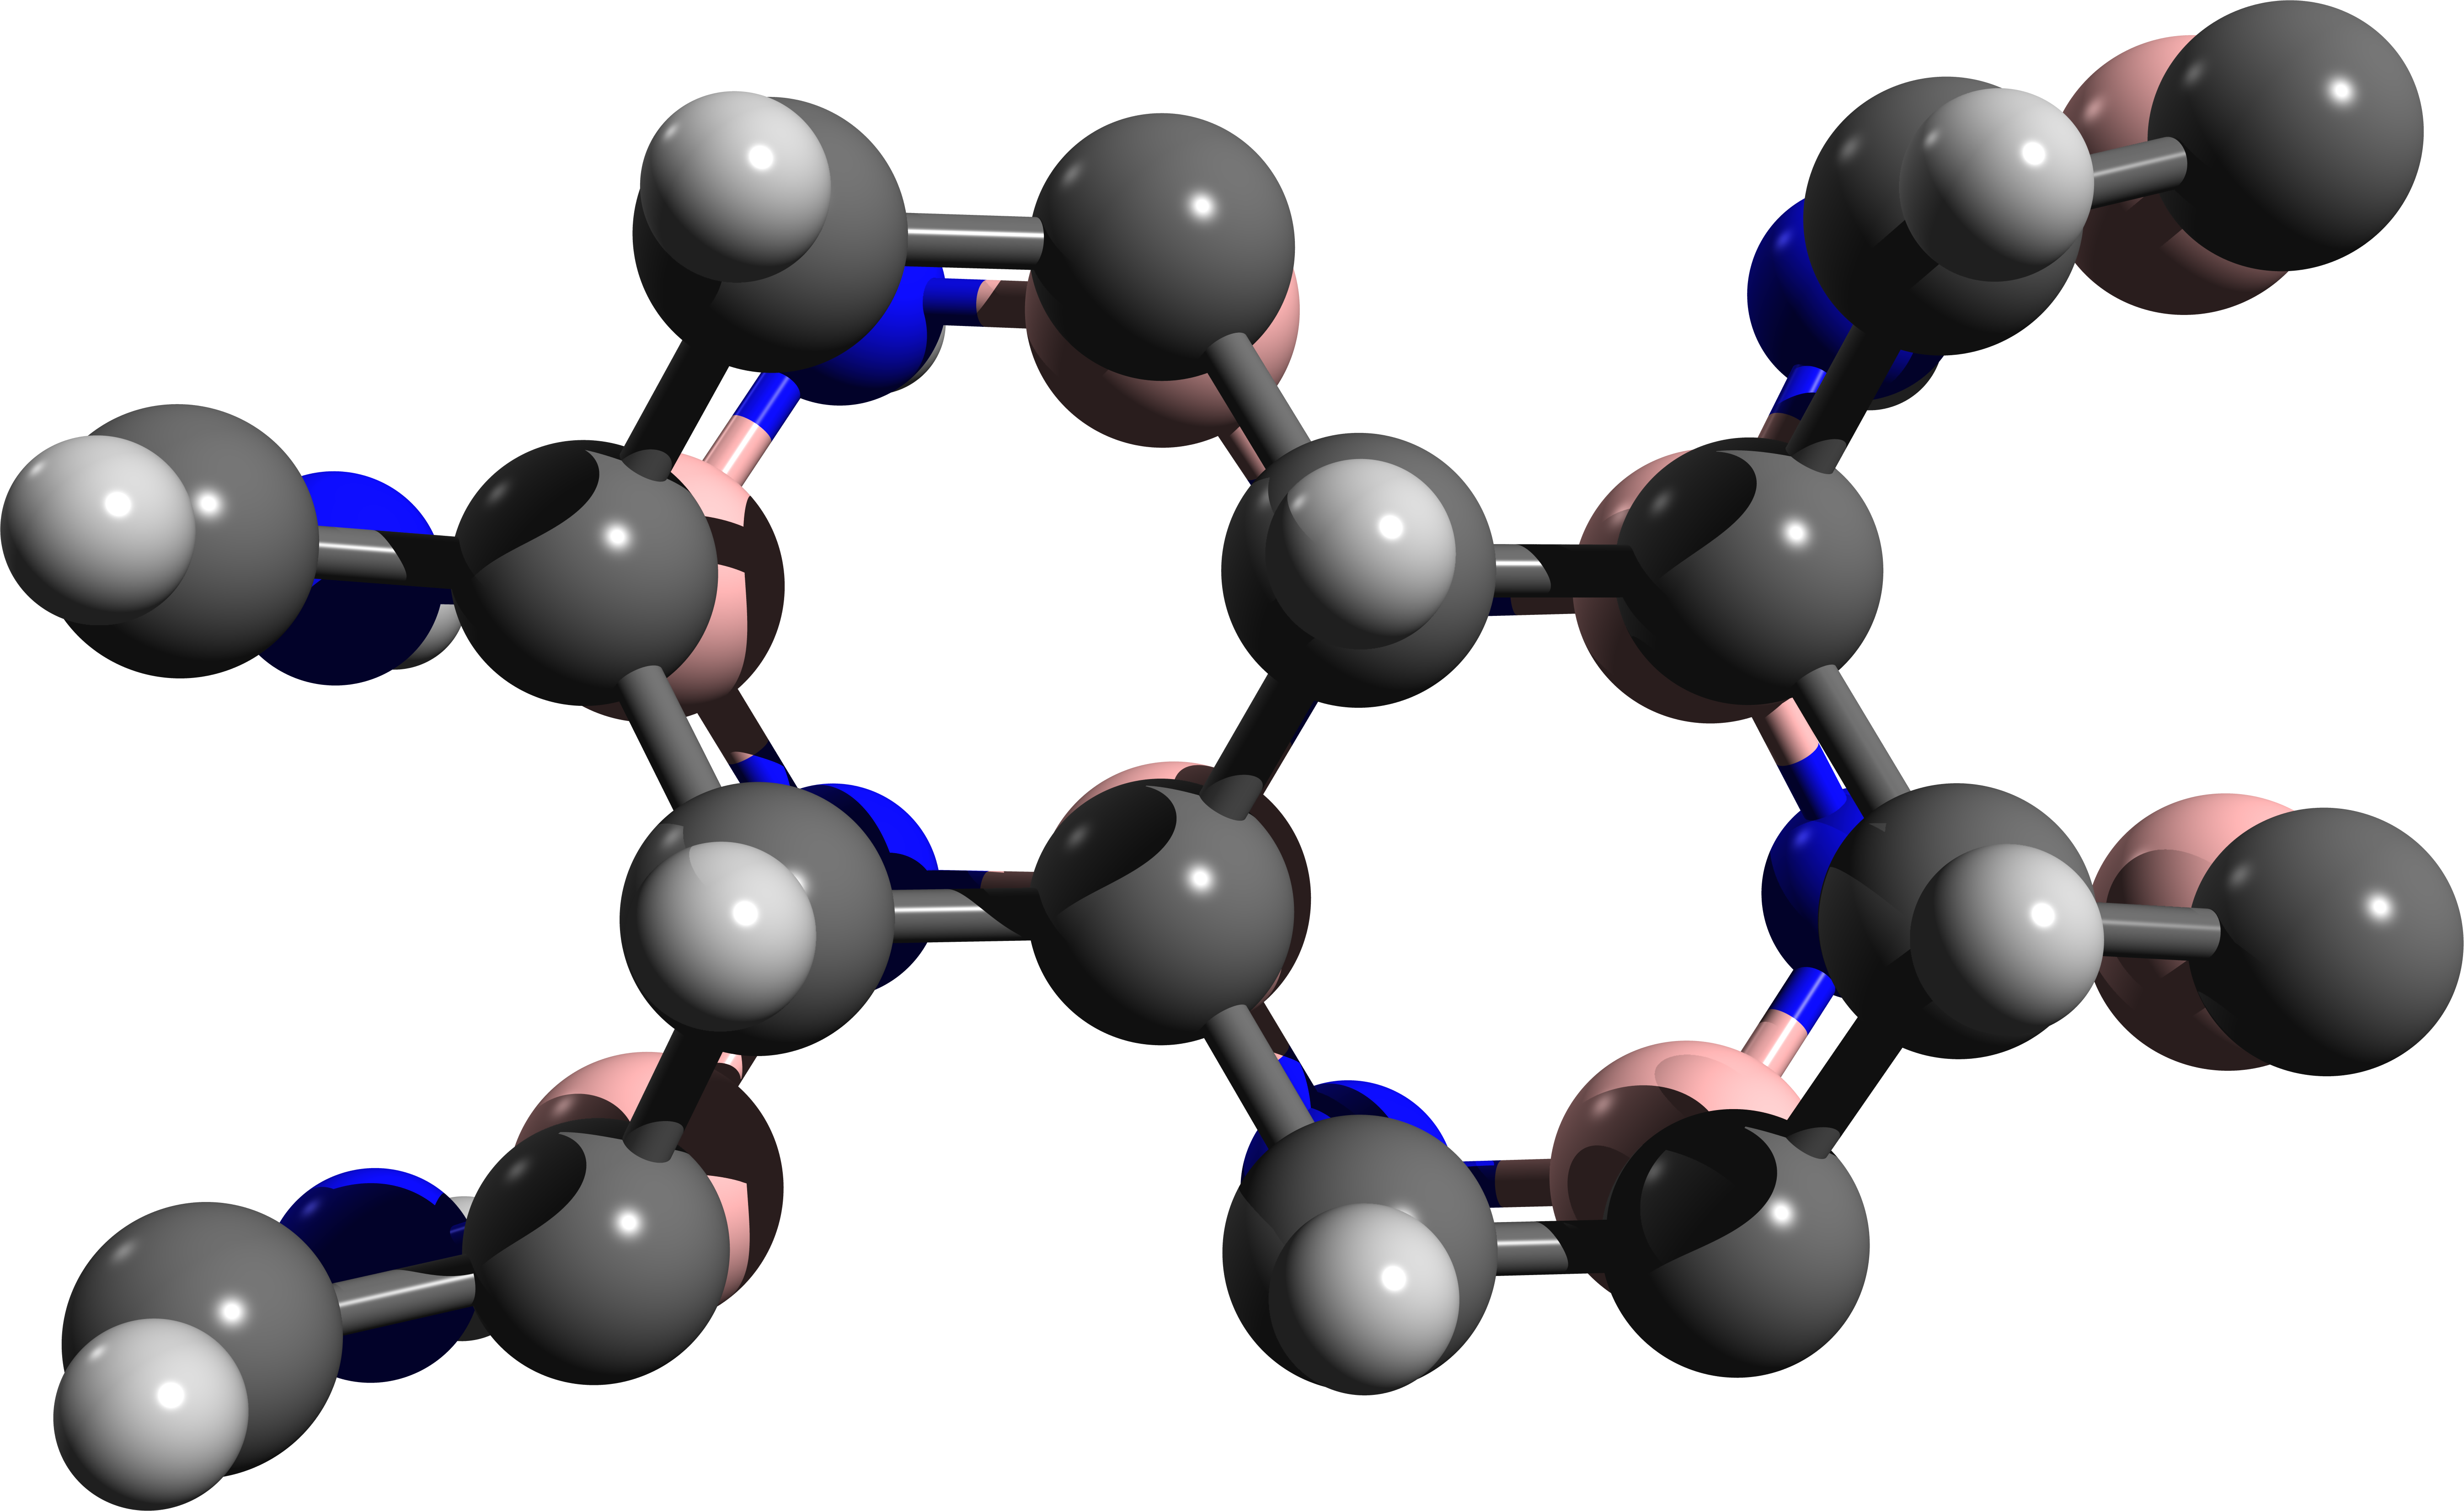
\includegraphics[width=0.75\textwidth]{figs/hnbGh-aa-2.png}

% \vspace{5mm}

% \column{0.5\textwidth}

% \centering
% \vspace{2mm}
% 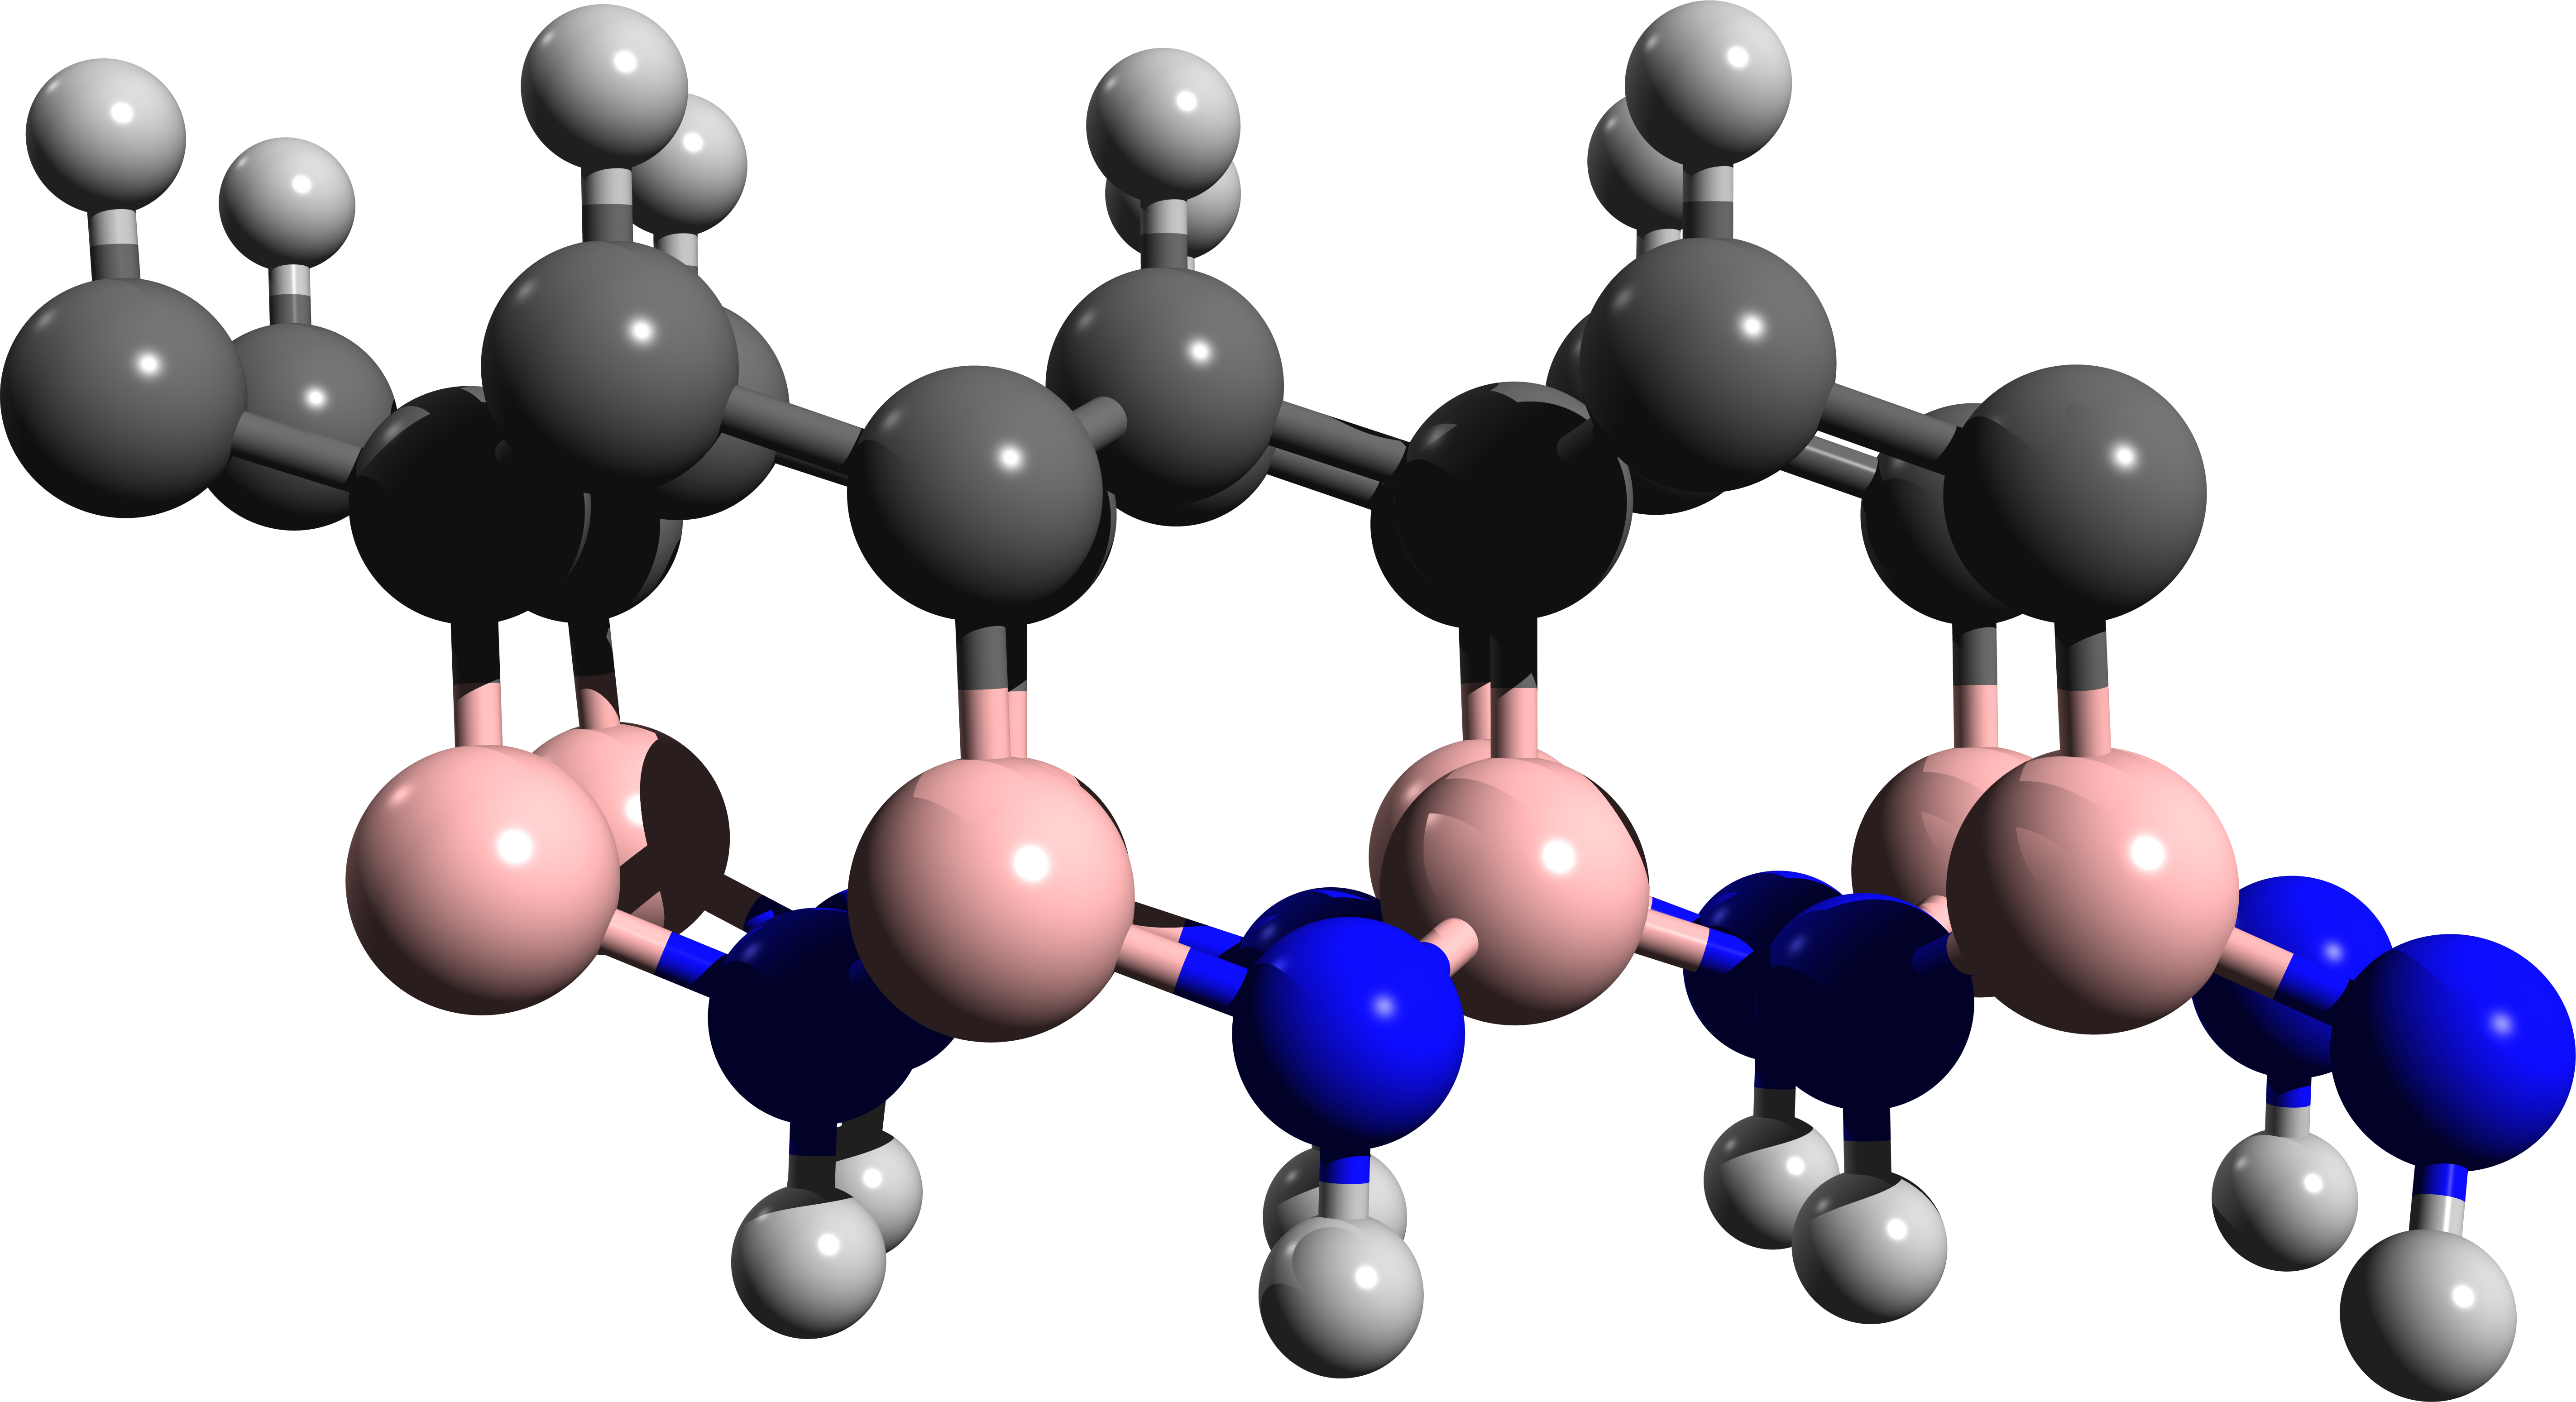
\includegraphics[width=0.75\textwidth]{figs/hnbGh-ab-1.png}
% \\ \vspace{4mm}
% 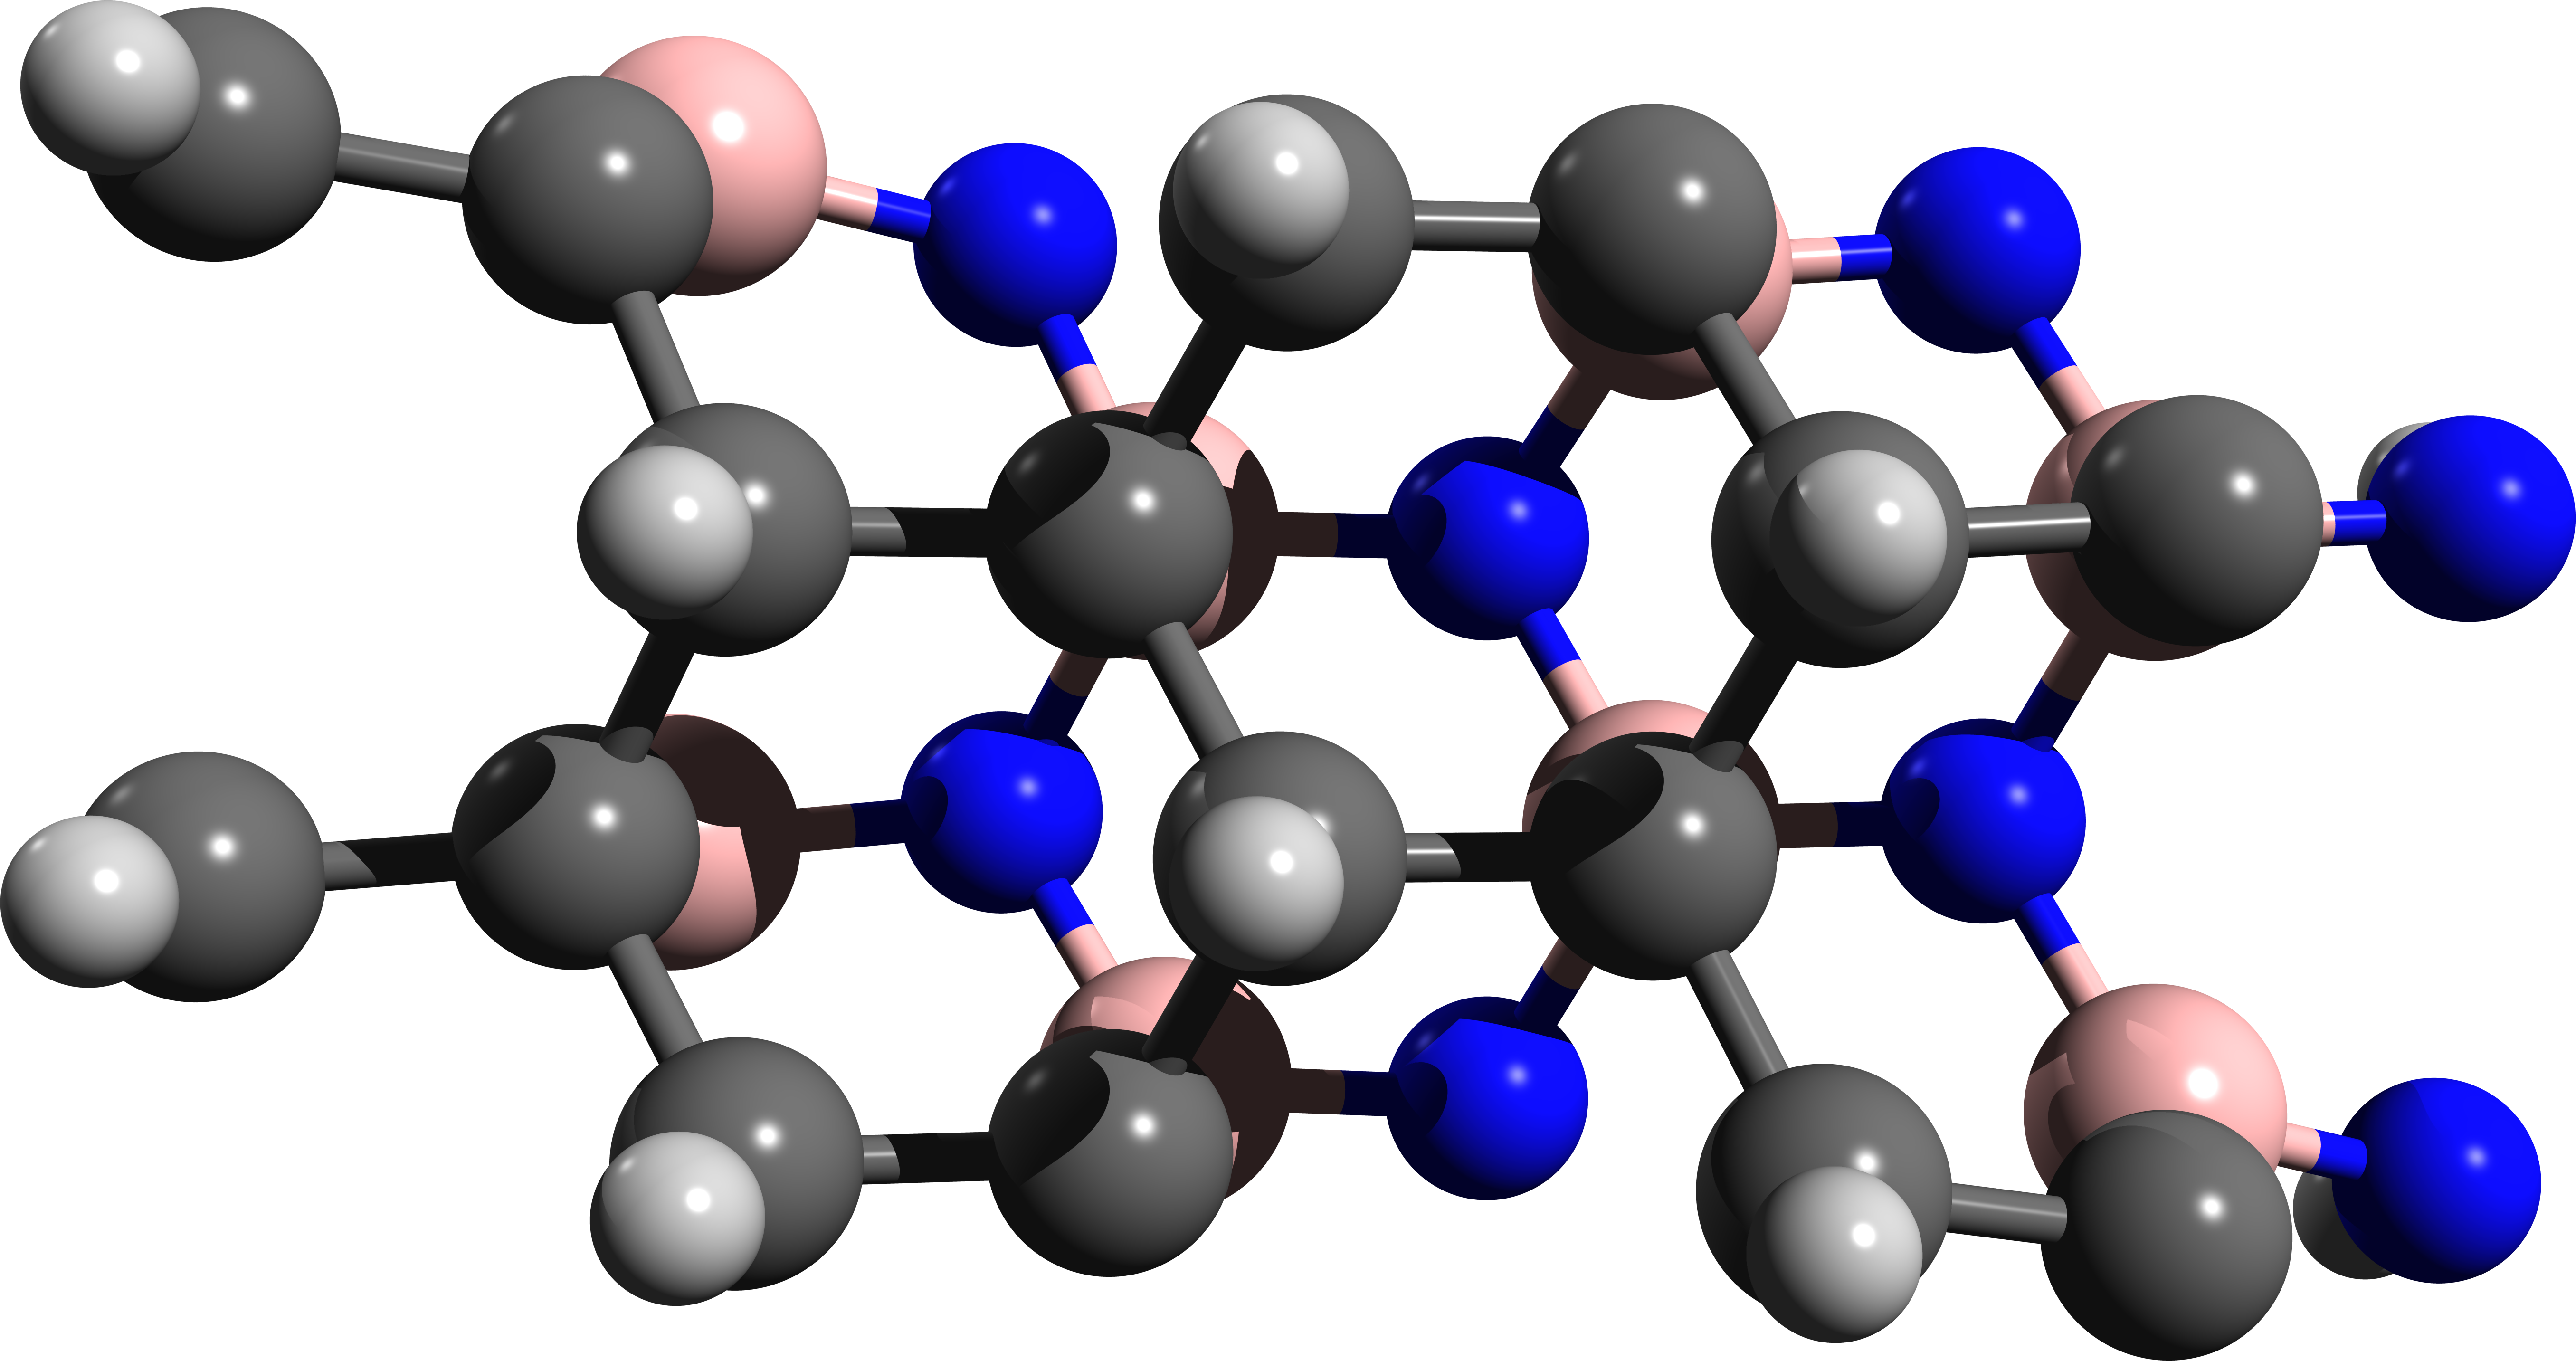
\includegraphics[width=0.75\textwidth]{figs/hnbGh-ab-2.png}

% \vspace{5mm}

% \end{columns}

% \begin{center}

% {\huge Hydrogen-boron-nitride-graphene functionalization}

% \end{center}
% \end{frame}

% %%%%%%%%%%%%%%%%%%%%%%%%%%%%%%%%%%%%%%%%%%%%%%%%%%%%%%%%%%%%%%%%%%%%%%%%%%%%%

% % %%%%%%%%%%%%%%%%%%%%%%%
% % \subsection{The Brillowin zone}
% % %%%%%%%%%%%%%%%%%%%%%%%

% % \begin{frame}

% % \vspace{-0.7cm}

% % \noindent\makebox[\linewidth]{\rule{\linewidth}{0.4pt}}

% % \vspace{-2.0mm}
% % \begin{center}
% % {\huge The Brillouin zone}
% % \end{center}

% % \vspace{-6mm}
% % \noindent\makebox[\linewidth]{\rule{\linewidth}{0.4pt}}

% % \begin{columns}
% % \column{0.5\textwidth}

% % \vspace{6.5mm}
% % \begin{figure}
% % \centering
% % 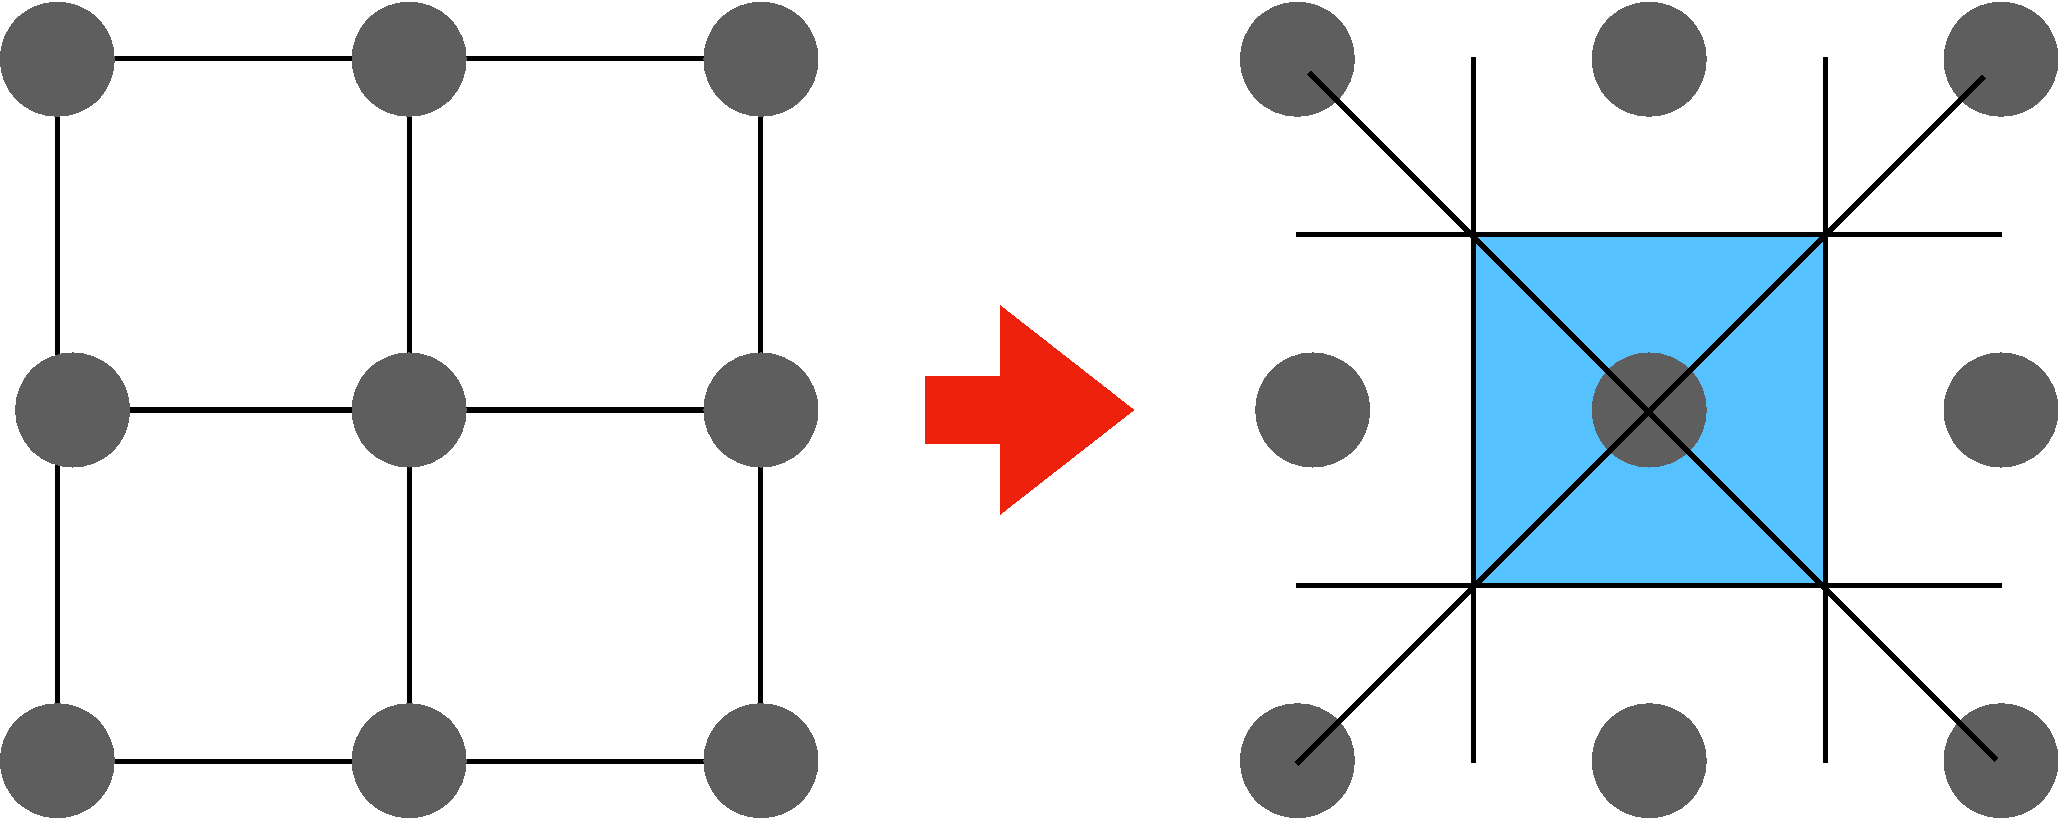
\includegraphics[width=0.9\textwidth]{figs/brill-sqr.pdf}
% % \end{figure}

% % \vspace{1mm}
% % \begin{center}
% % Square lattice.
% % \end{center}

% % \column{0.5\textwidth}

% % \begin{figure}
% % \centering
% % 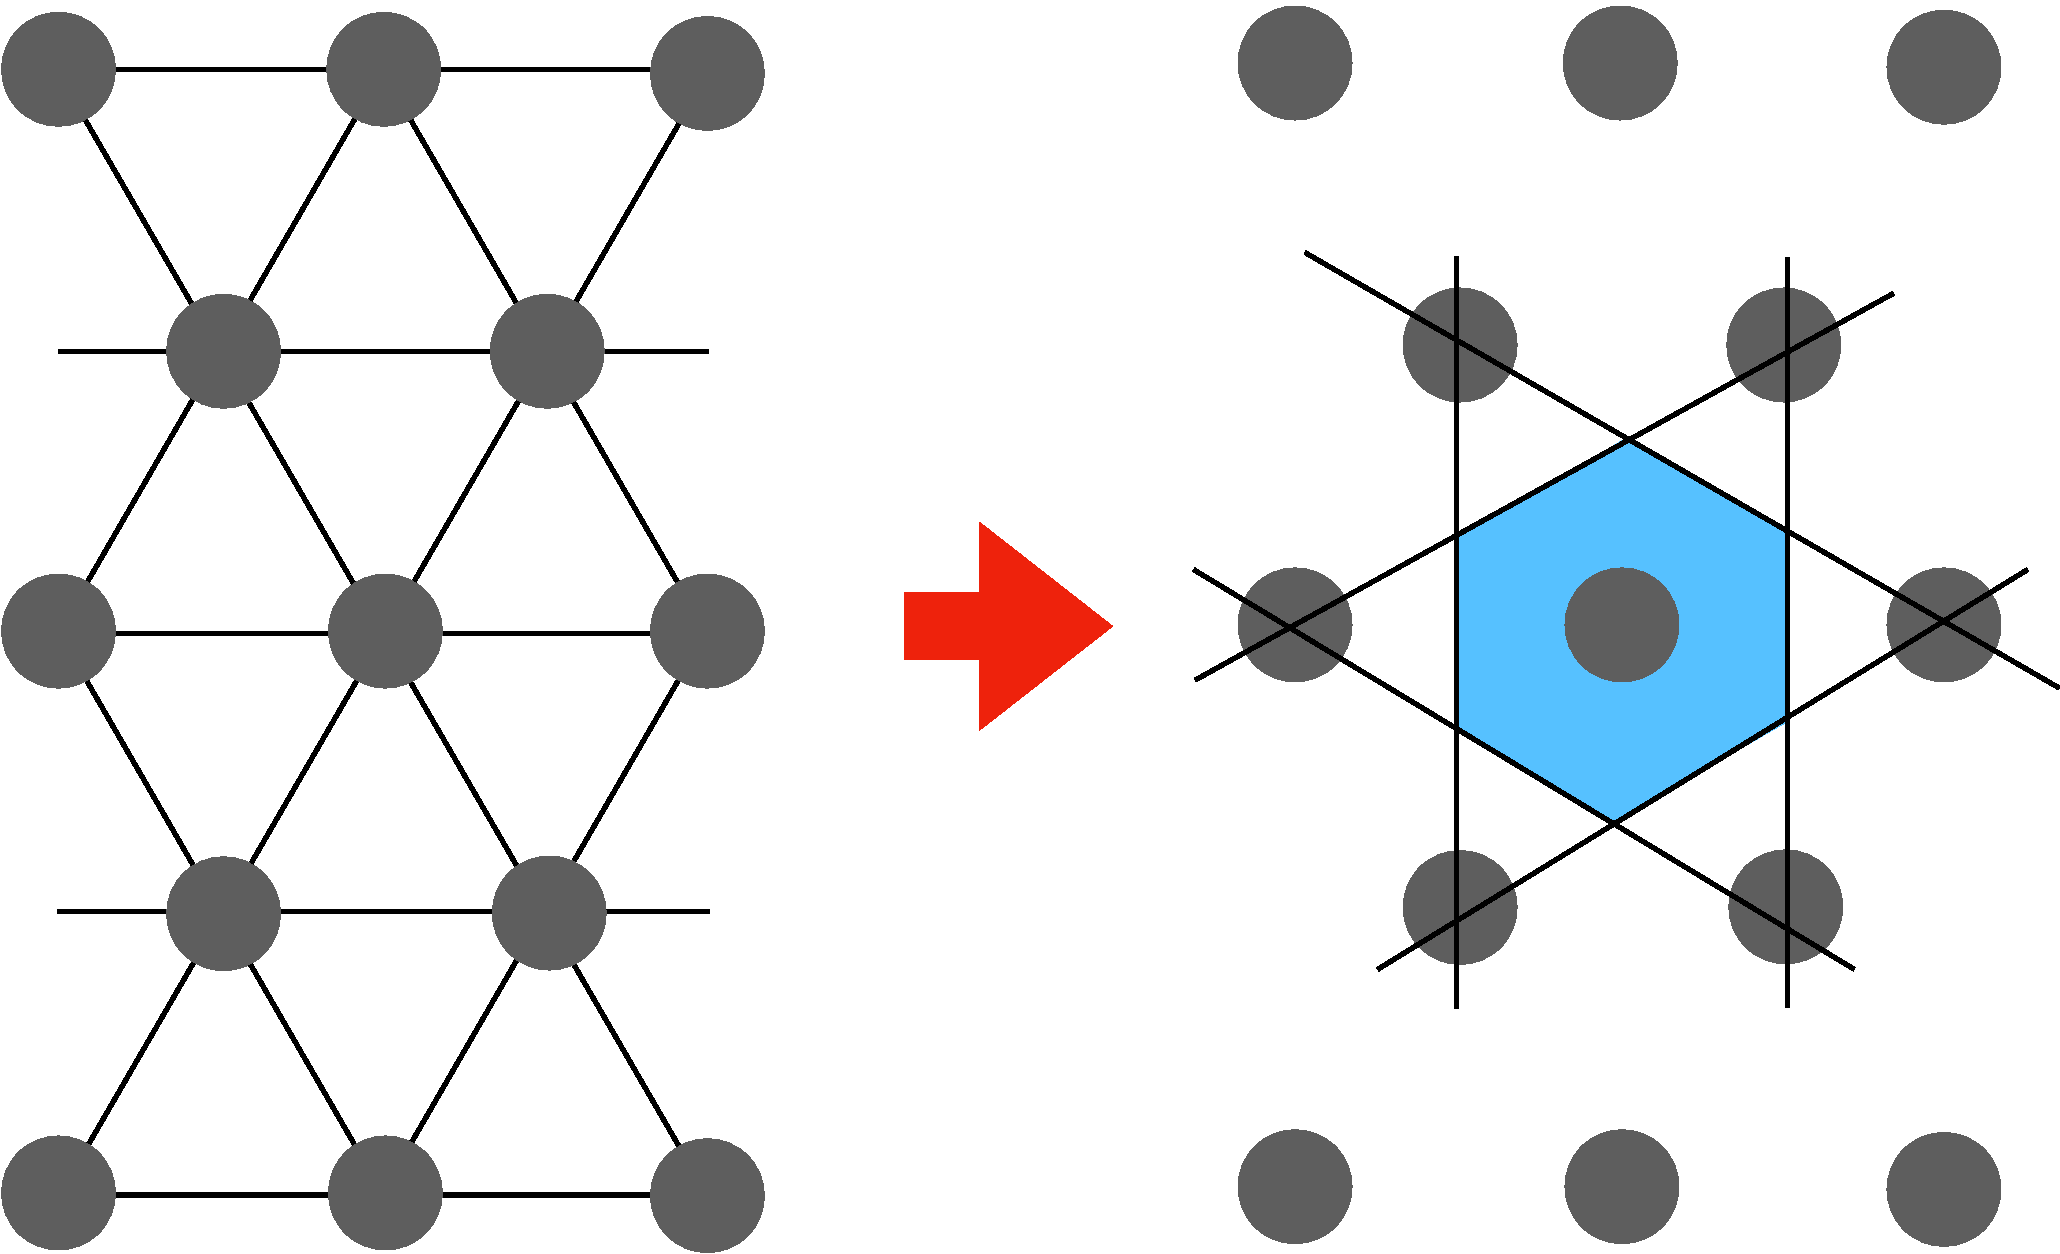
\includegraphics[width=0.9\textwidth]{figs/brill-hex.pdf}
% % \end{figure}

% % \begin{center}
% % Hexagonal lattice.
% % \end{center}

% % \end{columns}

% % \begin{center}
% % The boundaries of this cell are given by planes related 
% % to points on the reciprocal lattice.
% % \end{center}

% % \end{frame}



%%%%%%%%%%%%%%%%%%%%%%%%%%%%%%%%%%%%%%%%%%%%%%%%%%%%%%%%%%%%%%%%%%%%%%%%%%%%%
\section{The structures}
%%%%%%%%%%%%%%%%%%%%%%%%%%%%%%%%%%%%%%%%%%%%%%%%%%%%%%%%%%%%%%%%%%%%%%%%%%%%%


%%%%%%%%%%%%%%%%%%%%%%%
\subsection{Centrosymmetric Materials}
%%%%%%%%%%%%%%%%%%%%%%%

\begin{frame}

\vspace{-0.2cm}

\noindent\makebox[\linewidth]{\rule{\linewidth}{0.4pt}}

\vspace{-2.0mm}
\begin{center}
{\large Centrosymmetric Materials}
\end{center}

\vspace{-5mm}
\noindent\makebox[\linewidth]{\rule{\linewidth}{0.4pt}}

\begin{center}
A centrosymmetric system presents inversion of symmetry, such
that a point $p(a, b, c)$ corresponds a point $p'(-a, -b, -c)$.
\end{center}


\begin{figure}[h!]
\begin{tikzpicture}

\node[anchor=south west,inner sep=0] at (0.2,-0.3) 
{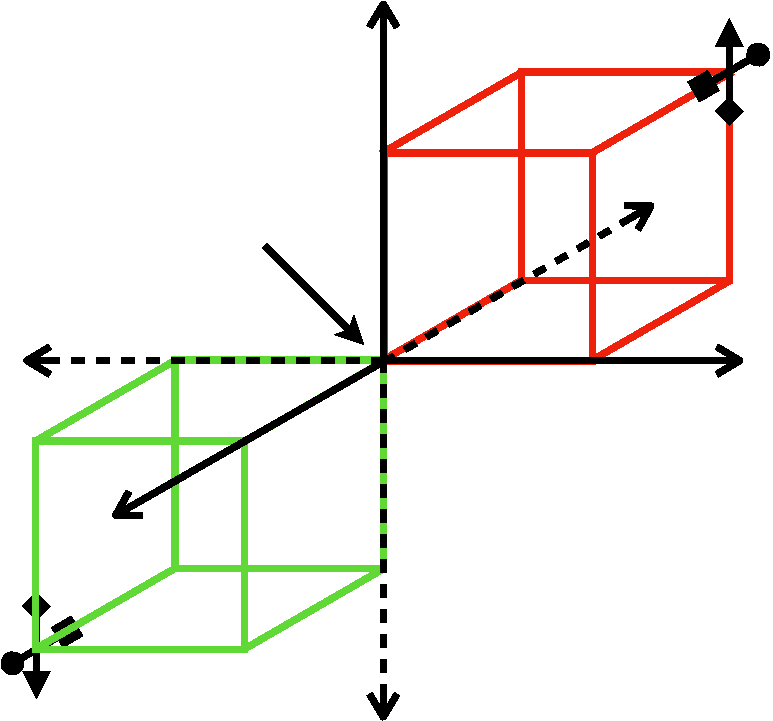
\includegraphics[width=0.5\textwidth]{figs/inversion.pdf}};
\draw [] (5.40, 2.20) node [right] {$x$};
\draw [] (2.65, 5.00) node [right] {$y$};
\draw [] (0.50, 1.00) node [right] {$z$};
\draw [] (5.40, 4.80) node [right] {$p(a,b,c)$};
\draw [](-2.20, 0.00) node [right] {$p'(-a,-b,-c)$};
\draw [](-0.60, 3.20) node [right] {\rmfamily inversion point};

\end{tikzpicture}
\end{figure}


\end{frame}

%%%%%%%%%%%%%%%%%%%%%%%%%%%%%%%%%%%%%%%%%%%%%%%%%%%%%%%%%%%%%%%%%%%%%%%%%%%%%




%%%%%%%%%%%%%%%%%%%%%%%
\subsection{Alt structure}
%%%%%%%%%%%%%%%%%%%%%%%


\begin{frame}

\vspace{-3mm}
\begin{columns}

\column{0.7\textwidth}
\flushright
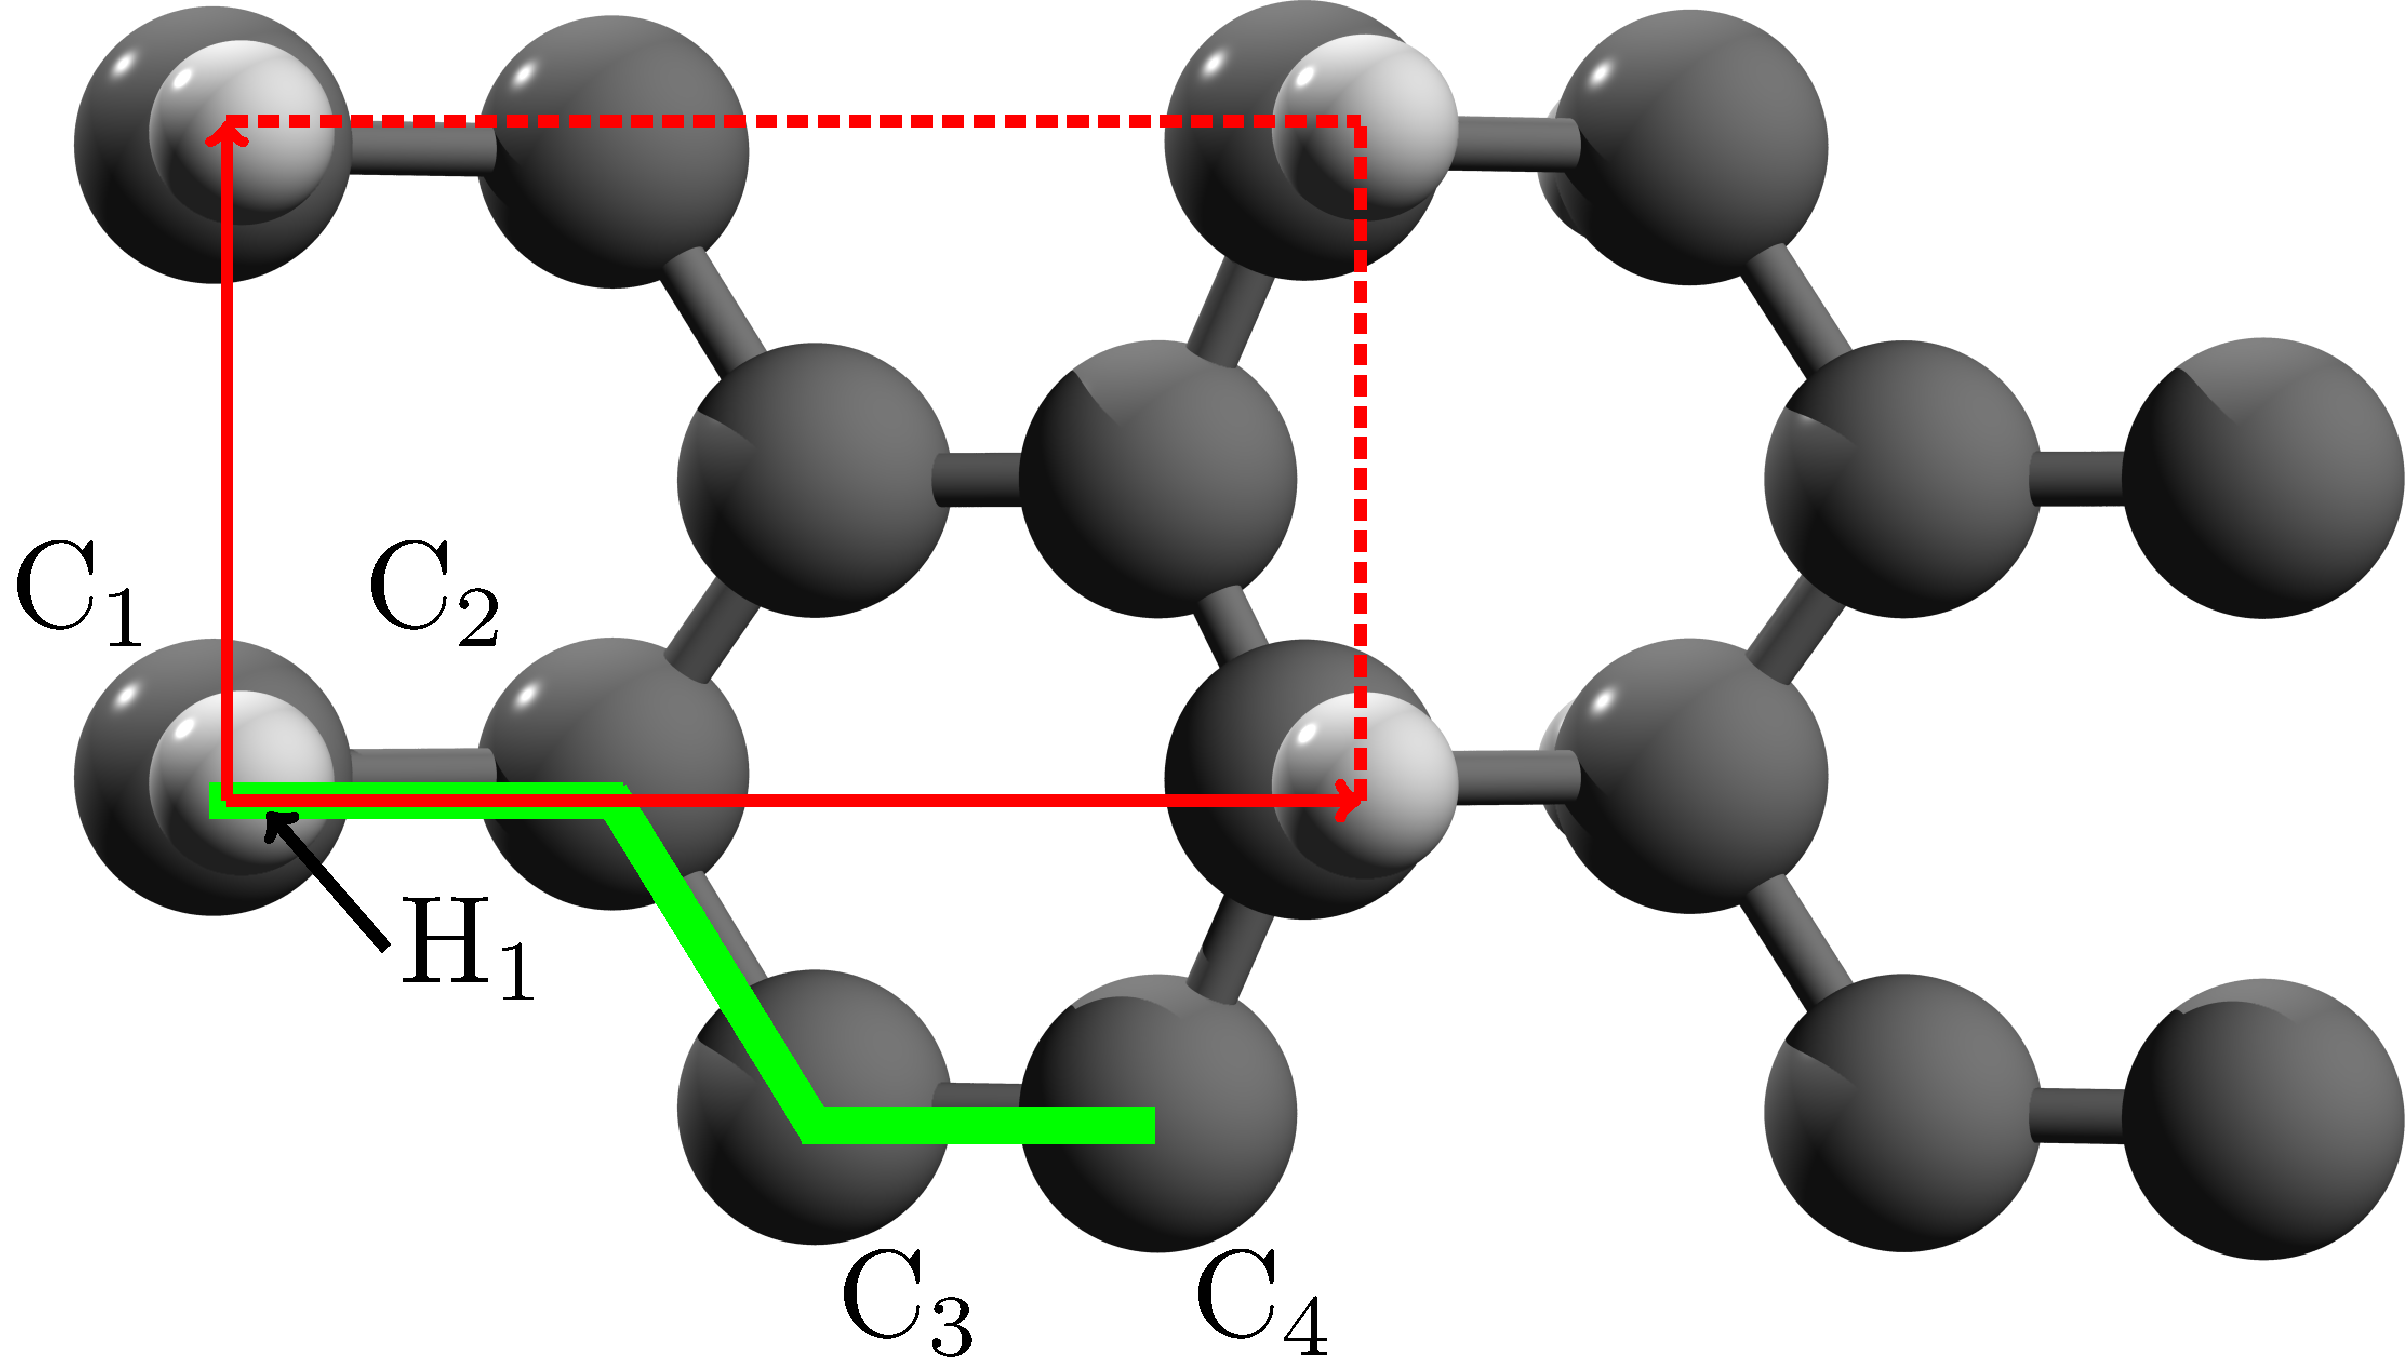
\includegraphics[width=0.9\textwidth]{figs/alt1.pdf}

\vspace{5mm}

\column{0.3\textwidth}
\flushleft
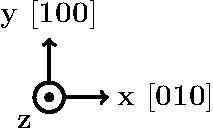
\includegraphics[width=0.9\textwidth]{figs/arrows1.pdf}

\end{columns}

\vspace{-5mm}

\begin{columns}

\column{0.7\textwidth}
\flushright
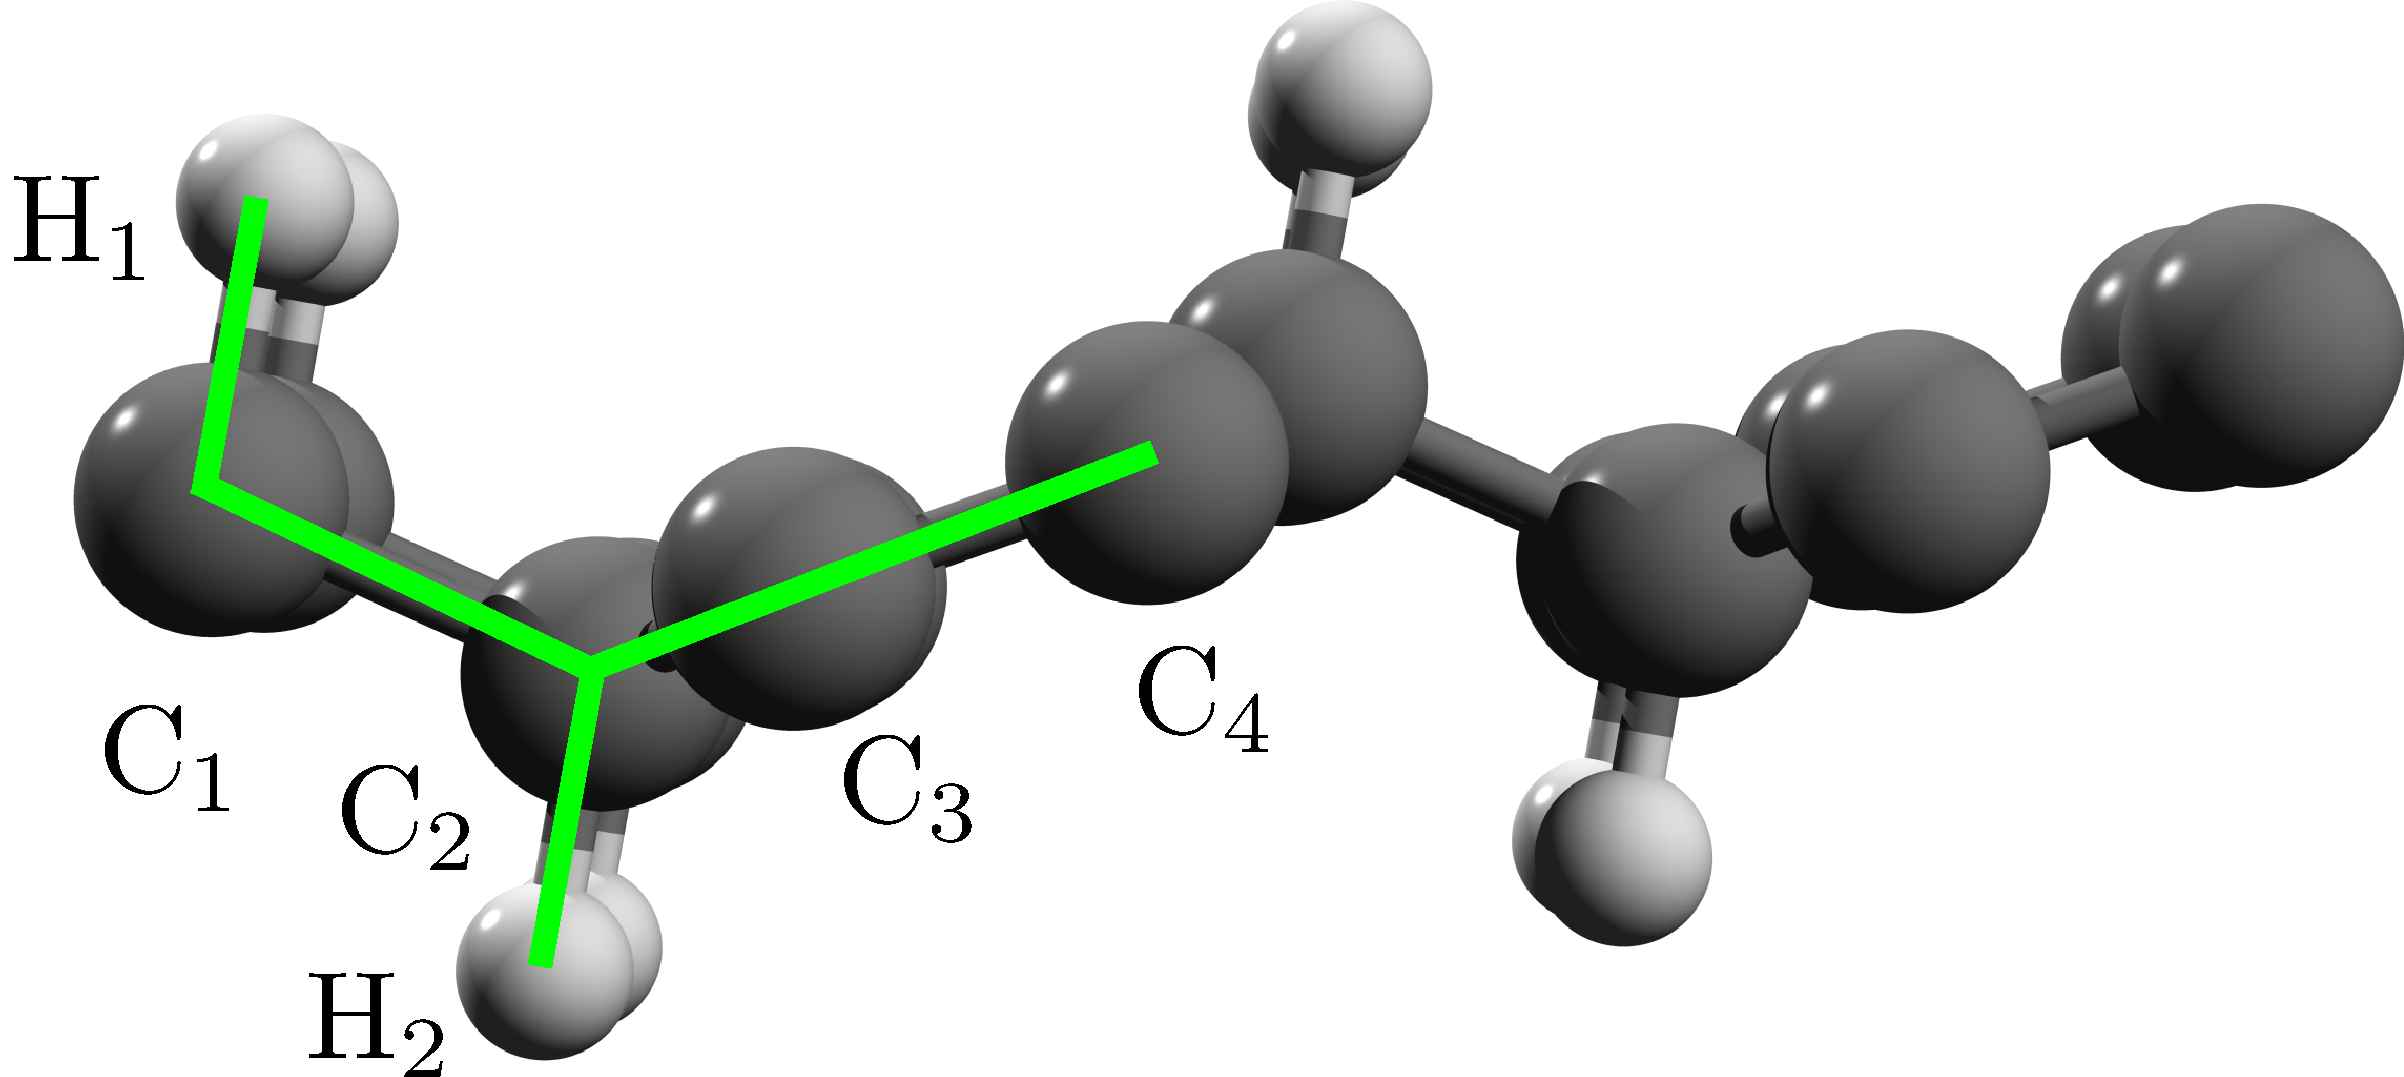
\includegraphics[width=0.9\textwidth]{figs/alt2.pdf}

\vspace{5mm}

\column{0.3\textwidth}
\flushleft
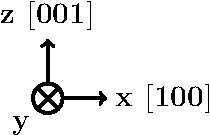
\includegraphics[width=0.9\textwidth]{figs/arrows2.pdf}

\end{columns}

\vspace{-4mm}
\begin{center}
{\Large Alt structure:} 50\% hydrogenation; hydrogen at bot sides.
\end{center}

\end{frame}

%%%%%%%%%%%%%%%%%%%%%%%%%%%%%%%%%%%%%%%%%%%%%%%%%%%%%%%%%%%%%%%%%%%%%%%%%%%%%


%%%%%%%%%%%%%%%%%%%%%%%
\subsection{Up structure}
%%%%%%%%%%%%%%%%%%%%%%%


\begin{frame}

\vspace{-3mm}
\begin{columns}

\column{0.7\textwidth}
\flushright
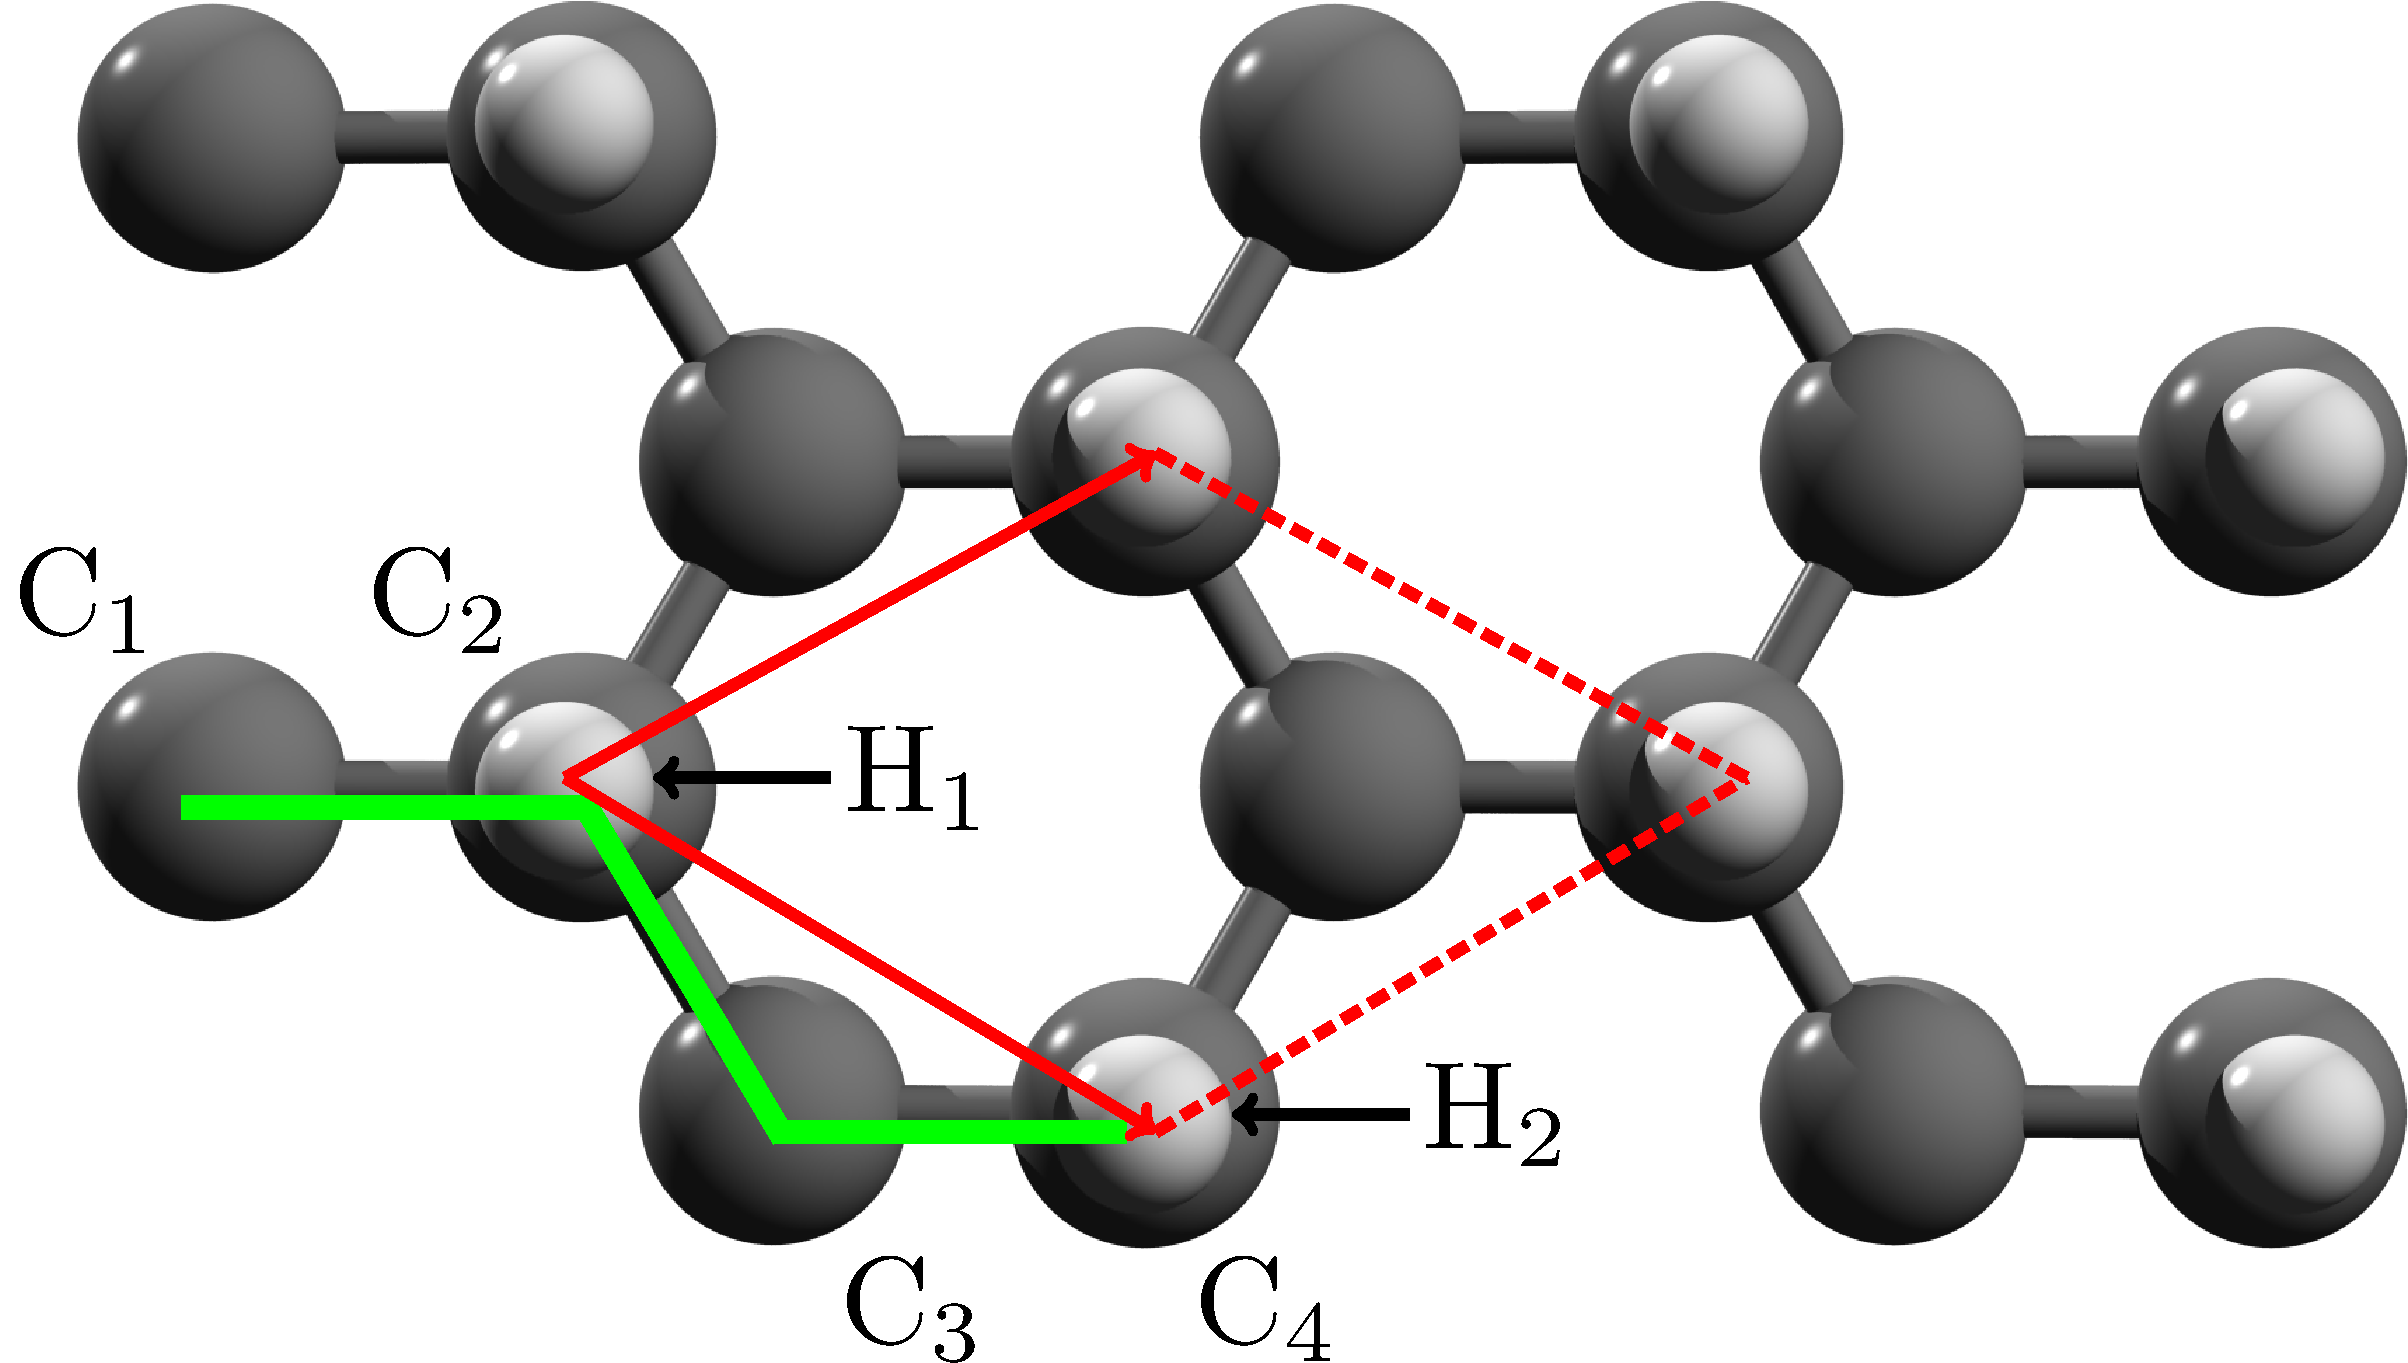
\includegraphics[width=0.9\textwidth]{figs/up1.pdf}

\vspace{5mm}

\column{0.3\textwidth}
\flushleft
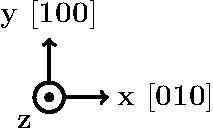
\includegraphics[width=0.9\textwidth]{figs/arrows1.pdf}

\end{columns}

\vspace{-5mm}

\begin{columns}

\column{0.7\textwidth}
\flushright
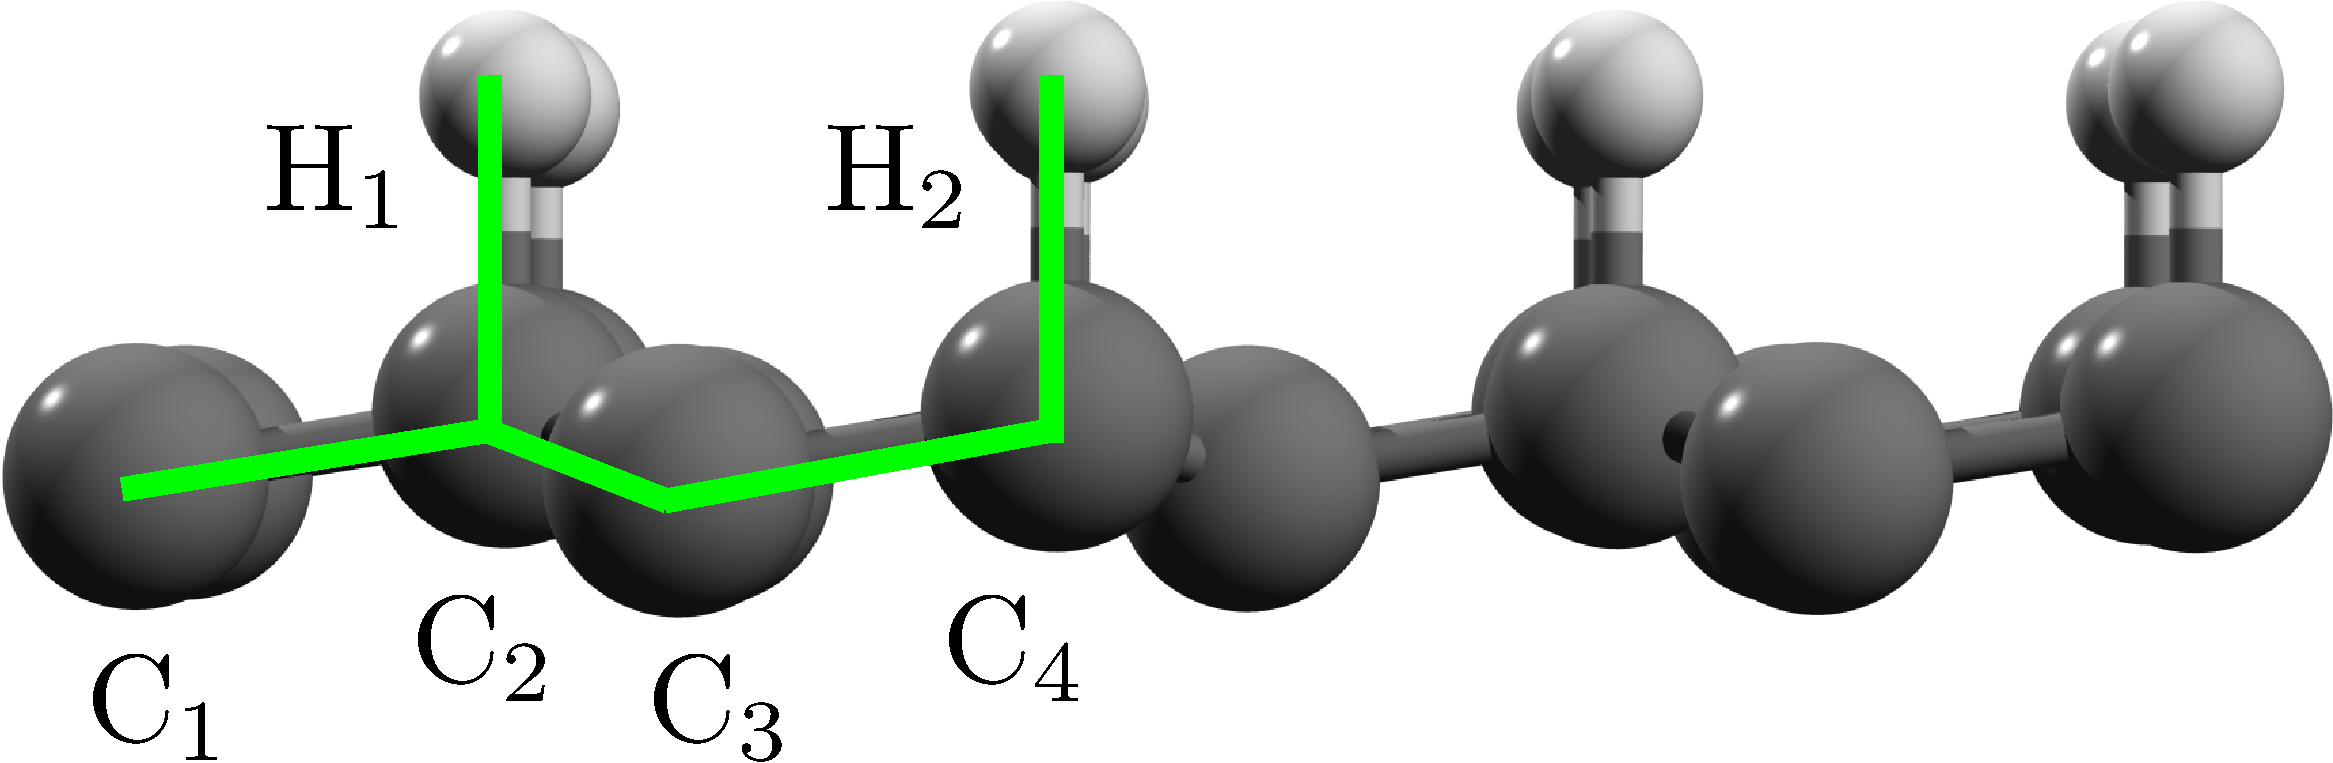
\includegraphics[width=0.9\textwidth]{figs/up2.pdf}

\vspace{5mm}

\column{0.3\textwidth}
\flushleft
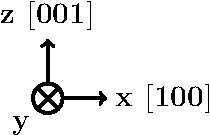
\includegraphics[width=0.9\textwidth]{figs/arrows2.pdf}

\end{columns}

\vspace{-4mm}
\begin{center}
{\Large Up structure:} 50\% hydrogenation; hydrogen on the upper side.
\end{center}

\end{frame}


%%%%%%%%%%%%%%%%%%%%%%%%%%%%%%%%%%%%%%%%%%%%%%%%%%%%%%%%%%%%%%%%%%%%%%%%%%%%%





%%%%%%%%%%%%%%%%%%%%%%%%%%%%%%%%%%%%%%%%%%%%%%%%%%%%%%%%%%%%%%%%%%%%%%%%%%%%%
\section{Theory} 
%%%%%%%%%%%%%%%%%%%%%%%%%%%%%%%%%%%%%%%%%%%%%%%%%%%%%%%%%%%%%%%%%%%%%%%%%%%%%



%%%%%%%%%%%%%%%%%%%%%%%
\subsection{Optical spin injection and DSP}
%%%%%%%%%%%%%%%%%%%%%%%



\begin{frame}

\vspace{-0.2cm}

\noindent\makebox[\linewidth]{\rule{\linewidth}{0.4pt}}

\vspace{-2.0mm}
\begin{center}
{\large Optical spin injection and degree of spin polarization (DSP)}
\end{center}

\vspace{-6mm}
\noindent\makebox[\linewidth]{\rule{\linewidth}{0.4pt}}


{\small

\begin{columns}
    
\column{0.5\textwidth}
\begin{itemize}

\item 
Spintronics is based in the injection, detection and transport of spin
polarized electrons in nonmagnetic materials.\footnote[frame]{\tiny A. Fert et.
al. Rev. Mod. Phys., 80(4):1517, 2008.}

\item 
Spin polarized electrons in a given $a$ direction can be injected through
circularly polarized light.\footnote[frame]{\tiny N. Arzate et al. Phys. Rev.
B, 90(20):205310, 2014.}

\end{itemize}


\column{0.5\textwidth}

\begin{figure}[h!]
\begin{tikzpicture}

\node[anchor=south west,inner sep=0] at (0.2,-0.3) 
{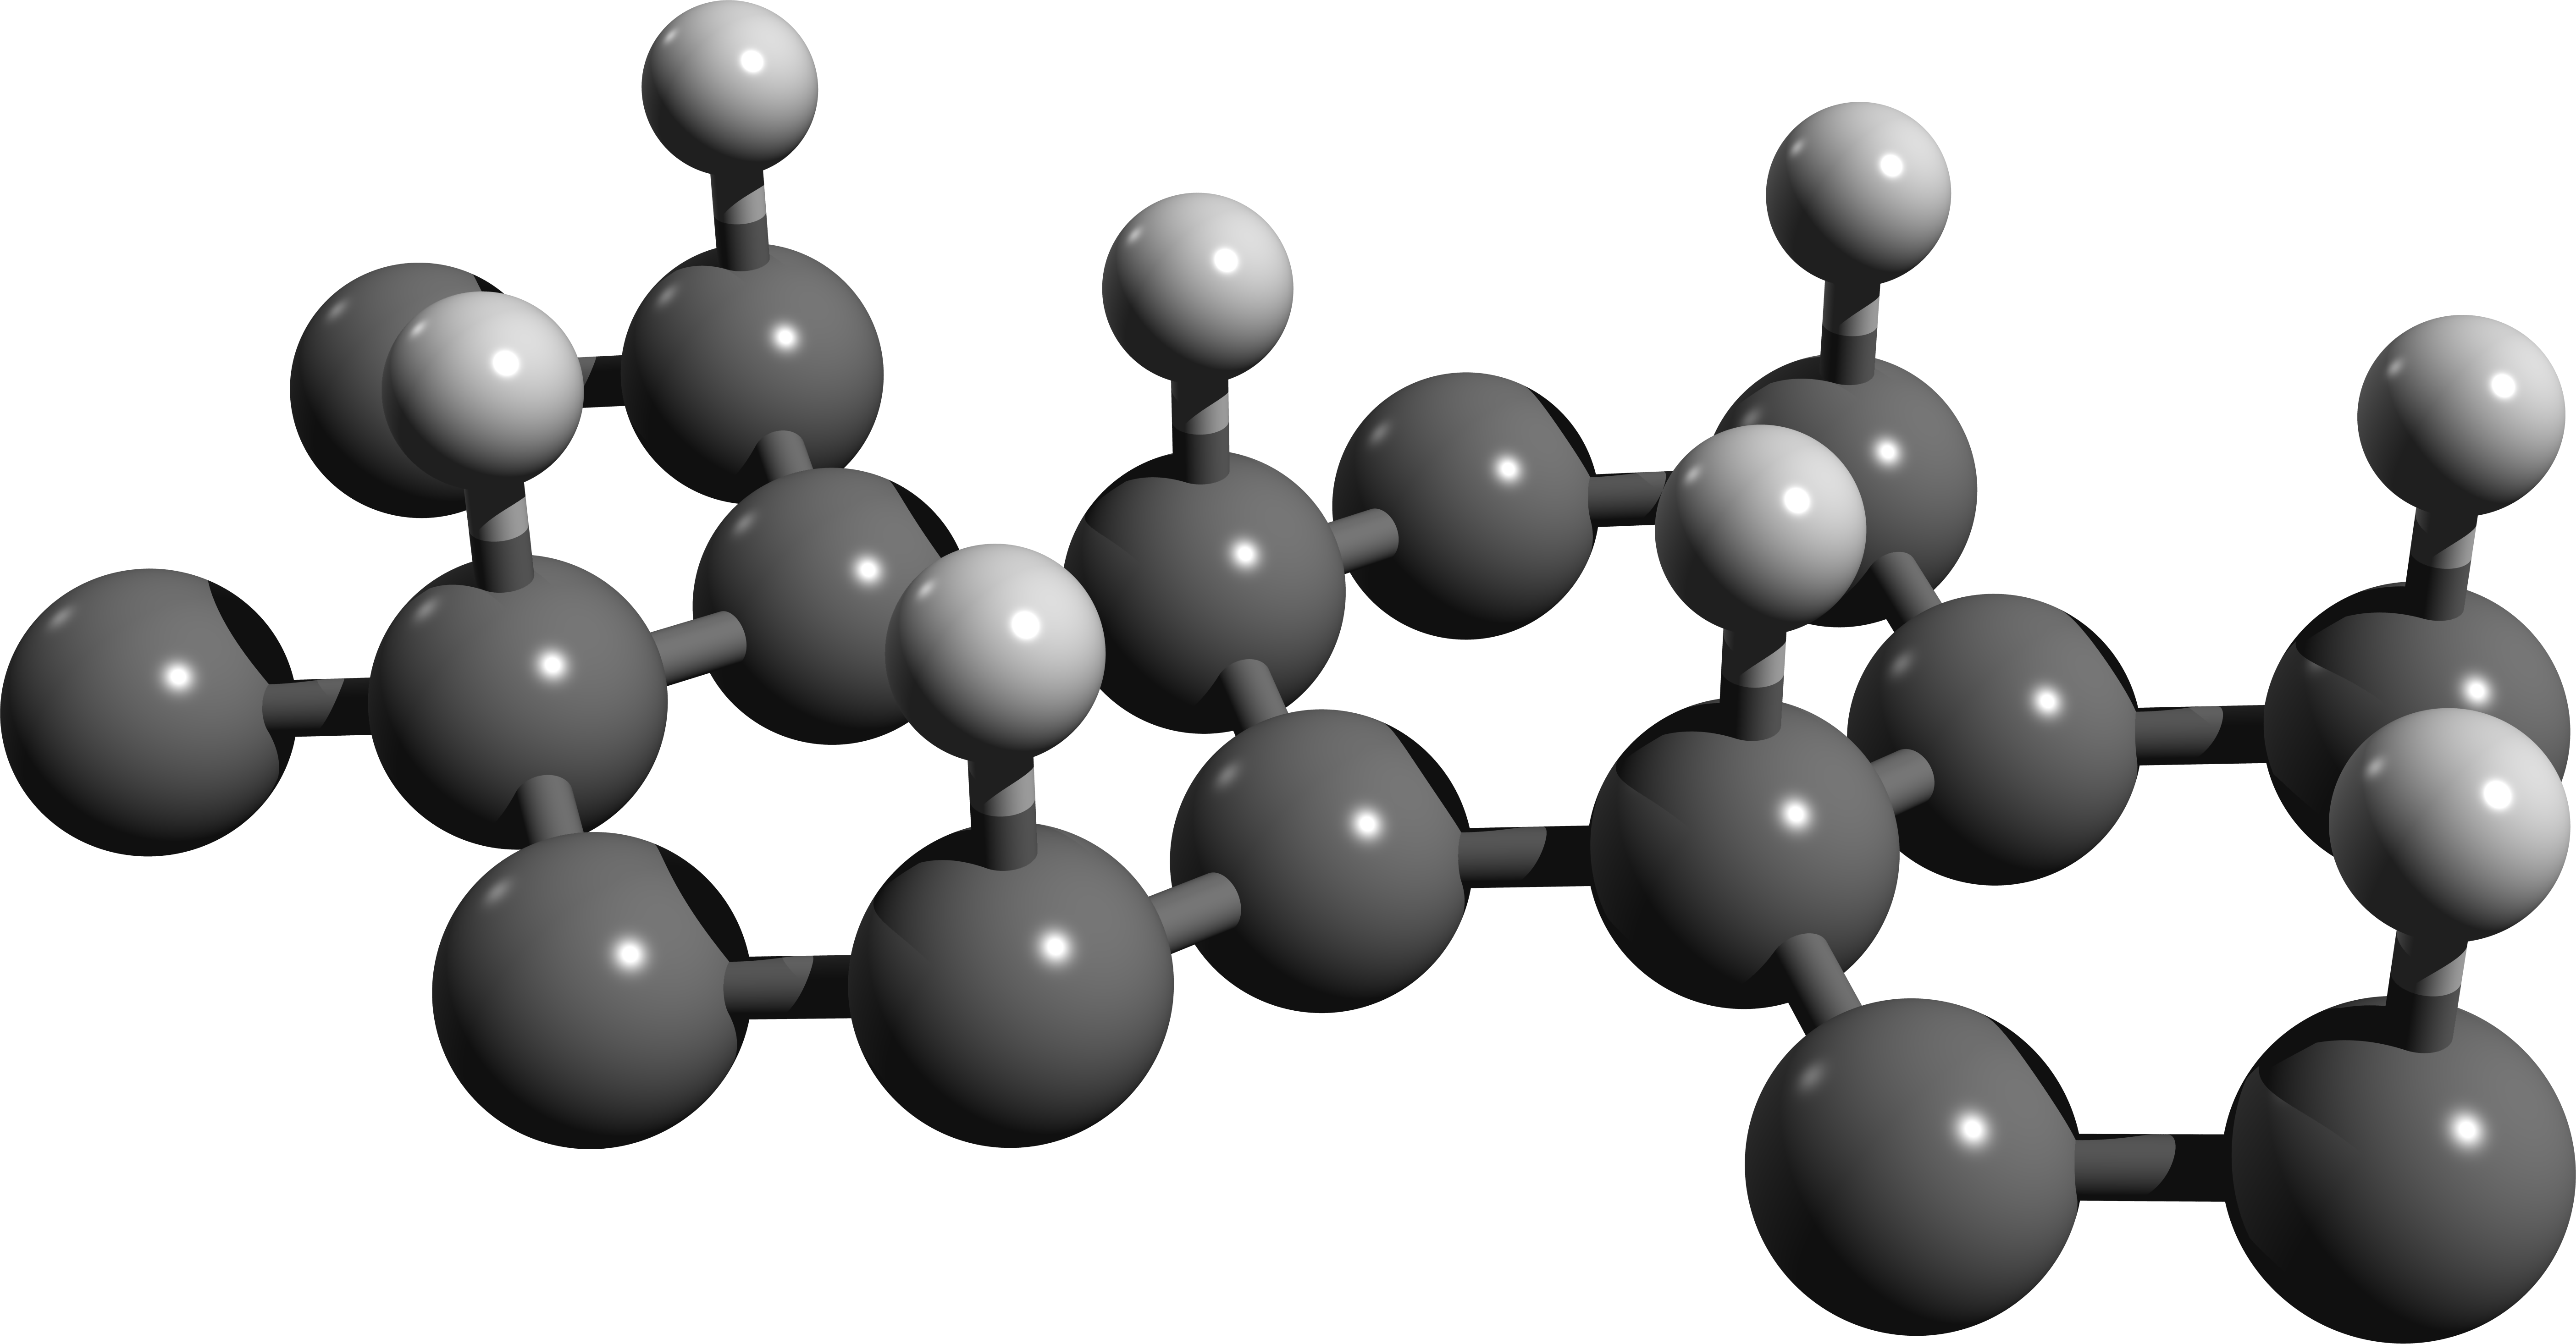
\includegraphics[width=1.0\textwidth]{figs/up3.png}};
\node[anchor=south west,inner sep=0] at (1.5,-1.2) 
{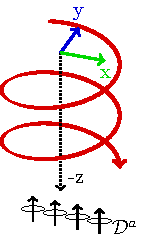
\includegraphics[width=0.6\textwidth]{figs/helix1.pdf}};

\end{tikzpicture}
\end{figure}


\end{columns}

}

\end{frame}

%%%%%%%%%%%%%%%%%%%%%%%%%%%%%%%%%%%%%%%%%%%%%%%%%%%%%%%%%%%%%%%%%%%%%%%%%%%%%

\begin{frame}


{\small

\begin{itemize}

\item 
The Spin generation rate and the carrier generation rate can be written as
\vspace{-4mm}
\begin{align*}
    \dot{S}^{a}(\omega)&= 
\zeta^{abc}(\omega)E^{b}(-\omega)E^{c}(\omega), \\
\dot{n}(\omega)&= 
\xi^{ab}(\omega)E^{a}(-\omega)E^{b}(\omega),
\end{align*}
where $\zeta^{abc}(\omega)$ is the spin injection rate tensor and and $\xi^
{ab}(\omega)$ is the carrier generation rate tensor.

\item 
The degree of spin polarization quantifies the fraction of injected electrons
in the conduction bands that are spin polarized along direction $a$ and is
given by
\vspace{-2mm}
\begin{equation}
\mathcal{D}^{a}(\omega)=
\frac{\dot{S}^{a}(\omega)}{(\hbar/2)\dot{n}(\omega)}
\end{equation}

\item 
Is a second order optical effect and it is possible to generate spin polarized
electron along three Cartesian directions with an incident circularly polarized
beam.


\end{itemize}
}


\end{frame}

%%%%%%%%%%%%%%%%%%%%%%%%%%%%%%%%%%%%%%%%%%%%%%%%%%%%%%%%%%%%%%%%%%%%%%%%%%%%%

% \begin{frame}

% Comparison of $\mathcal{D}^{a}(\omega)$ with other structures

% \begin{table}[b]
% \centering
% %\sidecaption
% \begin{tabular}{lcccc}
% \hline
% \hline
% Case & Energy &  \multicolumn{2}{c}{$D^{a}$} &  Ref.\\
% \cline{3-4}   & [eV]   & direction & [\%] \\
% \hline
% C$_{16}$H$_{8}$-alt    & 0.72 & y & 39  & * \\
% C$_{16}$H$_{8}$-up     & 0.088 & z & 57  & * \\
% Si(111)-In $8\times2$  & 0.74 & z & 32  & 
% \textsuperscript{\ref{ft:arzatePRB14}} \\
% Si(111)-As $1\times1$  & 2.20 & z & 100 & 
% \footnote[frame]{\tiny B. S. Mendoza et. al. Phys. Rev. B, 85(16):165324, 
% 2012.} \\
% Bulk Si                & 3.44 & z & 30  & 
% \footnote[frame]{\tiny F. Nastos et. al. Phys. Rev. B, 76(20):205113, 2007. 
% \label{ft:nastosPRB07}} \footnote[frame]{\tiny R. D. R. Bhat and et. al. Phys.
% Rev. B, 72(7):075205, 2005.} \\
% Bulk GaAs              & 1.50 & z & 50  & 
% \textsuperscript{\ref{ft:nastosPRB07}} \\
% Bulk CdSe              & 1.80 & z & 100 & 
% \textsuperscript{\ref{ft:nastosPRB07}} \\
% \hline
% \hline
% \end{tabular}
% \caption[]{Comparison of the reported absolute maximum values of $D^{a}$ for
% different materials. ($^{*}$This work)}
% \label{tab:dacomp}
% \end{table}

% \end{frame}

%%%%%%%%%%%%%%%%%%%%%%%%%%%%%%%%%%%%%%%%%%%%%%%%%%%%%%%%%%%%%%%%%%%%%%%%%%%%%


%%%%%%%%%%%%%%%%%%%%%%%
\subsection{Pure spin current injection}
%%%%%%%%%%%%%%%%%%%%%%%


\begin{frame}

\vspace{-0.2cm}

\noindent\makebox[\linewidth]{\rule{\linewidth}{0.4pt}}

\vspace{-2.0mm}
\begin{center}
{\large Pure spin current and spin velocity injection (SVI)}
\end{center}

\vspace{-6mm}
\noindent\makebox[\linewidth]{\rule{\linewidth}{0.4pt}}

\vspace{3mm}
{\Large Pure spin current injection}

\vspace{-4mm}
\begin{columns}

\column{0.40\textwidth}

{\small


\begin{itemize}

\item 
The spin current moves along direction $\mathbf{\hat{a}}$ with the spin
polarized along direction $\mathbf{\hat{b}}$.\footnote[frame]{\tiny A. Najmaie
et. al. Phys. Rev. B, 68(16):165348, 2003.}

\item 
There is no net motion of charge but a spin current is produced.
\textsuperscript{1}

\end{itemize}
}

\column{0.60\textwidth}

\begin{figure}[h!]
\begin{tikzpicture}

\node[anchor=south west,inner sep=0] at (0.2,-0.3) 
{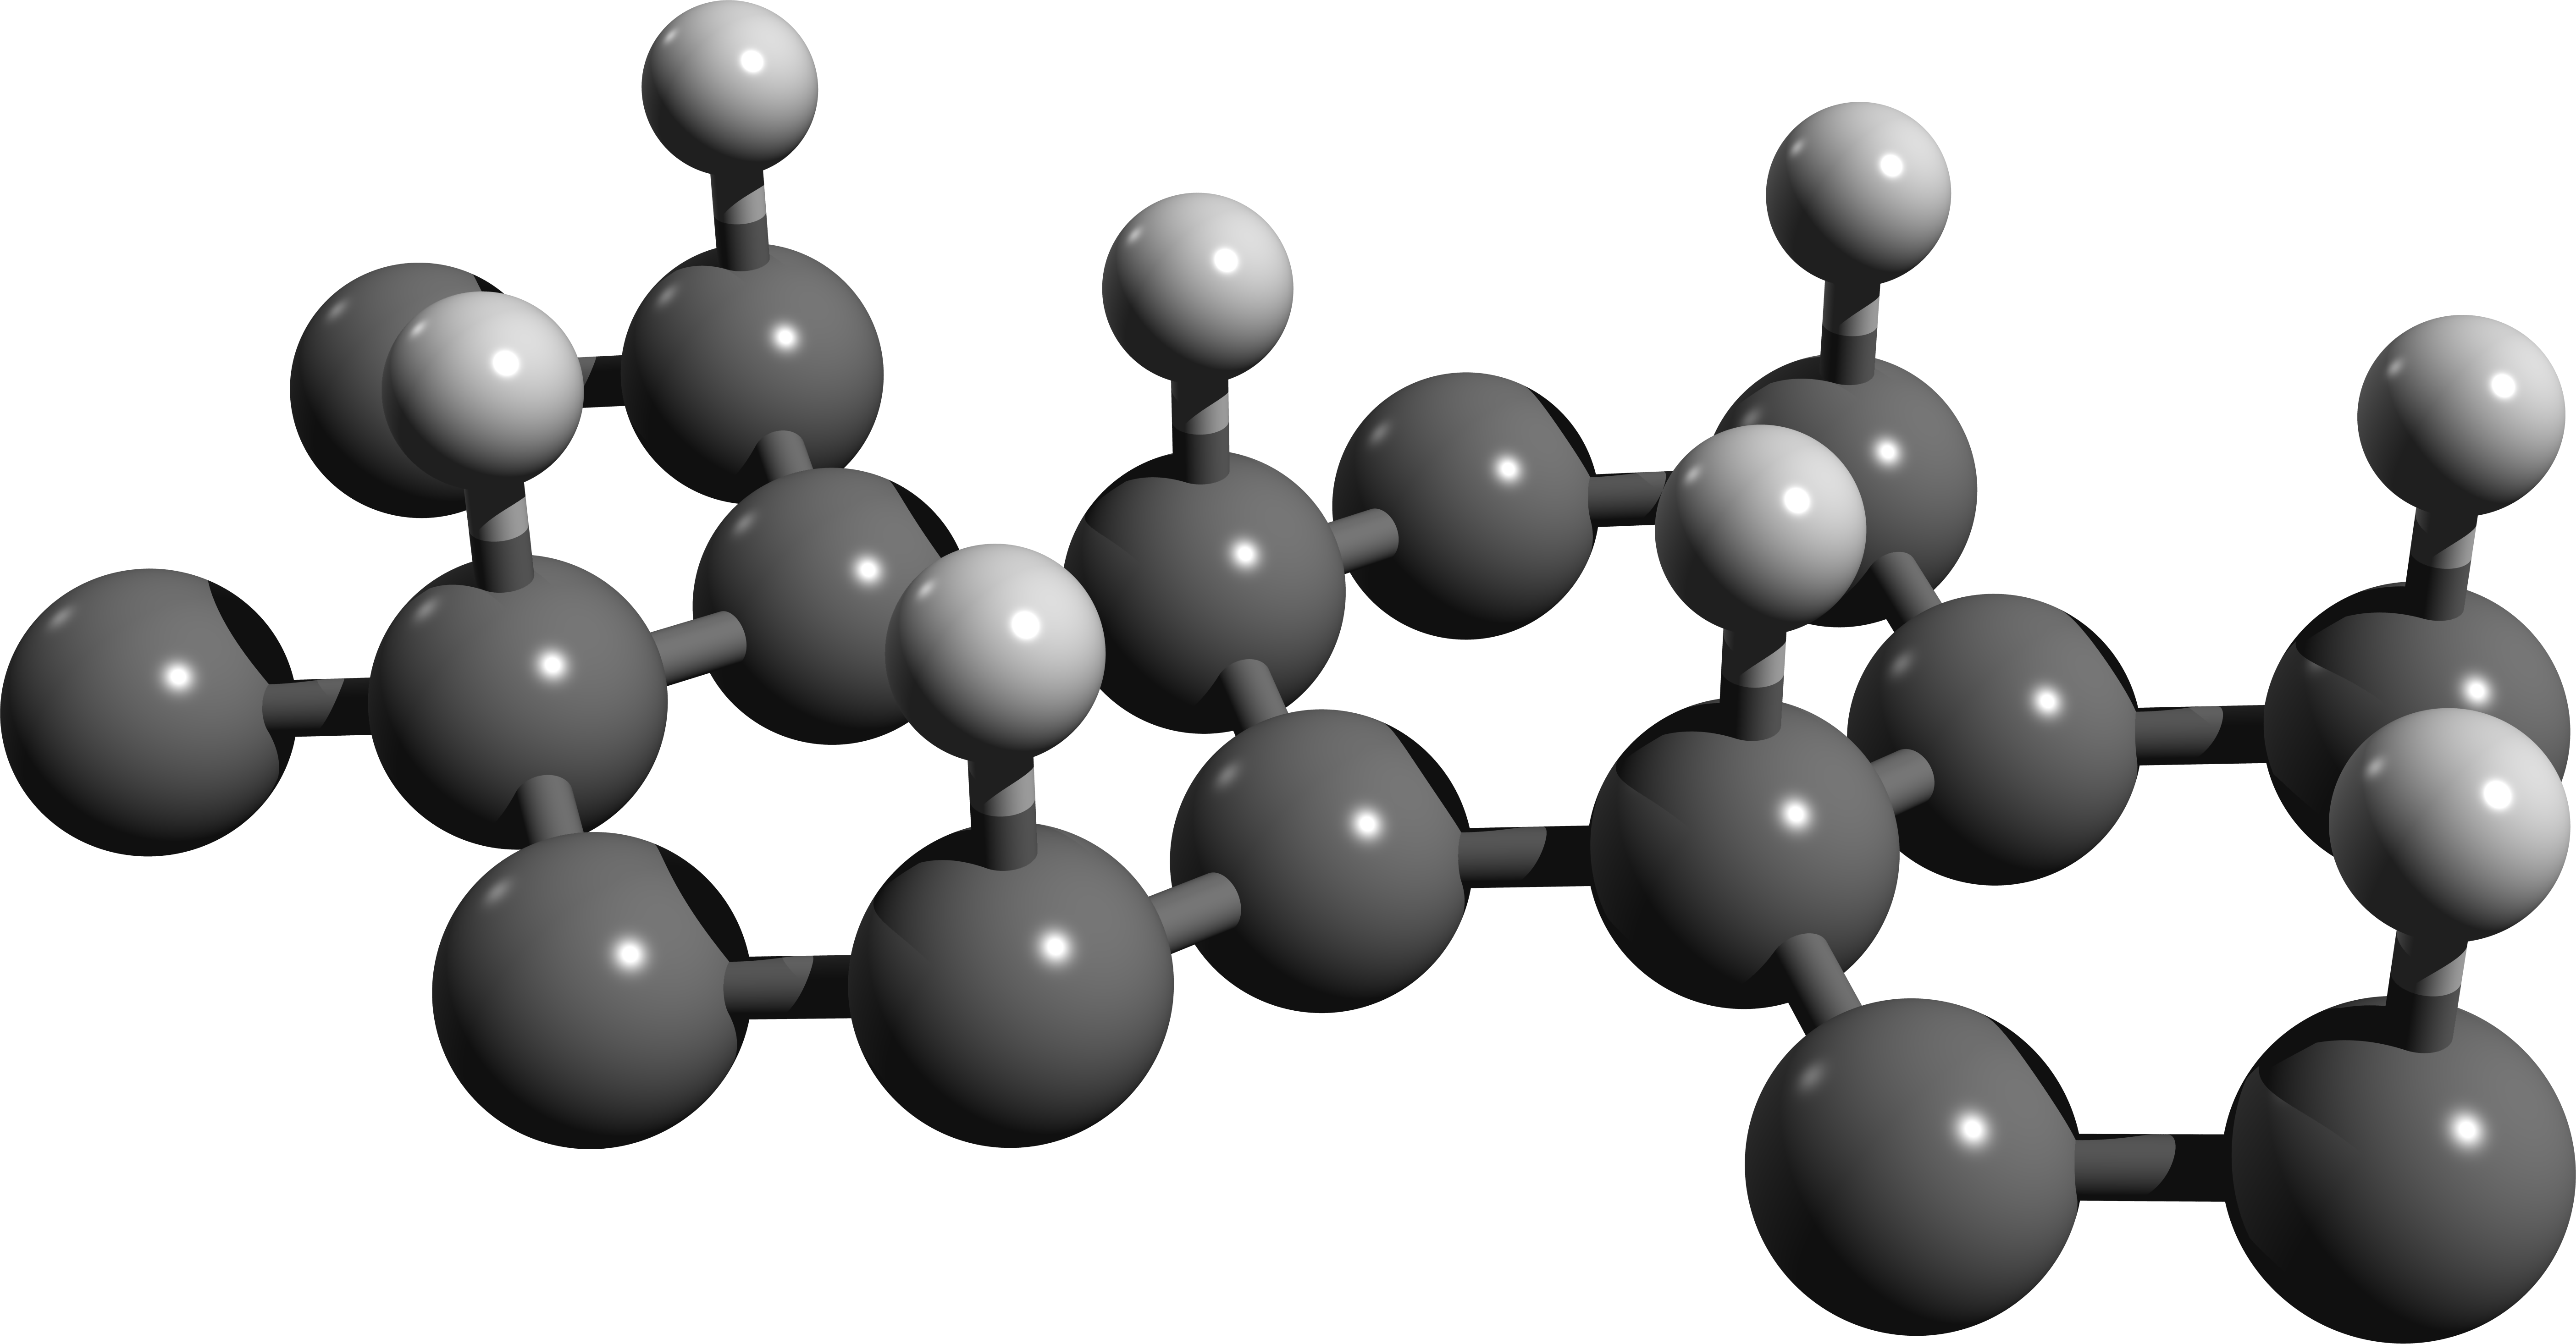
\includegraphics[width=1.0\textwidth]{figs/up3.png}};

\node[anchor=south west,inner sep=0] at (1.5, 1.4) 
{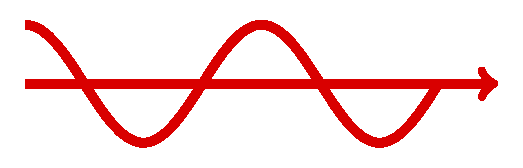
\includegraphics[width=0.55\textwidth,angle=-90,origin=c]
{figs/arrow_1omega.pdf}};

\node[anchor=south west,inner sep=0] at (1.9, 1.3) 
{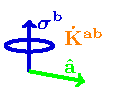
\includegraphics[width=0.40\textwidth]{figs/spin.pdf}};

\end{tikzpicture}
\end{figure}


\end{columns}

\end{frame}

%%%%%%%%%%%%%%%%%%%%%%%%%%%%%%%%%%%%%%%%%%%%%%%%%%%%%%%%%%%%%%%%%%%%%%%%%%%%%

\begin{frame}



\vspace{3mm}

\begin{itemize}

\item 
Is a second-order optical nonlinear effect.

\vspace{3mm}

\item 
A pure spin current can be produced by a single linearly polarized beam in
noncentrosymmetric materials\footnote[frame]{\tiny A. Najmaie
et. al. Phys. Rev. B, 68(16):165348, 2003.} and is given by\footnote[frame]
{\tiny Reinaldo Zapata-Pe\~na et. al. Phys. Rev. B 96, 195415. 2017}
% \vspace{-2mm}
\begin{equation}
\dot{K}^{\mathrm{ab}}(\omega) =
\mu^{\mathrm{abcd}}(\omega)
E^{\mathrm{c}}(\omega) E^{\mathrm{d*}}(\omega),
\label{eq:dotk}
\end{equation}
where $\mu^{\mathrm{abcd}}(\omega)$ is the pseudotensor that describes the rate
of change of the PSC.

\end{itemize}

\end{frame}

%%%%%%%%%%%%%%%%%%%%%%%%%%%%%%%%%%%%%%%%%%%%%%%%%%%%%%%%%%%%%%%%%%%%%%%%%%%%%

\begin{frame}

{\Large Spin velocity injection}

\vspace{6mm}

\begin{columns}

\column{0.6\textwidth}

\vspace{-8mm}
\begin{figure}[h!]
\begin{tikzpicture}

\node[anchor=south west,inner sep=0,opacity=0.40] at (0.2,-0.3) 
{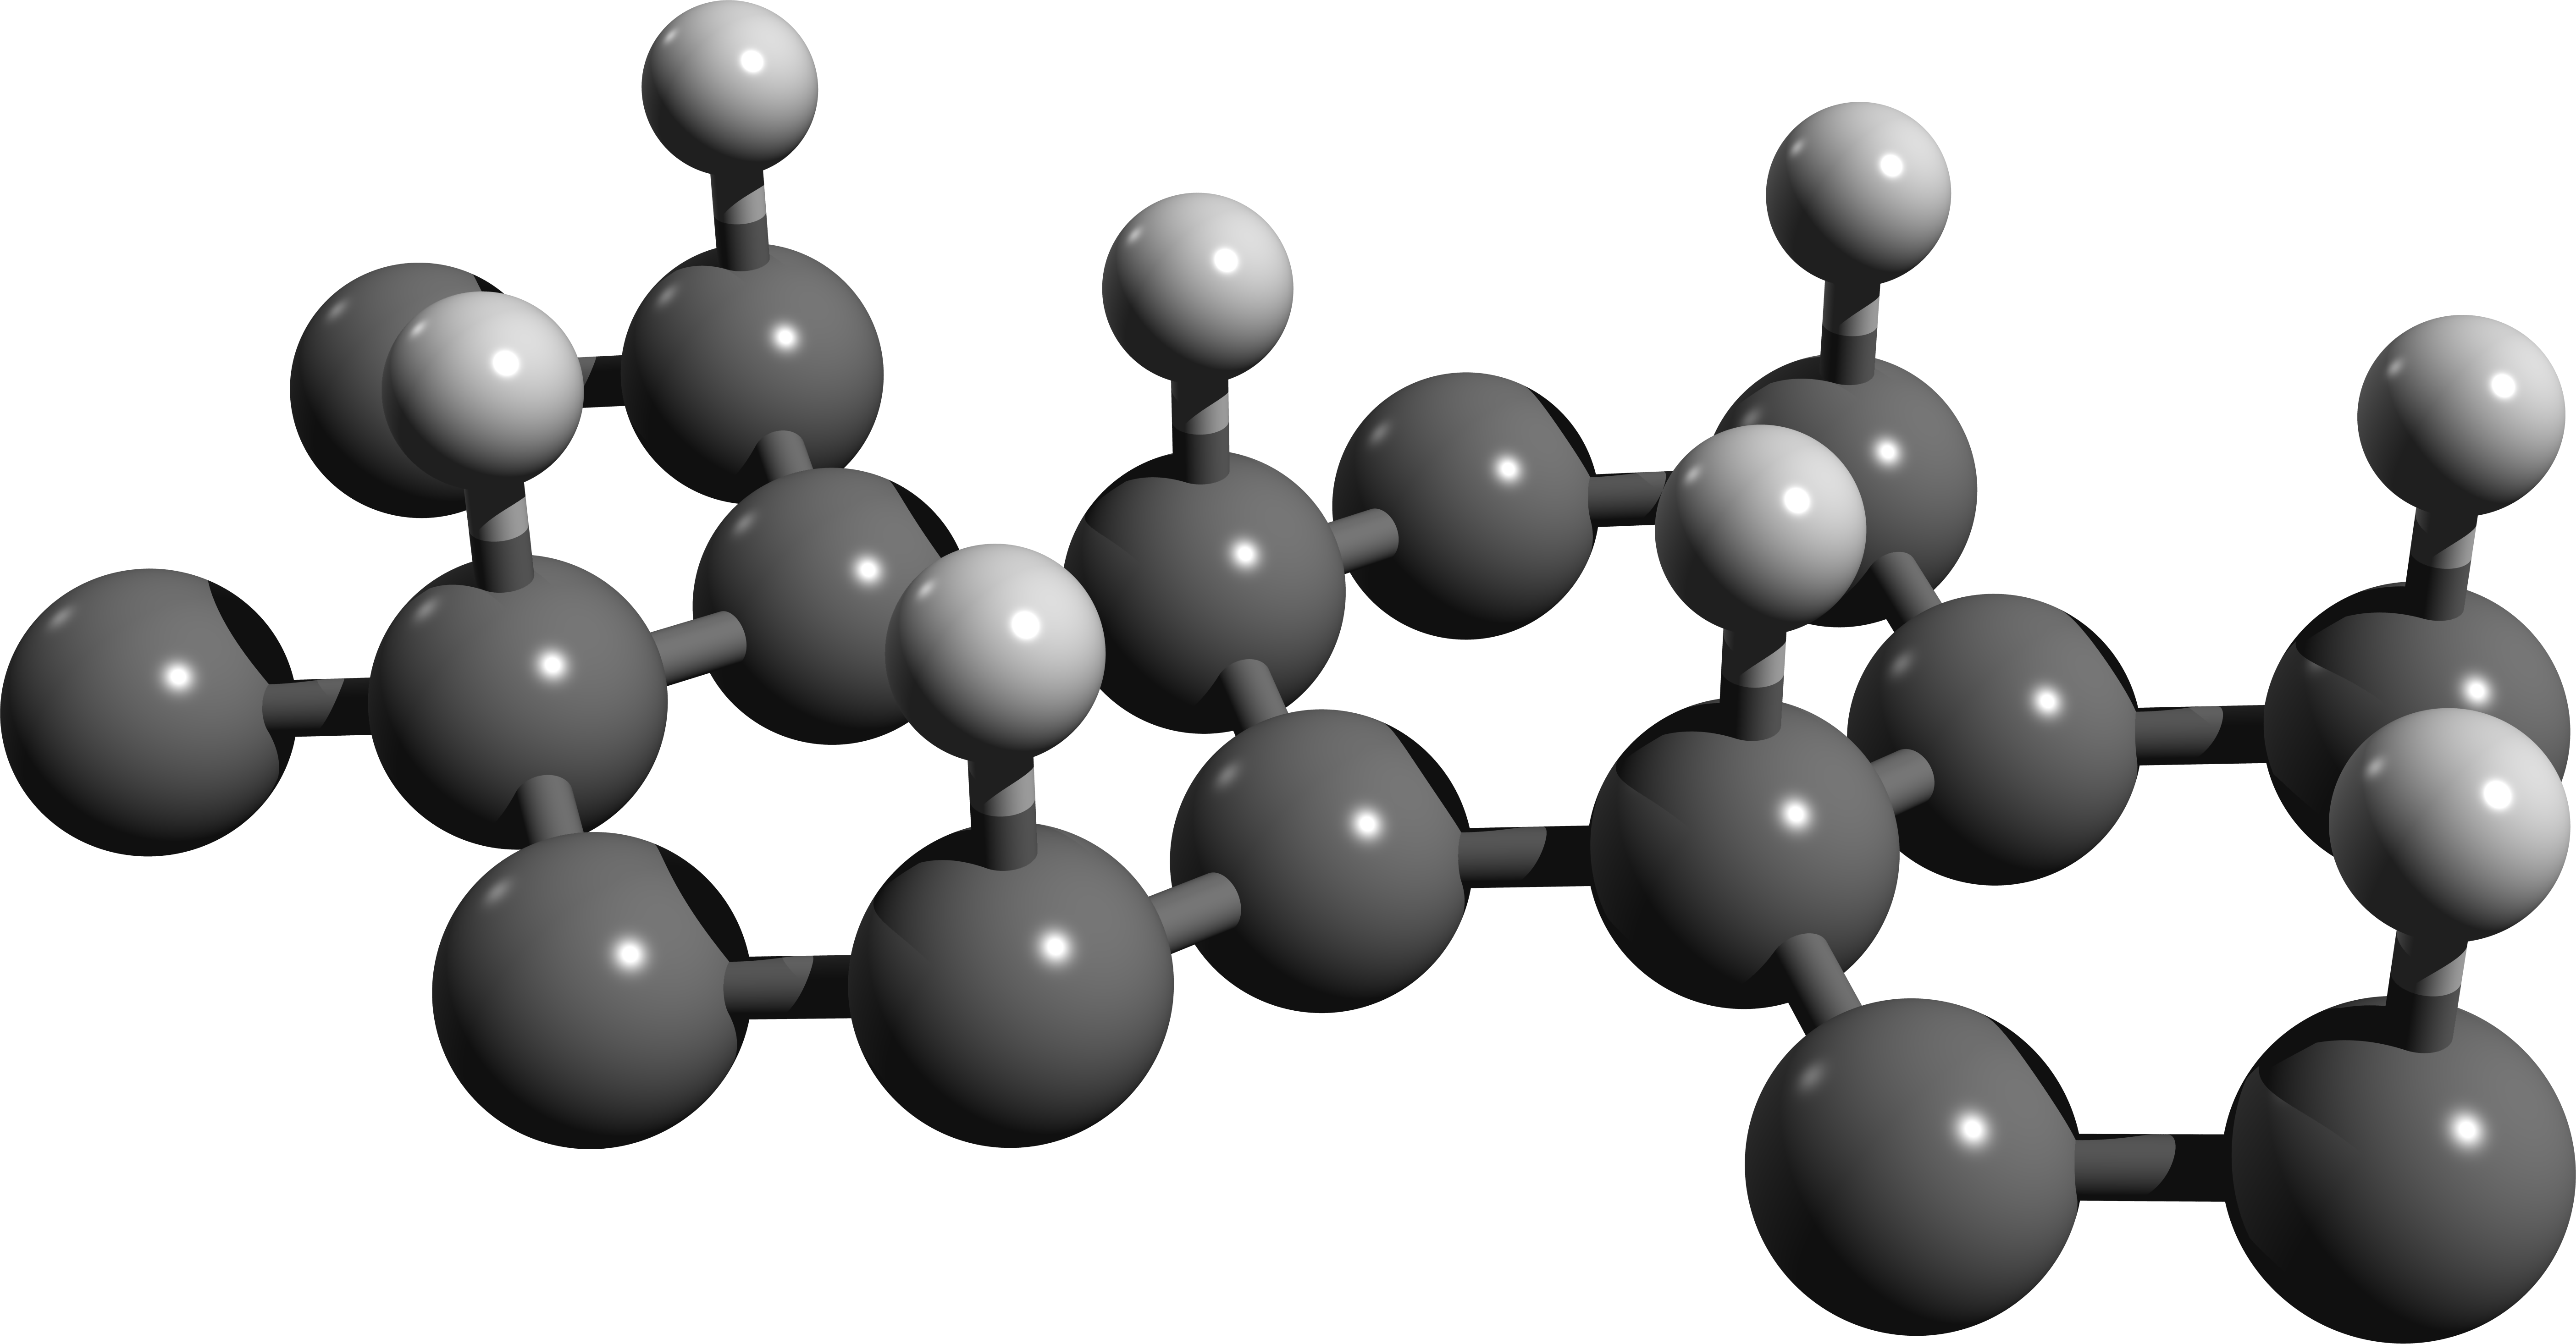
\includegraphics[width=1.0\textwidth]{figs/up3.png}};

\node[anchor=south west,inner sep=0] at (1.5, 1.4) 
{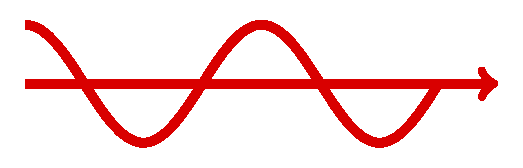
\includegraphics[width=0.55\textwidth,angle=-90,origin=c]
{figs/arrow_1omega.pdf}};

\node[anchor=south west,inner sep=0] at (2.00, 0.3) 
{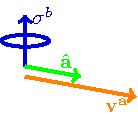
\includegraphics[width=0.6\textwidth]{figs/spinvel.pdf}};

\end{tikzpicture}
\end{figure}

\column{0.45\textwidth}

\begin{itemize}
\item 
The spin velocity injection is defined as\footnote[frame]
{\tiny Reinaldo Zapata-Pe\~na et. al. Phys. Rev. B 96, 195415. 2017}
\begin{equation}\label{eq:vab-w}
\mathcal{V}^{\mathrm{ab}}(\omega) \equiv
\frac{\dot{K}^{\mathrm{ab}}(\omega)}{(\hbar/2) \dot{n}(\omega)},
\end{equation}
which gives the velocity, along direction $\hat{\mathbf{a}}$, at which the spin
moves in a polarized state along direction $\hat{\mathbf{b}}$.
\end{itemize}

\end{columns}


\end{frame}

%%%%%%%%%%%%%%%%%%%%%%%%%%%%%%%%%%%%%%%%%%%%%%%%%%%%%%%%%%%%%%%%%%%%%%%%%%%%%

\begin{frame}

{\small

\begin{columns}

\column{0.5\textwidth}

\begin{itemize}

\item 
With 2D structures we can use the  direction of the polarized  electric field
to control ${\cal V}^{\mathrm{a}\mathrm{b}}(\omega)$.

\vspace{3mm}

\item 
Writing ${\mathbf E}(\omega) =
E_0(\omega)(\cos\alpha\,\hat{\mathbf x}+\sin\alpha\,\hat{\mathbf y})$, where
$\alpha$ is the polarization angle, we obtain that
\begin{align}
\mathcal{V}&^{\mathrm{ab}}(\omega,\alpha)
= 
\frac{2}{\hbar\xi(\omega)}
\left(\mu^{\mathrm{abxx}}(\omega)\cos^{2}\alpha + \right. \nonumber \\
&\left. \mu^{\mathrm{abyy}}(\omega)\sin^{2}\alpha + 
\mu^{\mathrm{abxy}}(\omega)\sin 2\alpha\right).
\label{eq:vab-aw}
\end{align}

\end{itemize}

\column{0.5\textwidth}

\vspace{-4mm}

\begin{figure}[h!]
\begin{tikzpicture}

\node[anchor=south west,inner sep=0] at (0.2,-1.0) 
{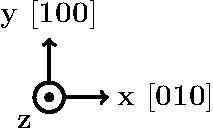
\includegraphics[width=0.4\textwidth]{figs/arrows1.pdf}};

\node[anchor=south west,inner sep=0,opacity=0.5] at (0.2,-0.3) 
{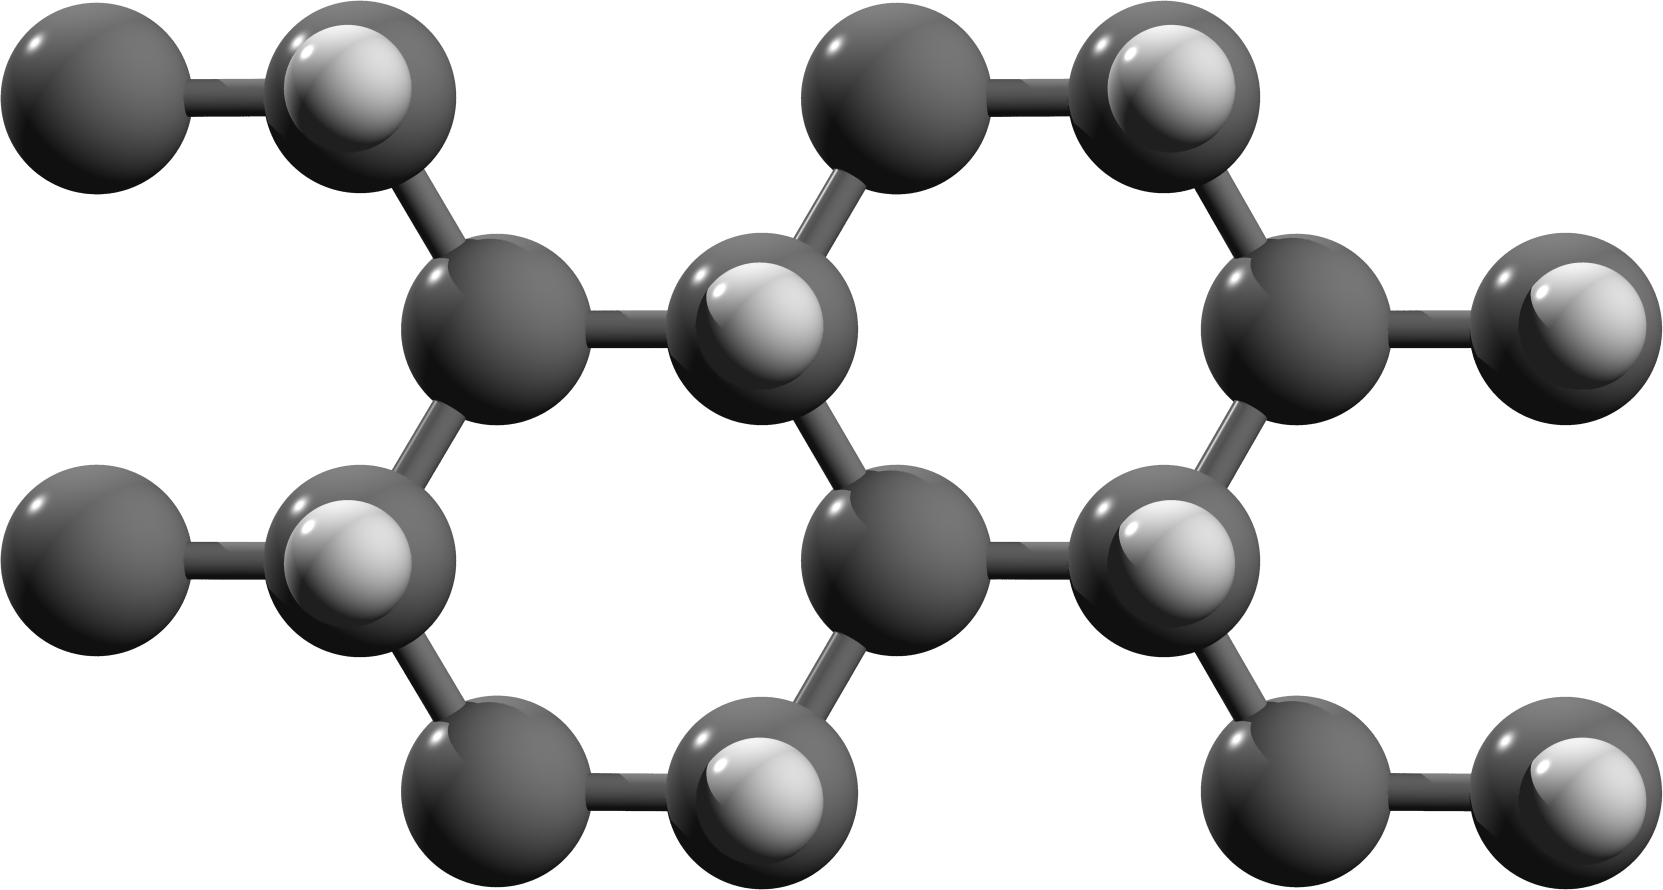
\includegraphics[width=1.0\textwidth]{figs/up1.png}};

\node[anchor=south west,inner sep=0] at (1.8,0.3) 
{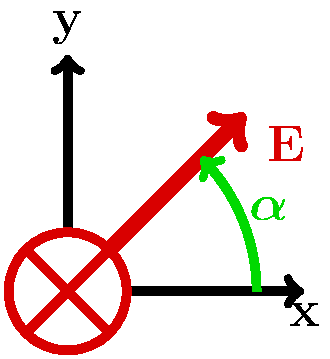
\includegraphics[width=0.40\textwidth]{figs/perp.pdf}};

\end{tikzpicture}
\end{figure}

\vspace{-14mm}

\begin{figure}[h!]
\begin{tikzpicture}


\node[anchor=south west,inner sep=0,opacity=0.5] at (0.2,-0.3) 
{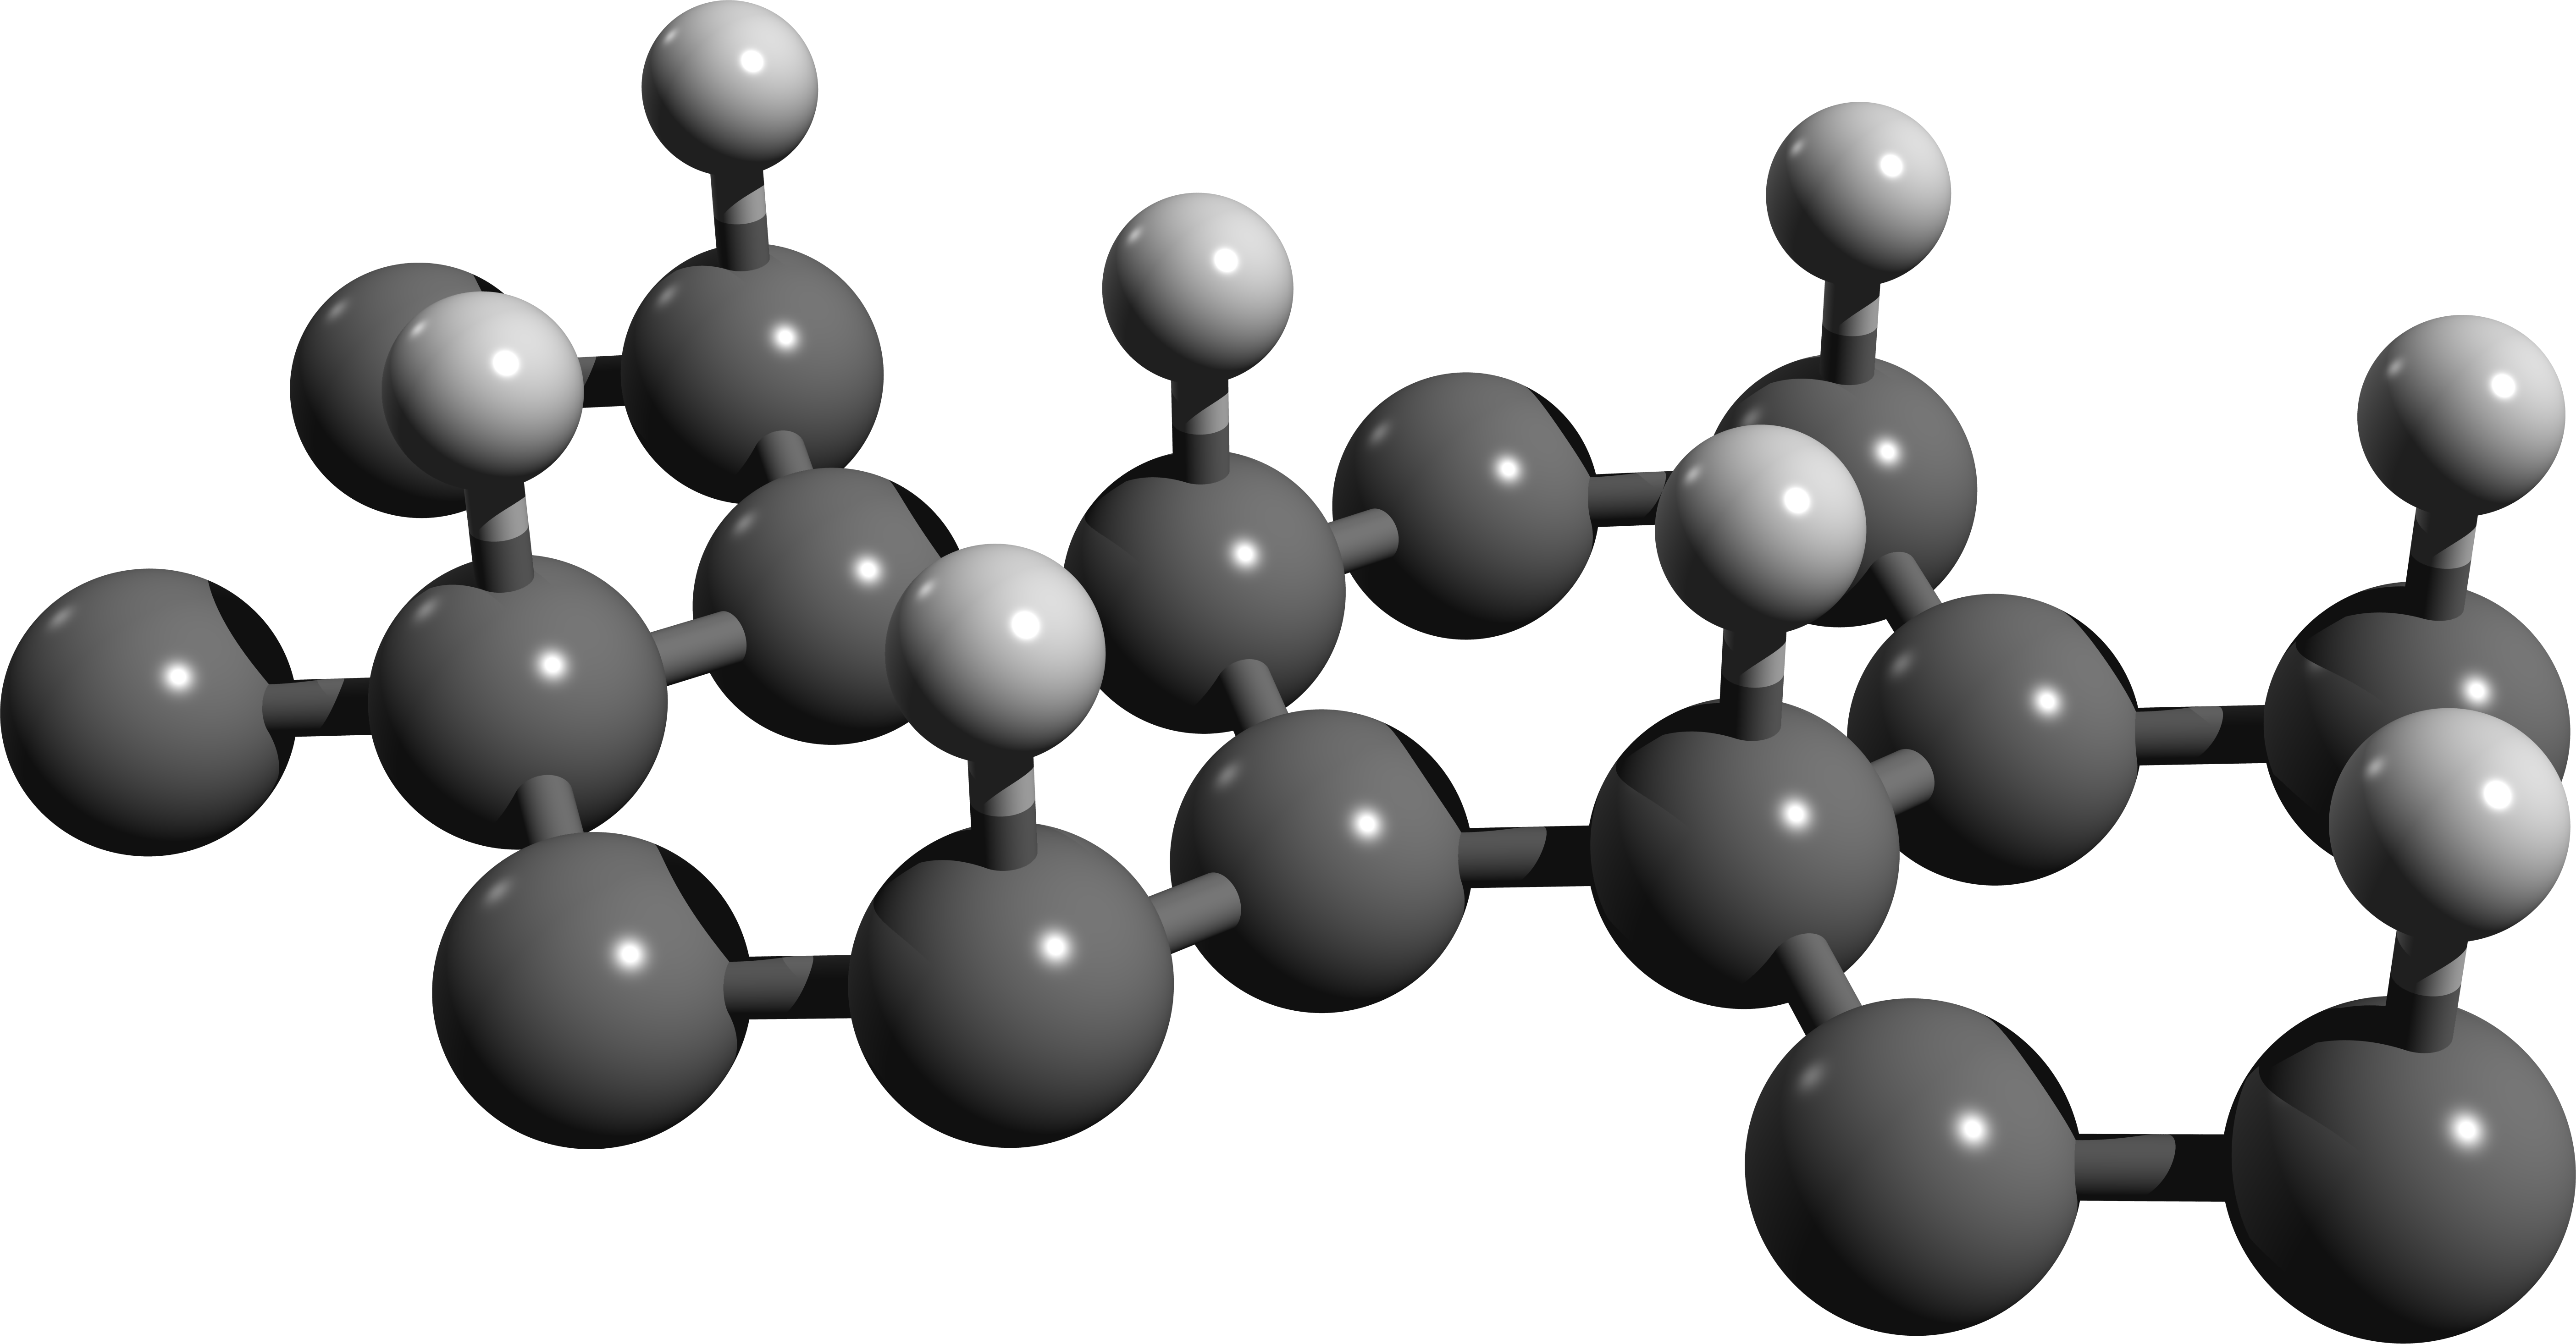
\includegraphics[width=1.0\textwidth]{figs/up3.png}};

\node[anchor=south west,inner sep=0] at (0.0,-0.7) 
{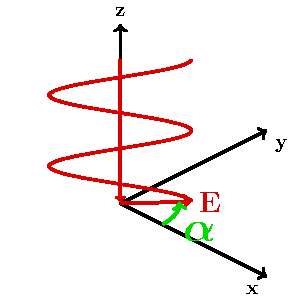
\includegraphics[width=0.8\textwidth]{figs/coord.pdf}};

\end{tikzpicture}
\end{figure}


\end{columns}

}

\end{frame}


%%%%%%%%%%%%%%%%%%%%%%%%%%%%%%%%%%%%%%%%%%%%%%%%%%%%%%%%%%%%%%%%%%%%%%%%%%%%%

%%%%%%%%%%%%%%%%%%%%%%%
\subsection{Fixing the spin polarization}
%%%%%%%%%%%%%%%%%%%%%%%

\begin{frame}

{\Large Fixing the spin polarization\footnote[frame]
{\tiny Reinaldo Zapata-Pe\~na et. al. Phys. Rev. B 96, 195415. 2017}}

{\small

\begin{columns}

\column{0.55\textwidth}

\begin{center}
{\large Spin fixed along $z$ direction}
\end{center}

\vspace{-5mm}

\begin{figure}[h!]
\begin{tikzpicture}


\node[anchor=south west,inner sep=0,opacity=0.40] at (0.2,-0.3) 
{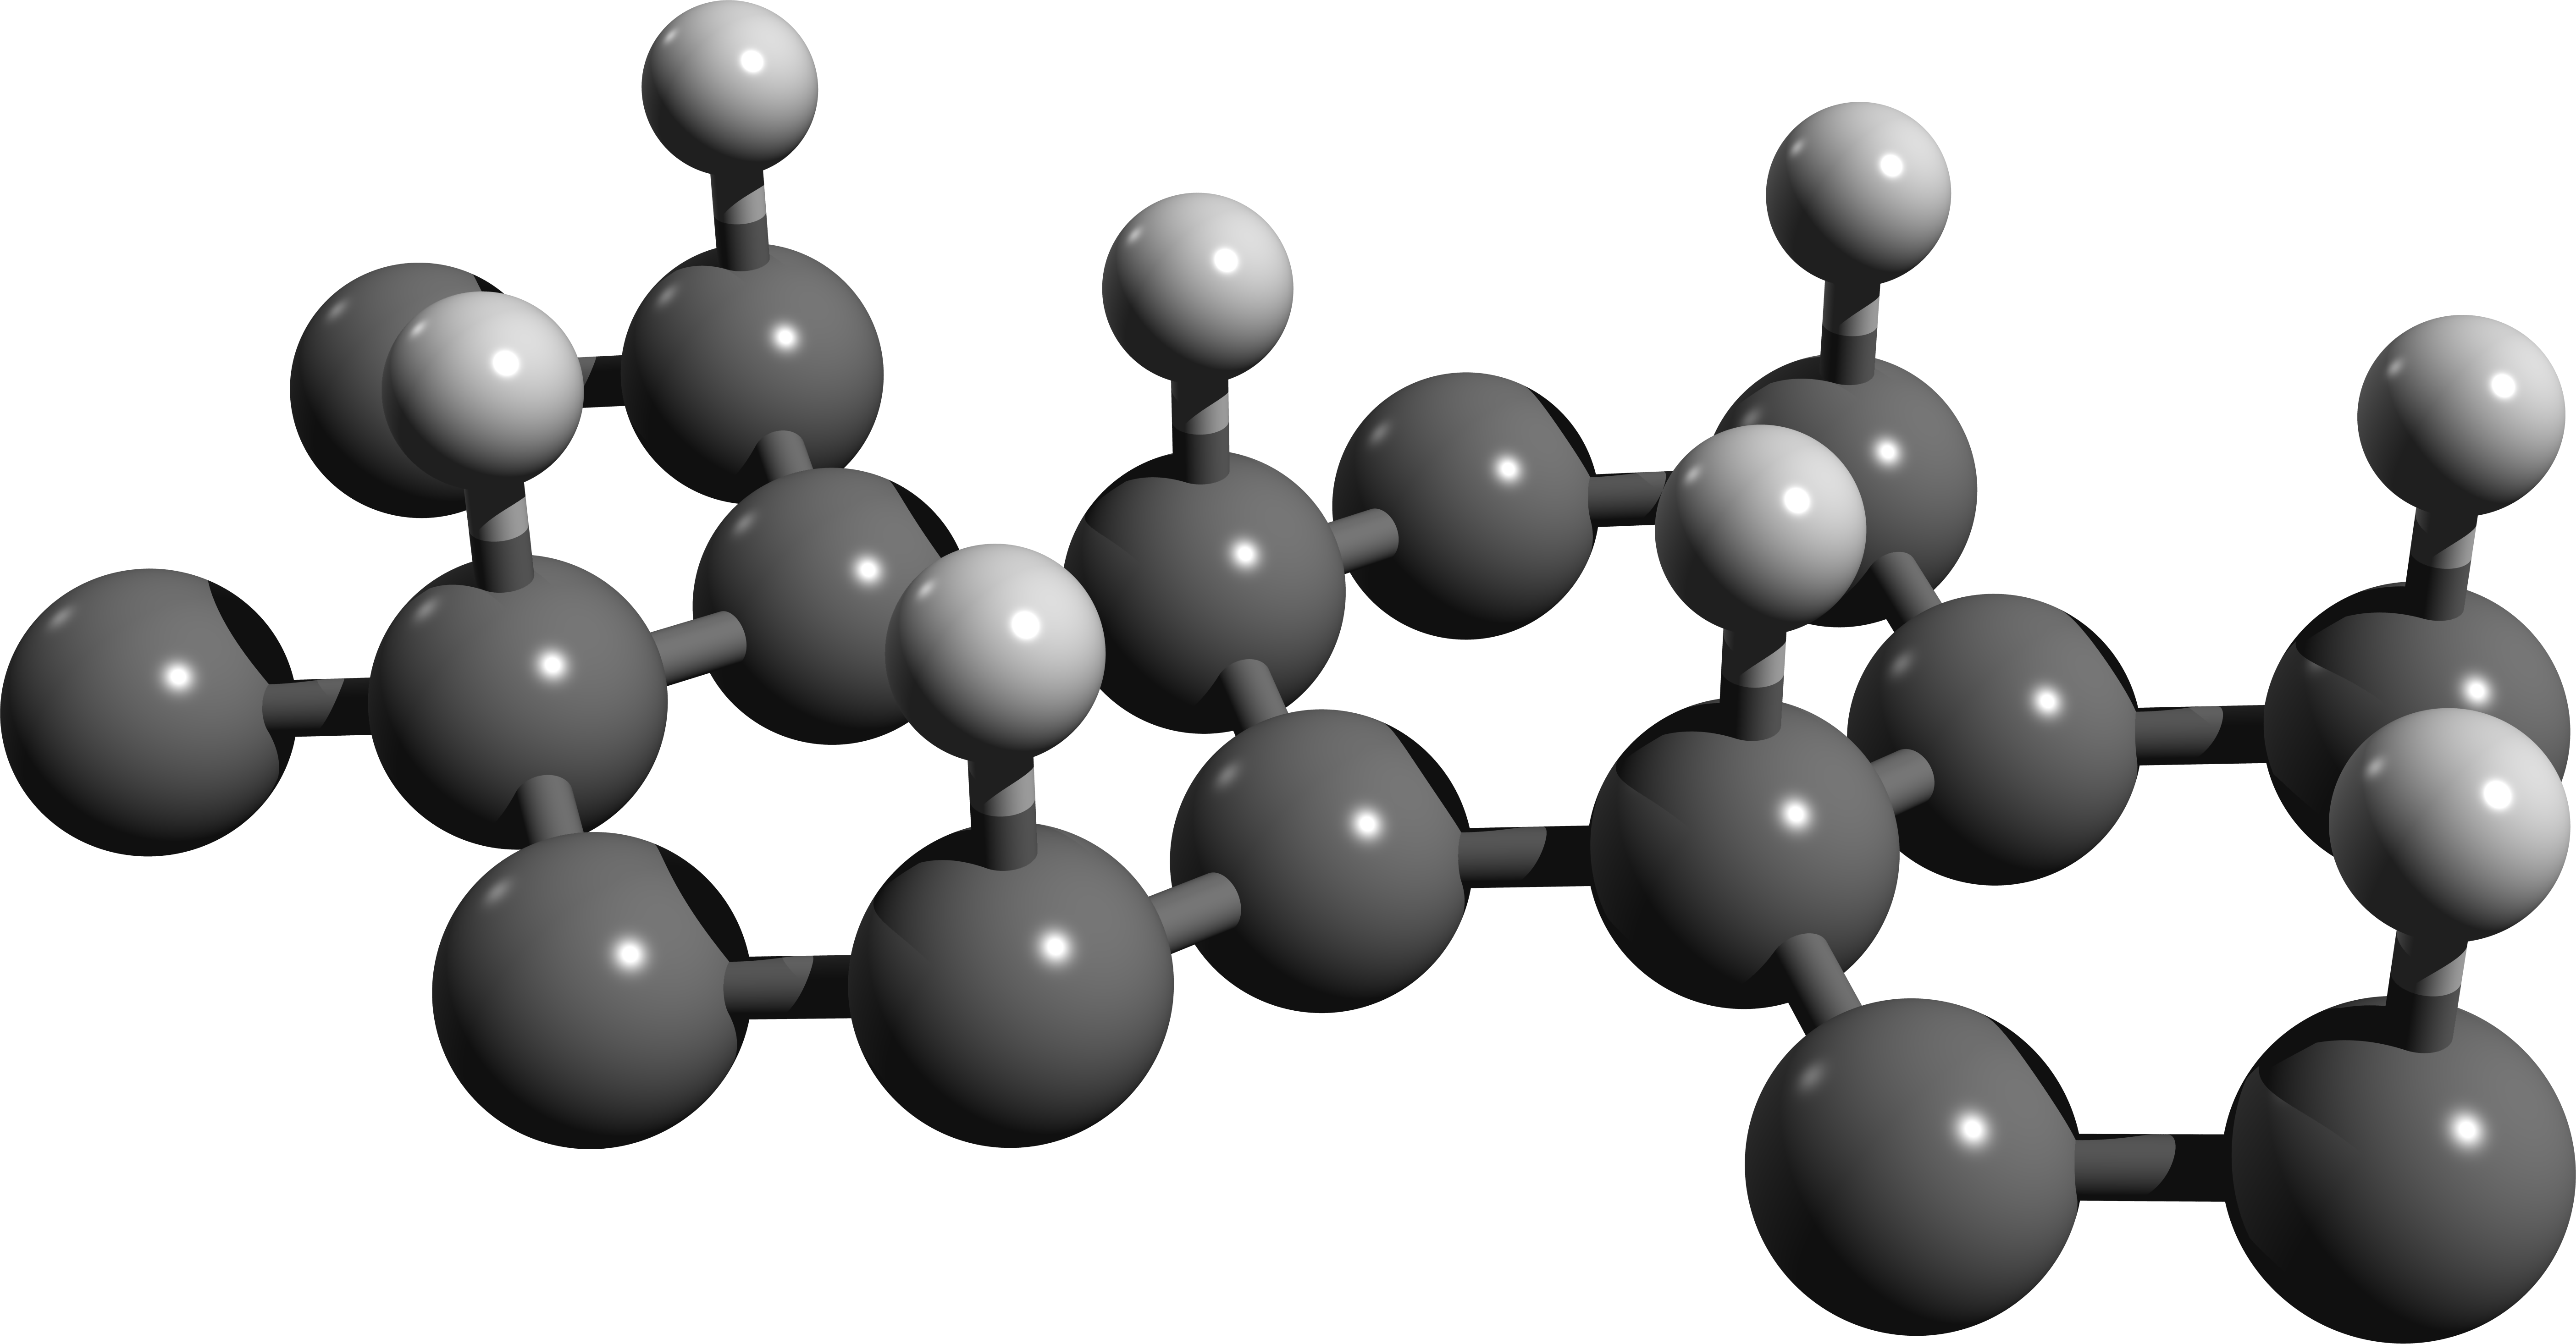
\includegraphics[width=1.0\textwidth]{figs/up3.png}};

\node[anchor=south west,inner sep=0] at (0.6,-0.4) 
{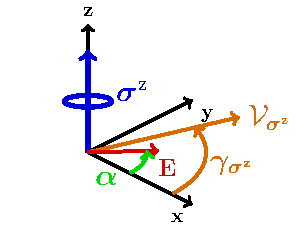
\includegraphics[width=0.85\textwidth]{figs/coord2.pdf}};

\end{tikzpicture}
\end{figure}

\column{0.5\textwidth}

\begin{itemize}

\item Magnitude of the velocity when the spin is fixed in the $\mathbf{b}$
direction 
\begin{align}
\hspace{-4mm}
\mathcal{V}_{\sigma^{\mathrm{b}}}&(\omega,\alpha)
\equiv \nonumber \\ 
&\sqrt{
\left(\mathcal{V}^{\mathrm{xb}}(\omega,\alpha)\right)^{2}\ +
\left(\mathcal{V}^{\mathrm{yb}}(\omega,\alpha)\right)^{2}\ }
\label{eq:vs-mag}
\end{align}

\item 
Angle of the velocity when the spin is fixed in the $\mathbf{b}$
\begin{equation}
\gamma_{\sigma^\mathrm{b}} (\omega,\alpha)
=
\tan^{-1} \left( \frac{\mathcal{V}^{\mathrm{yb}}(\omega,\alpha)}
{\mathcal{V}^{\mathrm{xb}}(\omega,\alpha)} \right)
\label{eq:gamma-ang}
\end{equation}

\end{itemize}
    

\end{columns}

}

\end{frame}

%%%%%%%%%%%%%%%%%%%%%%%%%%%%%%%%%%%%%%%%%%%%%%%%%%%%%%%%%%%%%%%%%%%%%%%%%%%%%

\begin{frame}

{\small

\begin{columns}

\column{0.5\textwidth}

{\Large We have two special cases}

\vspace{3mm}

\begin{itemize}

\item 
When the velocity vector is parallel to the electric incident field
\begin{equation}
\gamma_{\sigma^\mathrm{b}}^\parallel(\omega,\alpha) = \alpha, 
\label{eq:gamma-par} 
\end{equation}

\vspace{5mm}

\item 
When the velocity vector is perpendicular to the electric incident field
\begin{equation}
\gamma_{\sigma^\mathrm{b}}^\perp(\omega,\alpha) = \alpha \pm 90^{\circ},
\label{eq:gamma-perp}
\end{equation}

\end{itemize}

\column{0.55\textwidth}

\vspace{-4mm}

\begin{figure}[h!]
\begin{tikzpicture}


\node[anchor=south west,inner sep=0,opacity=0.40] at (0.2,-0.3) 
{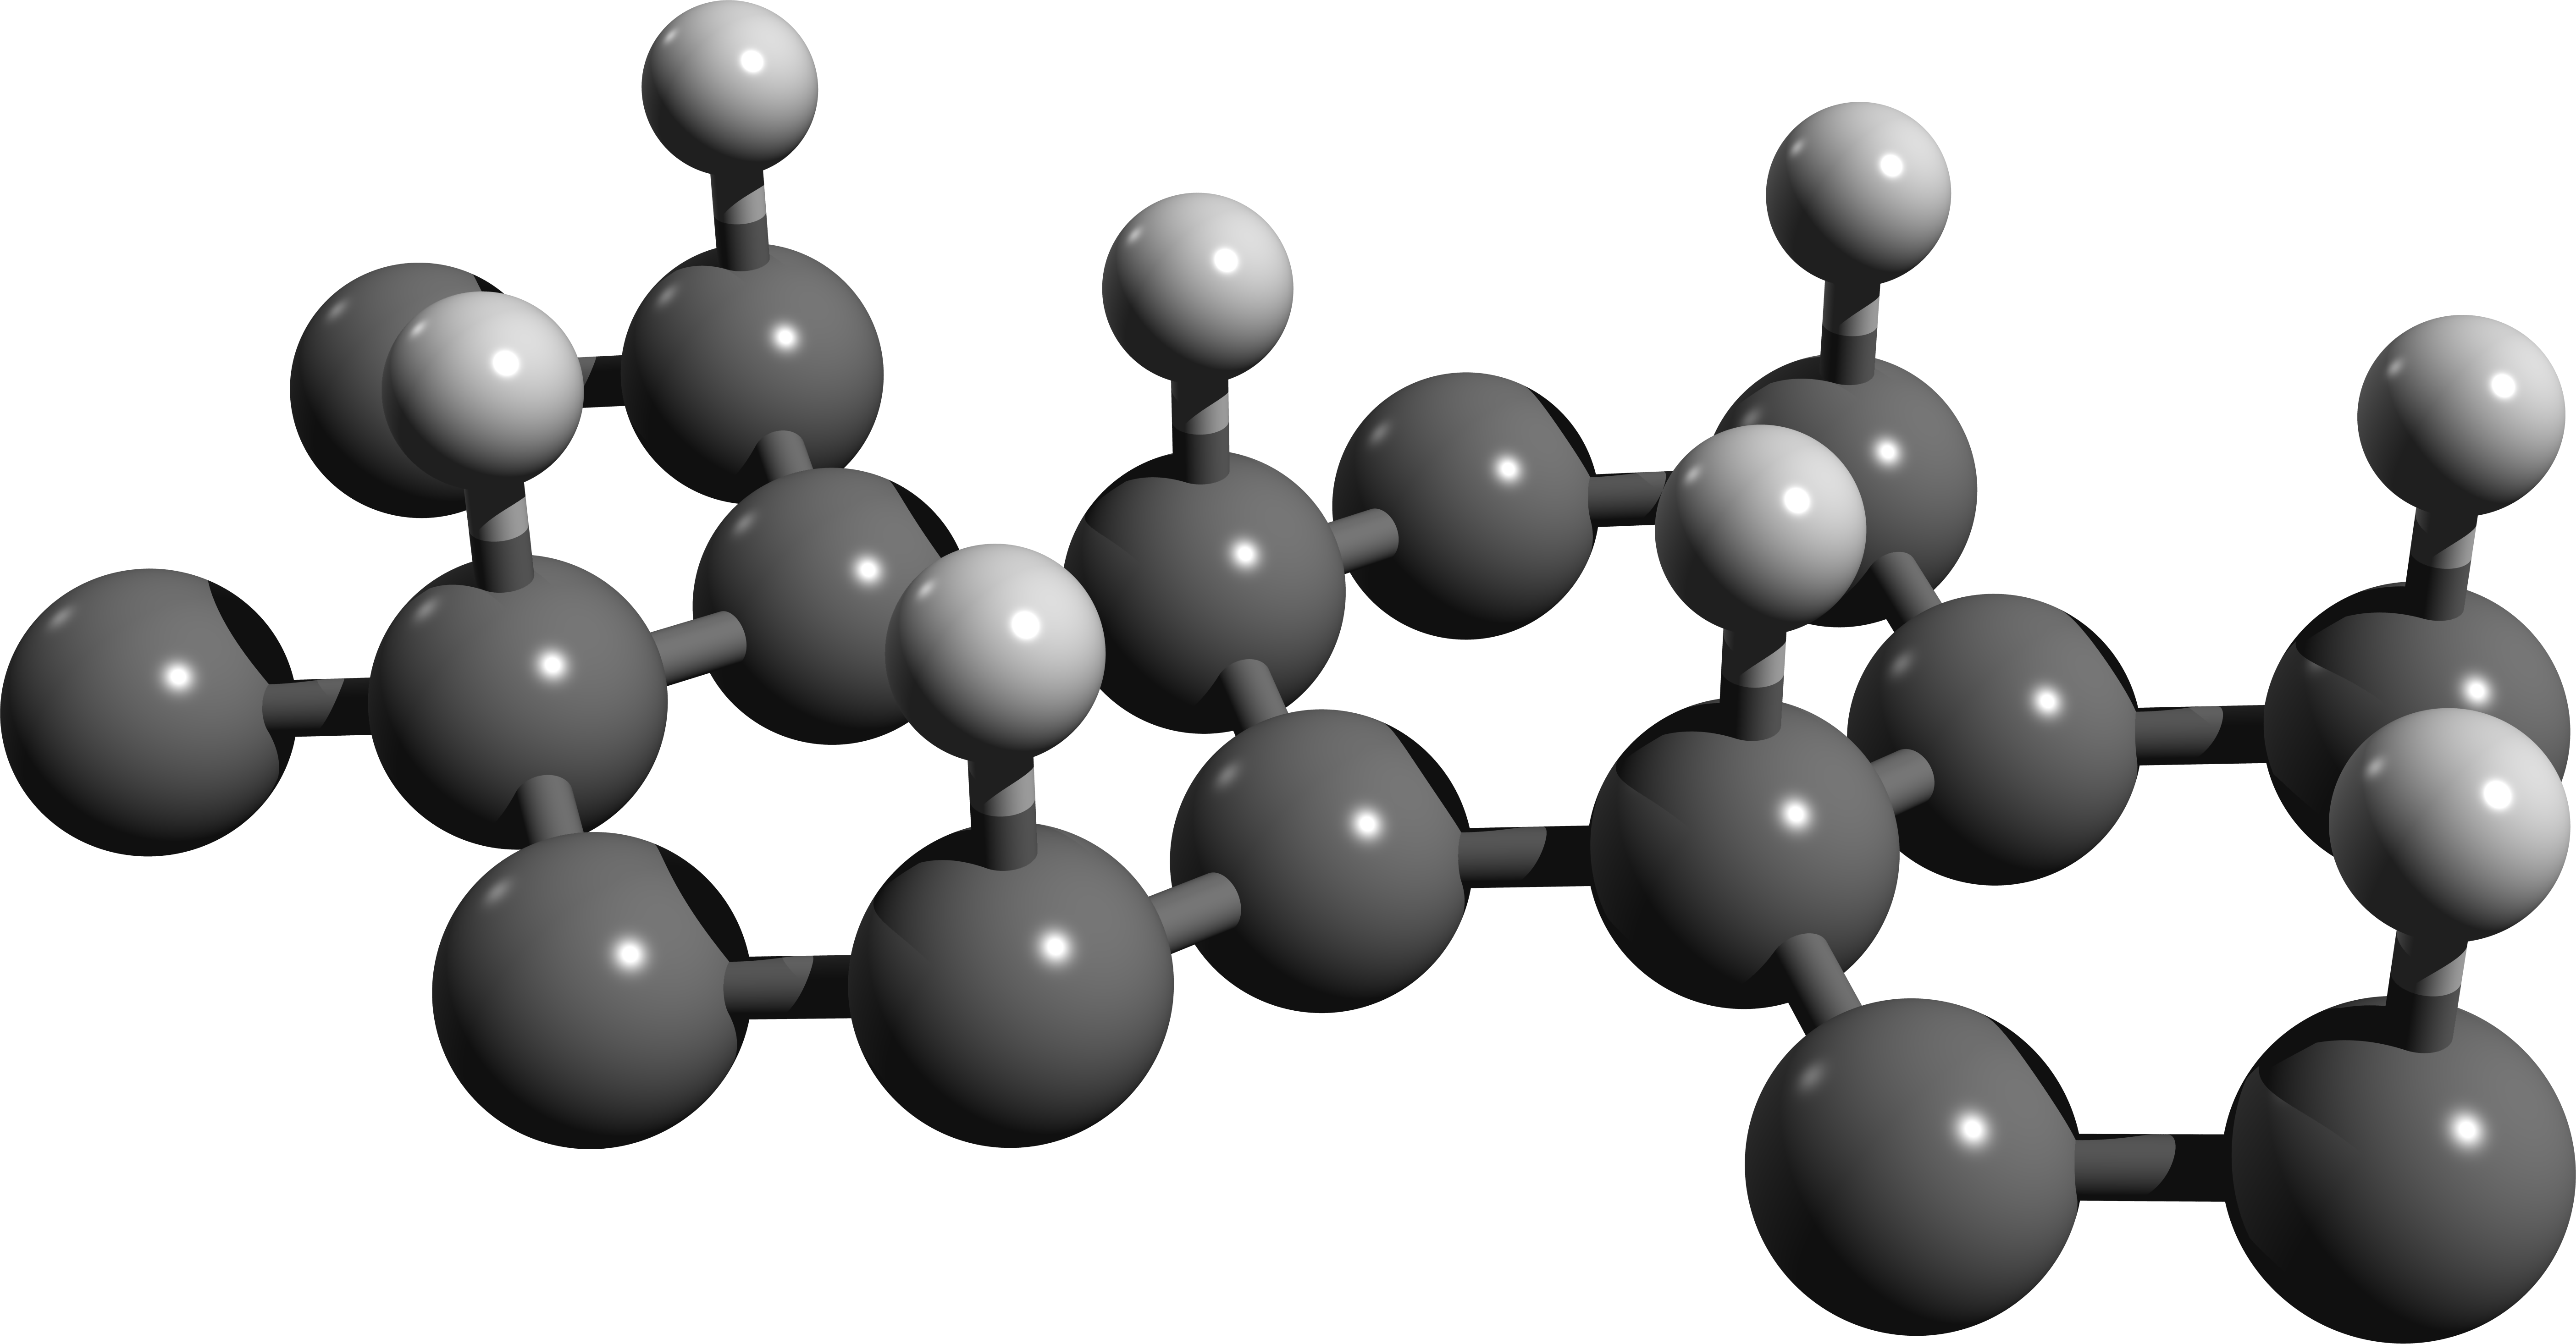
\includegraphics[width=1.0\textwidth]{figs/up3.png}};

\node[anchor=south west,inner sep=0] at (0.6,-0.3) 
{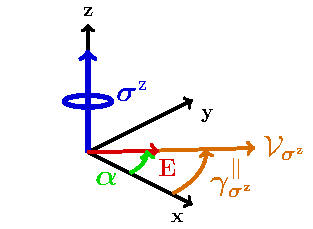
\includegraphics[width=0.85\textwidth]{figs/coord3.pdf}};

\end{tikzpicture}
\end{figure}

\vspace{-9mm}

\begin{figure}[h!]
\begin{tikzpicture}

\node[anchor=south west,inner sep=0,opacity=0.40] at (0.2,-0.3) 
{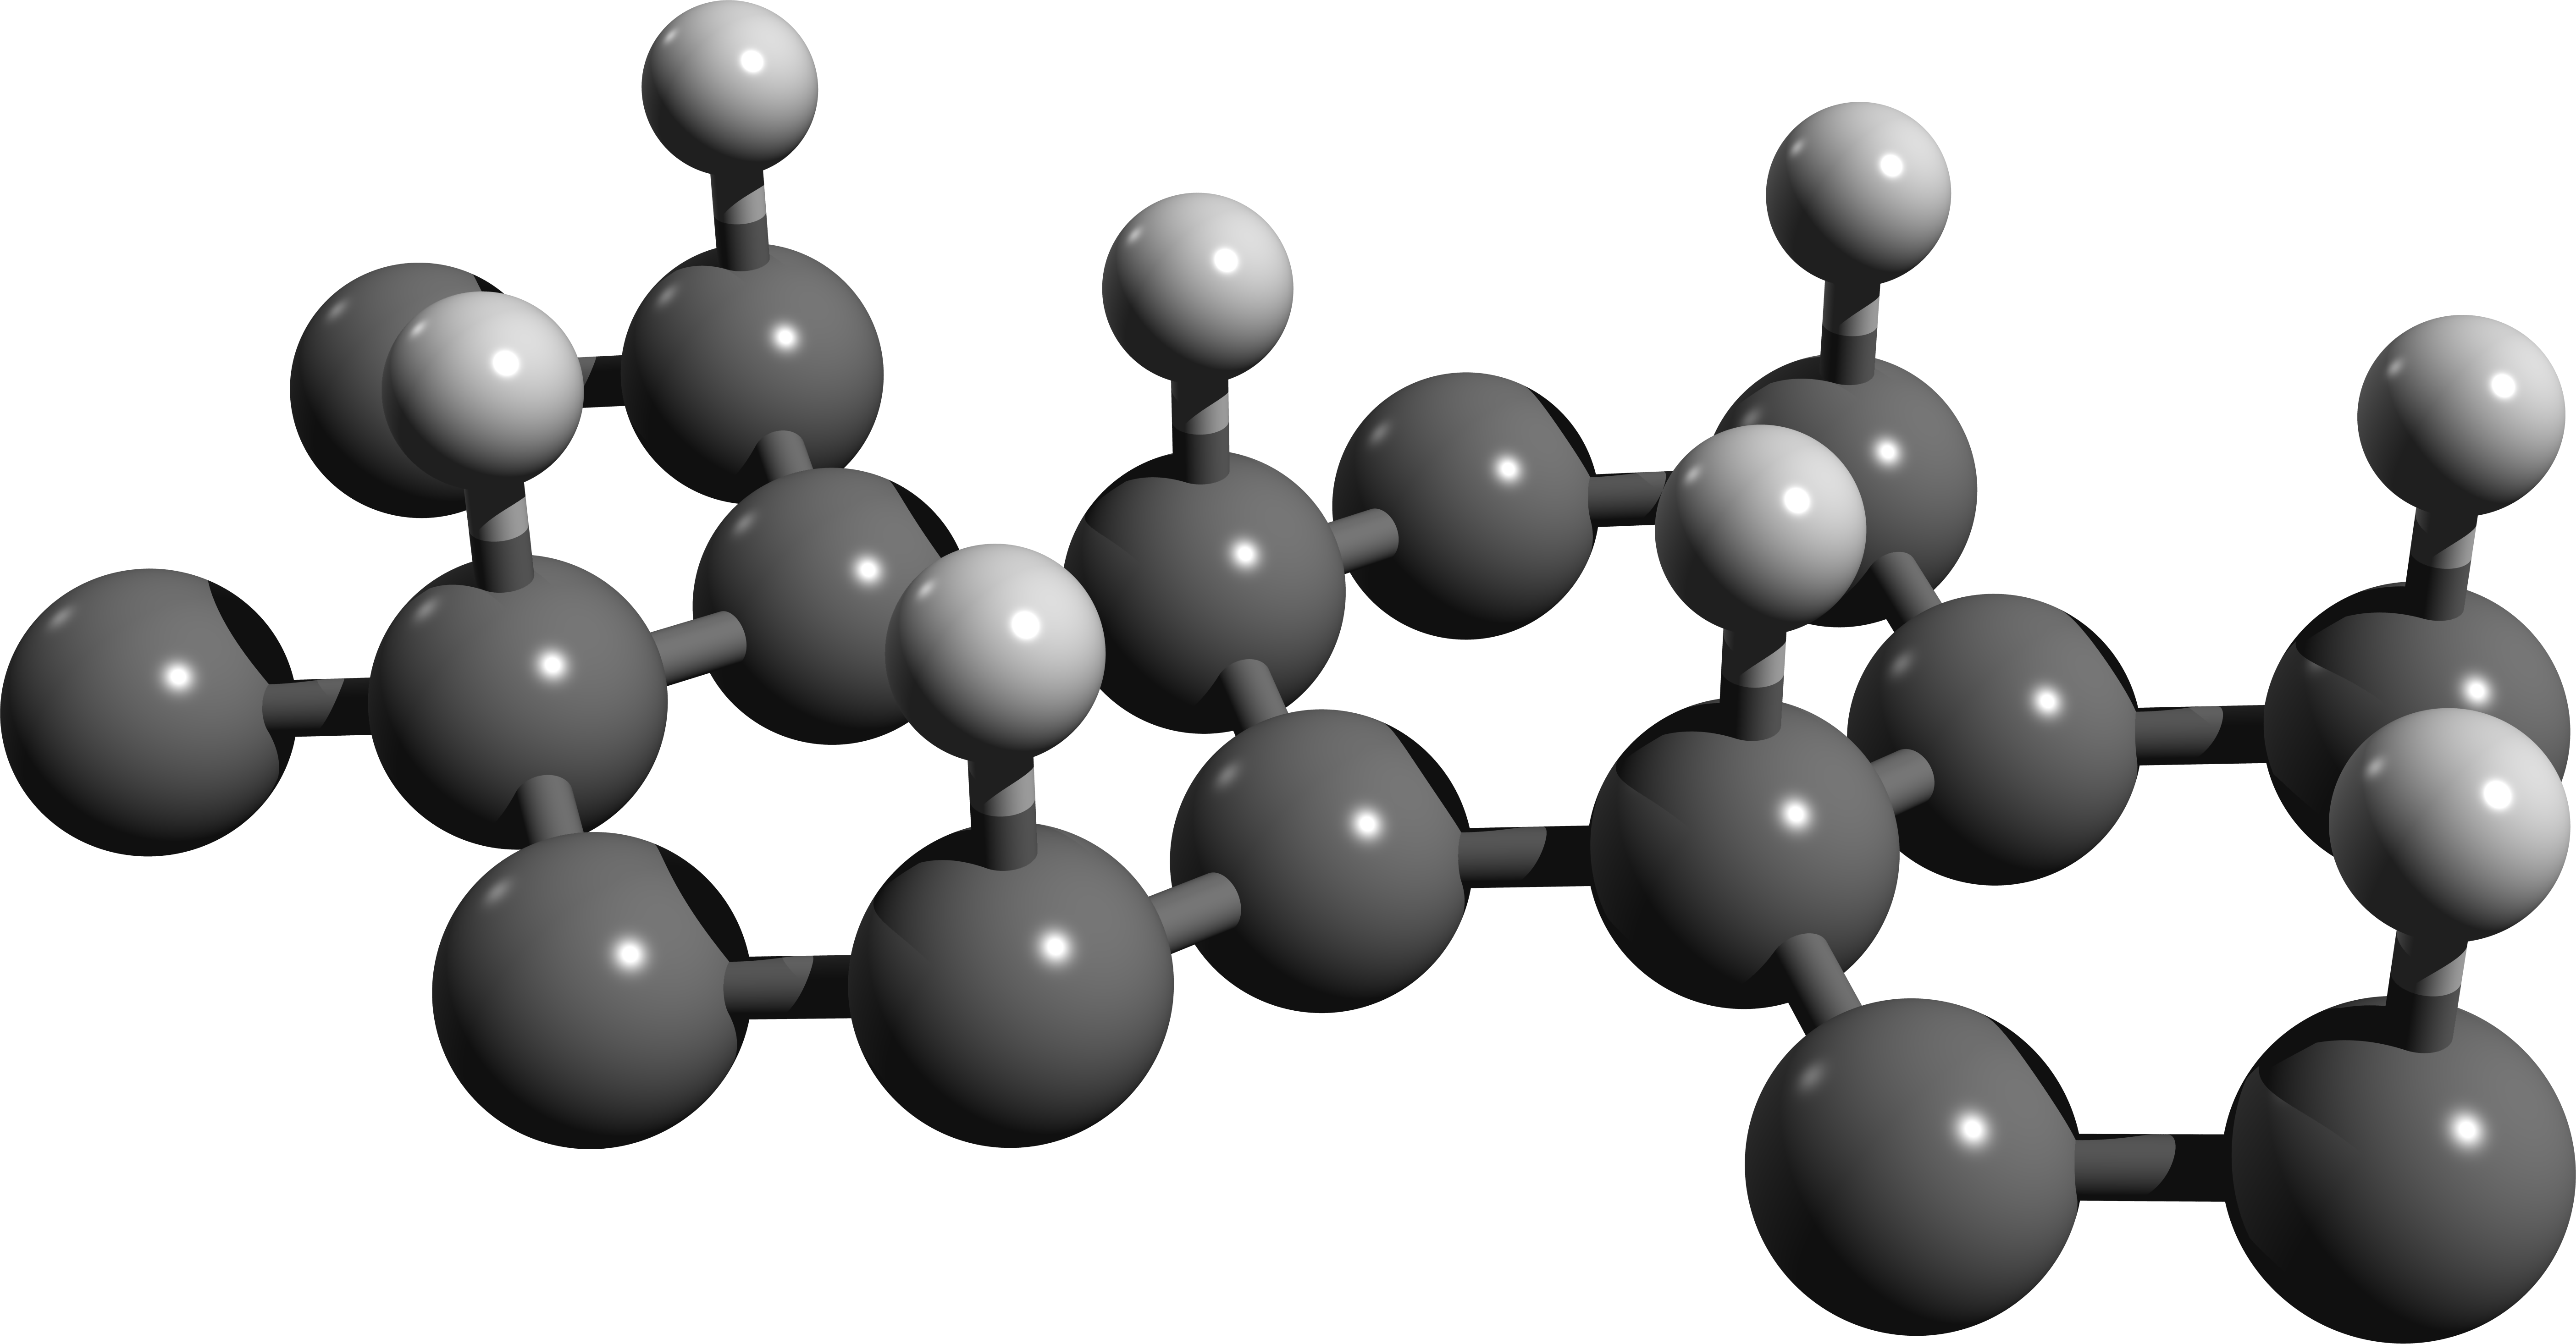
\includegraphics[width=1.0\textwidth]{figs/up3.png}};

\node[anchor=south west,inner sep=0] at (0.2,-0.6) 
{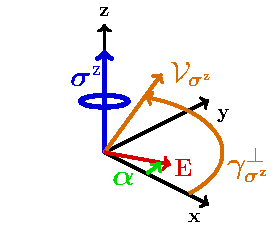
\includegraphics[width=0.85\textwidth]{figs/coord4.pdf}};

\end{tikzpicture}
\end{figure}


\end{columns}

}

\end{frame}

%%%%%%%%%%%%%%%%%%%%%%%%%%%%%%%%%%%%%%%%%%%%%%%%%%%%%%%%%%%%%%%%%%%%%%%%%%%%%

%%%%%%%%%%%%%%%%%%%%%%%
\subsection{Fixing the spin velocity}
%%%%%%%%%%%%%%%%%%%%%%%

\begin{frame}

{\Large Fixing the spin velocity\footnote[frame]
{\tiny Reinaldo Zapata-Pe\~na et. al. Phys. Rev. B 96, 195415. 2017}}


{\small

\begin{columns}

\column{0.55\textwidth}

\vspace{-5mm}

\begin{center}
{\large Velocity fixed along $y$ direction}
\end{center}

\vspace{-9mm}

\begin{figure}[h!]
\begin{tikzpicture}


\node[anchor=south west,inner sep=0,opacity=0.40] at (0.2,-0.3) 
{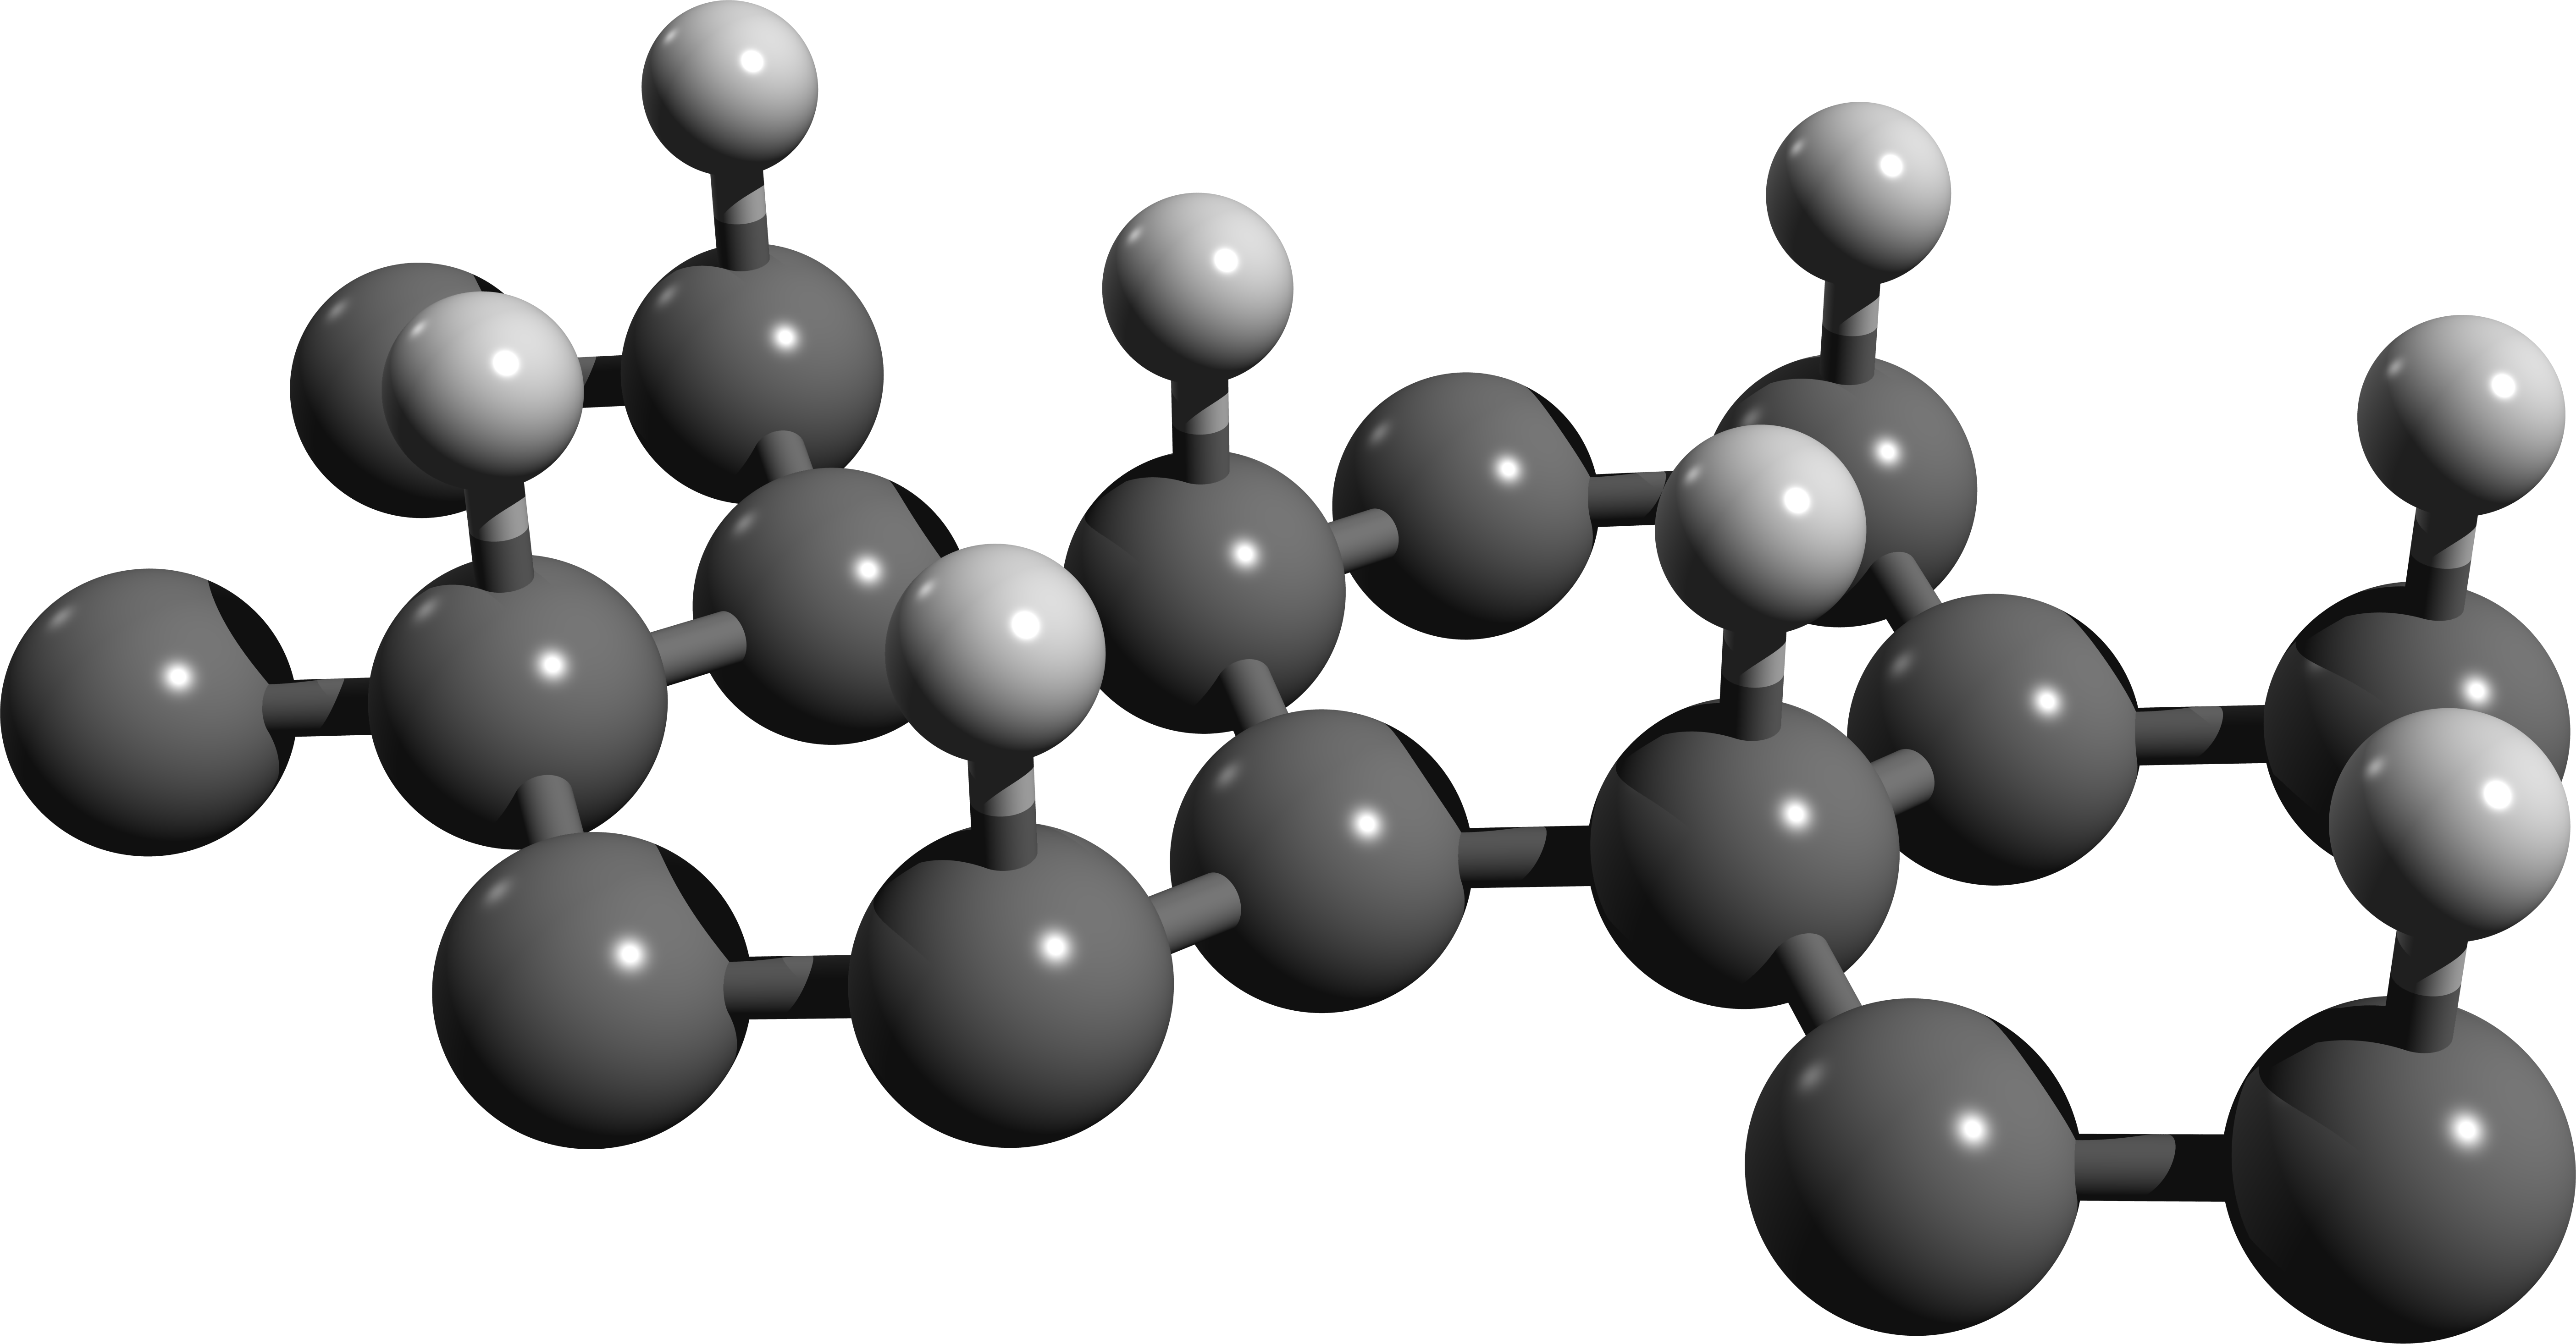
\includegraphics[width=1.0\textwidth]{figs/up3.png}};

\node[anchor=south west,inner sep=0] at (0.1,-0.7) 
{\includegraphics[width=0.85\textwidth]{figs/coord5.pdf}};

\end{tikzpicture}
\end{figure}

\column{0.5\textwidth}

\begin{itemize}

\item Magnitude of the velocity when it is fixed along $\mathbf{\hat{a}}$
direction
\vspace{-2mm}
\begin{align}
\mathcal{V}&_{\mathrm{a}}(\omega,\alpha) \equiv 
\left[
\left(\mathcal{V}^{\mathrm{ax}}(\omega,\alpha)\right)^{2} +
\right. \nonumber  \\ & \left.
\left(\mathcal{V}^{\mathrm{ay}}(\omega,\alpha)\right)^{2} +
\left(\mathcal{V}^{\mathrm{az}}(\omega,\alpha)\right)^{2} \right]
.
\label{eq:vv-mag}
\end{align}

\vspace{-5mm}

\item 
Angles of the spin

Polar angle
\vspace{-3mm}
\begin{equation}
\theta_{\mathrm{a}}  (\omega,\alpha) = 
\cos^{-1} \left( \frac{\mathcal{V}^{\mathrm{az}}(\omega,\alpha)}
{\mathcal{V}_{\mathrm{a}}(\omega,\alpha)} \right).
\label{eq:polar-ang}
\end{equation}

\vspace{-2mm}
Azimuthal angle
\vspace{-3mm}
\begin{equation}
\varphi_{\mathrm{a}} (\omega,\alpha) =
\tan^{-1} \left( \frac{\mathcal{V}^{\mathrm{ay}}(\omega,\alpha)}
{\mathcal{V}^{\mathrm{ax}}(\omega,\alpha)} \right).
\label{eq:azimuthal-ang} 
\end{equation} 

\end{itemize}
\end{columns}

}

\end{frame}


%%%%%%%%%%%%%%%%%%%%%%%%%%%%%%%%%%%%%%%%%%%%%%%%%%%%%%%%%%%%%%%%%%%%%%%%%%%%%

%%%%%%%%%%%%%%%%%%%%%%%
\subsection{Optical current injection}
%%%%%%%%%%%%%%%%%%%%%%%


\begin{frame}


\vspace{-0.2cm}

\noindent\makebox[\linewidth]{\rule{\linewidth}{0.4pt}}

\vspace{-2.0mm}
\begin{center}
{\large Optical current injection}
\end{center}

\vspace{-6mm}
\noindent\makebox[\linewidth]{\rule{\linewidth}{0.4pt}}


{\small


\begin{columns}


\column{0.6\textwidth}

\vspace{-4mm}
\begin{figure}[h!]
\begin{tikzpicture}

\node[anchor=south west,inner sep=0] at (0.2,-0.3) 
{\includegraphics[width=1.0\textwidth]{figs/up3.png}};
\node[anchor=south west,inner sep=0] at (1.9, 0.0) 
{\includegraphics[width=0.7\textwidth]{figs/helix2.pdf}};

\end{tikzpicture}
\end{figure}


\column{0.4\textwidth}

\begin{itemize}

\item 
It is possible to control a photocurrent in a bulk structure 
\footnote[frame]{\tiny A. Hache\' et. al. Phys. Rev. Lett., 78:306-309, Jan
1997.}
or in the surface of a 2D system.
\footnote[frame]{\tiny N. Arzate et al. Phys. Rev. B, 90(20):205310, 2014.}
\hspace{-1mm}\textsuperscript{,}
\footnote[frame]{\tiny R. Zapata-Pe\~na et. al. Phys. Stat. Sol. (b), 253
(2):226-233, 2016.}

\item 
Is a second-order optical nonlinear effect that can be produced with a single
optical circularly-polarized beam.\textsuperscript{ 2}


\end{itemize}


\end{columns}


}

\end{frame}

%%%%%%%%%%%%%%%%%%%%%%%%%%%%%%%%%%%%%%%%%%%%%%%%%%%%%%%%%%%%%%%%%%%%%%%%%%%%%


\begin{frame}


{\small

\begin{itemize}

\item 
A photocurrent can be injected into noncentrosymmetric materials or at the
surface of bulk centrosymmetric materials and is given by
\footnote[frame]{\tiny N. Arzate et al. Phys. Rev. B, 90(20):205310, 2014.}
\begin{equation*}
\mathbf{\dot{J}}^{a}_{\text{inj}}(\omega) =
\eta^{abc}(\omega)E_{b}(\omega)E_{c}(\omega), \label{eq:current}
\end{equation*}
where $\eta^{abc}(\omega)$ is the current injection tensor which quantifies the
current injection along the a direction $a$.

\item The response was calculated layer by layer.


\end{itemize}
}
\end{frame}

%%%%%%%%%%%%%%%%%%%%%%%%%%%%%%%%%%%%%%%%%%%%%%%%%%%%%%%%%%%%%%%%%%%%%%%%%%%%%



%%%%%%%%%%%%%%%%%%%%%%%
\subsection{Second harmonic generation}
%%%%%%%%%%%%%%%%%%%%%%%


\begin{frame}

\vspace{-0.2cm}

\noindent\makebox[\linewidth]{\rule{\linewidth}{0.4pt}}

\vspace{-2.0mm}
\begin{center}
{\large Second harmonic generation (SHG)}
\end{center}

\vspace{-6mm}
\noindent\makebox[\linewidth]{\rule{\linewidth}{0.4pt}}



\begin{columns}

\column{0.40\textwidth}

{\small


\begin{itemize}

\item 
Is a second-order optical nonlinear effect and a particular case of sum
frequency generation.

\item 
The nonlinear polarization in the media acts as a source for the
electromagnetic waves of frequency $2\omega$.

\item 
SHG spectroscopy offer a non-invasive technique to study material properties.

\end{itemize}
}

\column{0.60\textwidth}

\begin{figure}[h!]
\begin{tikzpicture}

\node[anchor=south west,inner sep=0] at (0.2,-0.3) 
{\includegraphics[width=1.0\textwidth]{figs/up3.png}};
\node[anchor=south west,inner sep=0] at (0.7, 0.8) 
{\includegraphics[width=0.55\textwidth,angle=-45,origin=c]
{figs/arrow_1omega.pdf}};
\node[anchor=south west,inner sep=0] at (3.0, 0.8) 
{\includegraphics[width=0.55\textwidth,angle=45,origin=c]
{figs/arrow_2omega.pdf}};
\draw [] (1.00, 4.10) node [right] {\Large $\omega$};
\draw [] (5.40, 4.10) node [right] {\Large $2\omega$};
\end{tikzpicture}
\end{figure}


\end{columns}

\end{frame}

%%%%%%%%%%%%%%%%%%%%%%%%%%%%%%%%%%%%%%%%%%%%%%%%%%%%%%%%%%%%%%%%%%%%%%%%%%%%%

\begin{frame}


{\small

\begin{itemize}

\item 
The second-order nonlinear polarization is given by
\footnote[frame]{\tiny S. M. Anderson et al. Phys. Rev. B, 91(7):075302, 2015.}
\begin{equation*}\label{eq:pol}
\mathcal{P}(2\omega) = 
\chi^{abc}(-2\omega;\omega,\omega)E^{b}(\omega)E^{c}(\omega),
\end{equation*} 
where $\chi^{abc}(-2\omega;\omega,\omega)$ is the nonlinear susceptibility
tensor responsible for the SHG.

\item 
The formalism includes\textsuperscript{ 1}
\begin{itemize}
\item [$-$] the scissors correction,
\item [$-$] the contribution of the nonlocal part of the pseudopotentials
\item [$-$] the cut function used to select the individual contribution for
a given layer.
\end{itemize}

\end{itemize}
}
\end{frame}

%%%%%%%%%%%%%%%%%%%%%%%%%%%%%%%%%%%%%%%%%%%%%%%%%%%%%%%%%%%%%%%%%%%%%%%%%%%%%

\begin{frame}

\begin{table}[htb]%
\centering
%\sidecaption
\begin{tabular}{lcccc}
\hline
\hline
Structure & \hspace{-5mm}Energy & \multicolumn{2}{c}{$\chi^{abc} $} &  Ref.\\
\cline{3-4} & \hspace{-5mm}[eV] & $abc$ & value \\
\hline
C$_{16}$H$_{8}$-up    &  0.04  & yxx   & $1.7\times10^{6}$ \scriptsize{pm/V}  &*     \\
C$_{16}$H$_{8}$-alt   &  0.44  & xyy   & $3\times10^{3}$\,\scriptsize{pm/V}  & *     \\
Si(100)2$\times$1     &  1.82  & xxx   & 660\, \scriptsize{pm/V}  & 
\textsuperscript{\ref{ft:andersonPRB15}}  \\
BNNT(6,0) pristine    &  5.00  & zzz   & 35\,  \scriptsize{pm/V}  & 
\footnote[frame]{\tiny R. V. Salazar-Aparicio et. al Phys. Rev. B, 90
(15):155403, 2014. \label{ft:salazarPRB14}} \\
BNNT(6,0)+4(H$_{2}$)  &  5.00  & zzz   & 33\,  \scriptsize{pm/V}  & 
\textsuperscript{\ref{ft:salazarPRB14}} \\
BNNT(6,0)+12(H$_{2}$) &  4.80  & zzz   & 15\,  \scriptsize{pm/V}  &
\textsuperscript{\ref{ft:salazarPRB14}} \\
GaAs(001)     &  3.00  & xyz   & 750\, \scriptsize{pm/V}  & 
\footnote[frame]{\tiny S. Bergfeld et. al. Phys. Rev. Lett., 90(3):036801,
2003.} \\
\hline
\hline
\end{tabular}
\caption[]{%
Comparison of the highest reported absolute values of SHG for 
different structures and components. ($^{*}$This work.)}
\label{tab:shgcomp}
\end{table}


\end{frame}

%%%%%%%%%%%%%%%%%%%%%%%%%%%%%%%%%%%%%%%%%%%%%%%%%%%%%%%%%%%%%%%%%%%%%%%%%%%%%



%%%%%%%%%%%%%%%%%%%%%%%%%%%%%%%%%%%%%%%%%%%%%%%%%%%%%%%%%%%%%%%%%%%%%%%%%%%%%
\section{Pure Spin Current Injection in Hydrogenated Graphene Structures} 
%%%%%%%%%%%%%%%%%%%%%%%%%%%%%%%%%%%%%%%%%%%%%%%%%%%%%%%%%%%%%%%%%%%%%%%%%%%%%



%%%%%%%%%%%%%%%%%%%%%%%
\subsection{Spin velocity injection}
%%%%%%%%%%%%%%%%%%%%%%%


\begin{frame}

\vspace{-0.7cm}

\noindent\makebox[\linewidth]{\rule{\linewidth}{0.4pt}}

\vspace{-2.0mm}
\begin{center}
{\large Pure Spin Current Injection in \\Hydrogenated Graphene Structures}
\end{center}

\vspace{-6mm}
\noindent\makebox[\linewidth]{\rule{\linewidth}{0.4pt}}

\vspace{2mm}

{\small

\begin{itemize}

\item 
The spin velocity injection (SVI) resulting from the pure spin current (PSC).

\item 
To calculate the velocity of the spin injection ${\cal
V}^{\mathrm{a}\mathrm{b}}(\omega)$ along direction $\hat{\mathbf{a}}$ at which
the spin moves in a polarized state along direction $\hat{\mathbf{b}}$, we
start with the operator that describes the electronic SVI, written as
\begin{equation}
\dot{K}^{\mathrm{ab}}(\omega) =
\mu^{\mathrm{abcd}}(\omega)
E^{\mathrm{c}}(\omega) E^{\mathrm{d*}}(\omega),
\label{eq:dotk}
\end{equation}

\end{itemize}
}
\end{frame}

%%%%%%%%%%%%%%%%%%%%%%%%%%%%%%%%%%%%%%%%%%%%%%%%%%%%%%%%%%%%%%%%%%%%%%%%%%%%%

\begin{frame}

{\small


\begin{itemize}

\item 
The pseudotensor of the response is given by
\begin{equation}\label{eq:mu}
\begin{aligned}
\mu^{\mathrm{abcd}}  (\omega) 
=&
\frac{\pi e^{2}}{\hbar^{2}} \int 
\frac{d^{3}k}{8 \pi^{3}} \sum'_{vcc'}
\delta(\omega-\omega_{cv}({\mathbf k})  \\
&\mathrm{Re} \left[ K^{\mathrm{ab}}_{cc'}({\mathbf k}) 
\left(  
r^{\mathrm{c}}_{vc'}({\mathbf k})   
r^{\mathrm{d}}_{cv }({\mathbf k})  +
(c \leftrightarrow d)  
\right) 
\right]
\end{aligned}
\end{equation} 

and since $\mu^{\mathrm{abcd}}(\omega)$ is
real, we have that $\mu^{\mathrm{abcd}}(\omega) =
\mu^{\mathrm{abdc}} (\omega)$. 

\item 
Using the closure relation,
\begin{equation}
K^{\mathrm{ab}}_{cc'}({\mathbf k}) = \frac{1}{2}
\sum_{l=v,c}
\left(v^{\mathrm{a}}_{cl}({\mathbf k})S^{\mathrm{b}}_{lc'}({\mathbf k})
+S^{\mathrm{b}}_{cl}({\mathbf k}) v^{\mathrm{a}}_{lc'}({\mathbf k})
\right)
.
\label{eq:velspimatelem}
\end{equation}

\end{itemize}
}
\end{frame}


%%%%%%%%%%%%%%%%%%%%%%%%%%%%%%%%%%%%%%%%%%%%%%%%%%%%%%%%%%%%%%%%%%%%%%%%%%%%%

\begin{frame}

{\small


\begin{itemize}

\item 
We define the spin velocity injection (SVI) as
\begin{equation}\label{eq:vab-w}
\mathcal{V}^{\mathrm{ab}}(\omega) \equiv
\frac{\dot{K}^{\mathrm{ab}}(\omega)}{(\hbar/2) \dot{n}(\omega)},
\end{equation}  
which gives the velocity, along direction $\hat{\mathbf{a}}$, at which the spin
moves in a polarized state along direction $\hat{\mathbf{b}}$. 

\item The carrier injection rate $\dot n(\omega)$ is written as
\begin{equation}
\dot{n}(\omega) =
\xi^{\mathrm{ab}}(\omega) E^{c }(\omega) E^{d*}(\omega)
,
\label{eq:dotn}
\end{equation}
where the tensor 
\begin{equation}\label{eq:xi}
\begin{aligned}
\xi^{\mathrm{ab}}(\omega)
&
=
\frac{2\pi e^{2}}{\hbar^{2}} \int 
\frac{d^{3}k}{8 \pi^{3}}
 \sum_{vc}
r^{\mathrm{a}}_{vc}({\mathbf k})  
r^{\mathrm{b}}_{cv }({\mathbf k})  
\delta(\omega-\omega_{cv}({\mathbf k}))
\end{aligned}
\end{equation}
is related to the imaginary part of the linear optical response tensor by
$\mathrm{Im} [\epsilon^{\mathrm{a}\mathrm{b}}(\omega)] =
2\pi\epsilon_0\hbar\xi^{\mathrm{a}\mathrm{b}}(\omega)$.
\end{itemize}
}
\end{frame}


%%%%%%%%%%%%%%%%%%%%%%%%%%%%%%%%%%%%%%%%%%%%%%%%%%%%%%%%%%%%%%%%%%%%%%%%%%%%%


\begin{frame}

{\small


\begin{columns}


\column{0.5\textwidth}

\begin{itemize}

\item 
The function ${\cal V}^{\mathrm{a}\mathrm{b}}(\omega)$ allows us to quantify
two aspects of PSC. 


\begin{itemize}

\item[-]
Fix the spin along $\hat{\mathbf{b}}$ and calculate the resulting electron
velocity.

\item[-] 
Fix the velocity of the electron along $\hat{\mathbf{a}}$ and study the
direction along which the spin is polarized.
\end{itemize}

\end{itemize}

\column{0.5\textwidth}

\includegraphics[width=1.0\textwidth]{figs/vcomp.pdf}

\end{columns}


}
\end{frame}

    
%%%%%%%%%%%%%%%%%%%%%%%%%%%%%%%%%%%%%%%%%%%%%%%%%%%%%%%%%%%%%%%%%%%%%%%%%%%%%


\begin{frame}

\begin{center}
\includegraphics[width=0.7\textwidth]{figs/fig4.pdf}
\end{center}  

\end{frame}

%%%%%%%%%%%%%%%%%%%%%%%%%%%%%%%%%%%%%%%%%%%%%%%%%%%%%%%%%%%%%%%%%%%%%%%%%%%%%

\begin{frame}

\begin{center}
\includegraphics[width=0.7\textwidth]{figs/fig5.pdf}
\end{center}  

\end{frame}

%%%%%%%%%%%%%%%%%%%%%%%%%%%%%%%%%%%%%%%%%%%%%%%%%%%%%%%%%%%%%%%%%%%%%%%%%%%%%

\begin{frame}

\begin{center}
\includegraphics[width=0.7\textwidth]{figs/fig6.pdf}
\end{center}  

\end{frame}

%%%%%%%%%%%%%%%%%%%%%%%%%%%%%%%%%%%%%%%%%%%%%%%%%%%%%%%%%%%%%%%%%%%%%%%%%%%%%


%%%%%%%%%%%%%%%%%%%%%%%
\subsection{Fixing the electron velocity}
%%%%%%%%%%%%%%%%%%%%%%%

\begin{frame}

Fixing the electron velocity

{\small


}

\end{frame}

%%%%%%%%%%%%%%%%%%%%%%%%%%%%%%%%%%%%%%%%%%%%%%%%%%%%%%%%%%%%%%%%%%%%%%%%%%%%%

\begin{frame}

\begin{center}
\includegraphics[width=0.55\textwidth]{figs/fig7.pdf}
\end{center}  

\end{frame}

%%%%%%%%%%%%%%%%%%%%%%%%%%%%%%%%%%%%%%%%%%%%%%%%%%%%%%%%%%%%%%%%%%%%%%%%%%%%%

\begin{frame}

\begin{center}
\includegraphics[width=0.55\textwidth]{figs/fig8.pdf}
\end{center}  

\end{frame}

%%%%%%%%%%%%%%%%%%%%%%%%%%%%%%%%%%%%%%%%%%%%%%%%%%%%%%%%%%%%%%%%%%%%%%%%%%%%%

\begin{frame}

\begin{center}
\includegraphics[width=0.55\textwidth]{figs/fig9.pdf}
\end{center}  

\end{frame}

%%%%%%%%%%%%%%%%%%%%%%%%%%%%%%%%%%%%%%%%%%%%%%%%%%%%%%%%%%%%%%%%%%%%%%%%%%%%%



%%%%%%%%%%%%%%%%%%%%%%%%%%%%%%%%%%%%%%%%%%%%%%%%%%%%%%%%%%%%%%%%%%%%%%%%%%%%%
\section{Conclusions and perspectives} 
%%%%%%%%%%%%%%%%%%%%%%%%%%%%%%%%%%%%%%%%%%%%%%%%%%%%%%%%%%%%%%%%%%%%%%%%%%%%%



%%%%%%%%%%%%%%%%%%%%%%%
\subsection{Conclusions}
%%%%%%%%%%%%%%%%%%%%%%%


\begin{frame}

\vspace{-0.7cm}

\noindent\makebox[\linewidth]{\rule{\linewidth}{0.4pt}}

\vspace{-2.0mm}
\begin{center}
{\large Conclusions and perspectives}
\end{center}

\vspace{-6mm}
\noindent\makebox[\linewidth]{\rule{\linewidth}{0.4pt}}

\vspace{2mm}

Conclusions
{\small

\begin{itemize}

\item 
We found that the \emph{up} is more spin--polarizable than the \emph{alt}.

\item 
The \emph{up} structure is can achieve a larger injection current being the
response bigger than other structures but being overcome by the CdSe.

\item 
Both structures are excellent candidates to generate second harmonic,
particularly the \emph{up} one.

\item 
It is possible to generate pure-spin currents in our structures; also it is
possible to control the spin orientation or the current direction making
variations in the angle of the polarization of the incoming beam.

\end{itemize}
}

\end{frame}

%%%%%%%%%%%%%%%%%%%%%%%%%%%%%%%%%%%%%%%%%%%%%%%%%%%%%%%%%%%%%%%%%%%%%%%%%%%%%


%%%%%%%%%%%%%%%%%%%%%%%
\subsection{Perspectives}
%%%%%%%%%%%%%%%%%%%%%%%


\begin{frame}

Perspectives
{\small

\begin{itemize}

\item 
Continue the study of this phenomenon in other structures and make new
publication:

\begin{itemize}
     \item[-] Functionalized hidrogen-boron-nitride-graphene
     \item[-] Boron-nitride nanotubes
\end{itemize} 

\item 

\end{itemize}
}

\end{frame}


\end{document}








%%%%%%%%%%%%%%%%%%%%%%%%%%%%%%%%%%%%%%%%%%%%%%%%%%%%%%%%%%%%%%%%%%%%%%%%%%%%%

\begin{frame}

{\small

\begin{columns}

\column{0.5\textwidth}

\includegraphics[width=0.9\textwidth]{figs/res-alt1.png}\\
\includegraphics[width=0.9\textwidth]{figs/res-alt2.png}


\column{0.54\textwidth}

{\Large Alt}

\begin{itemize}
\item Degree of spin polarization @ 0.72\,eV
\begin{itemize}
\item[-] $\mathcal{D}(\omega)$ = 61\%  
\item[-] azimuth angle $\varphi =-46^{\circ}$ 
\item[-] polar angle $\theta=35^{\circ}$.
\end{itemize}
\item Optical current injection @ 0.97\,eV
\begin{itemize}
\item[-] $\eta(\omega_{1})=5.10\,\mathrm{mC}^{3}/\mathrm{J}^{2}\mathrm{s}^{2}$ 
\item[-] $\varphi=116^{\circ}$
\item[-] $\theta=-172^{\circ}$. 
\end{itemize}

\item Optical current injection @ 1.31\,eV
\begin{itemize}
\item[-] $\eta(\omega)=2.32\,\mathrm{mC}^{3}/\mathrm{J}^{2}\mathrm{s}^{2}$ 
\item[-] $\varphi=81^{\circ}$
\item[-] $\theta=12^{\circ}$
\end{itemize}

\end{itemize}


\end{columns}

}
    

\end{frame}

%%%%%%%%%%%%%%%%%%%%%%%%%%%%%%%%%%%%%%%%%%%%%%%%%%%%%%%%%%%%%%%%%%%%%%%%%%%%%


\begin{frame}
    
\begin{columns}

\column{0.54\textwidth}

{\Large Up}

\begin{itemize}
\item Degree of spin polarization @ 0.088\,eV
\begin{itemize}
\item[-] $\mathcal{D} (\omega)$ =64\%
\item[-] azimuth angle $\varphi = -18^{\circ}$
\item[-] polar angle $\theta =-62^{\circ}$.
\end{itemize}

\item Optical current injection @ 0.09\,eV
\begin{itemize}
\item[-] $\eta(\omega)=15.12\,\mathrm{mC}^{3}/\mathrm{J}^{2}\mathrm{s}^{2}$
\item[-] $\varphi=58^{\circ}$
\item[-] $\theta=-54^{\circ}$
\end{itemize}

\item Optical current injection @ 0.10\,eV
\begin{itemize}
\item[-] $\eta(\omega)=7.62\,\mathrm{mC}^{3}/\mathrm{J}^{2}\mathrm{s}^{2}$
\item[-] $\varphi=-157^{\circ}$
\item[-] $\theta=-131^{\circ}$
\end{itemize}

\end{itemize}

\column{0.5\textwidth}

\includegraphics[width=0.9\textwidth]{figs/res-up1.png}\\
\includegraphics[width=0.9\textwidth]{figs/res-up2.png}

\end{columns}

\end{frame}


%%%%%%%%%%%%%%%%%%%%%%%%%%%%%%%%%%%%%%%%%%%%%%%%%%%%%%%%%%%%%%%%%%%%%%%%%%%%%


The second-order nonlinear polarization is given by \footnote[frame]{\tiny S.
M. Anderson et. al. Phys. Rev. B, 91(7):075302, 2015. \label{ft:andersonPRB15}}
\begin{align*}\label{eq:pol}
\mathcal{P}(2&\omega) = \nonumber \\
&\chi^{abc}(-2\omega;\omega,\omega)E^{b}(\omega)E^{c}(\omega),
\end{align*} 
where
\begin{align}
\boldsymbol{\chi}^{\mathrm{abs}}(-2&\omega;\omega,\omega) = \nonumber \\
&\sum_{\{\ell\}}
\boldsymbol{\chi}^{\mathrm{abs}}_{\ell}(-2\omega;\omega,\omega).
\end{align}


%%%%%%%%%%%%%%%%%%%%%%%%%%%%%%%%%%%%%%%%%%%%%%%%%%%%%%%%%%%%%%%%%%%%%%%%%%%%%




